\documentclass[UKenglish]{ifimaster}  %% ... or USenglish or norsk or nynorsk
\usepackage[utf8]{inputenc}           %% ... or latin1
\usepackage[T1]{fontenc,url}
\urlstyle{sf}
\usepackage{babel,textcomp,csquotes,booktabs,duomasterforside,varioref,graphicx, amsmath, amssymb, tabularx, tabulary, float, hyperref, cleveref, mathtools}
\usepackage[backend=bibtex,style=numeric-comp]{biblatex}
\newcolumntype{Y}{>{\centering\arraybackslash}X}
\usepackage{babel}
\usepackage{enumitem}
\usepackage{blindtext}
\usepackage{algorithm}
\usepackage{algpseudocode}
\setitemize{labelindent=1.5em,labelsep=0cm,leftmargin=*}
\usepackage[acronym]{glossaries}
\newacronym{dnn}{DNN}{Deep Neural Network}
\newacronym{cnn}{CNN}{Convolutional Neural Network}
\newacronym{gan}{GAN}{Generative Adversarial Network}
\newacronym{vae}{VAE}{Variational AutoEncoder}
\newacronym{erm}{ERM}{Empirical Risk Minimization}
\newacronym{rnn}{RNN}{Recurrent Neural Network}
\newacronym{mlp}{MLP}{Multi-Layer Perceptron}
\newacronym{map}{MAP}{Mean Average Precision}
\newacronym{sis}{SIS}{Segmentation Inconsistency Score}
\newacronym{sil}{SIL}{Segmentation Inconsistency Loss}
\newacronym{iid}{IID}{Independent and Identically Distributed}
\newacronym{ind}{InD}{In-Distribution}
\newacronym{iou}{IoU}{Intersection over Union}
\newacronym{fpn}{FPN}{Feature Pyramid Network}
\newacronym{ood}{OOD}{Out of Distribution}
\newacronym{sisauc}{SIS-AUC}{Segmentation Inconsistency Score Area Under Curve}
\newacronym{diou}{\(\delta \% IoU\)}{Percentage Change In IoU}
\newacronym{cs}{C.StD}{Coefficient of Standard Deviation}
\setlength{\parindent}{0em}
\setlength{\parskip}{1em}
\title{On the Generalizability of Deep Learning-based Medical Image Segmentation Methods}        %% ... or whatever
\subtitle{}         %% ... if any
\author{Birk Sebastian Frostelid Torpmann-Hagen}                      %% ... or whoever 
\addbibresource{biblio.bib}            %% ... or whatever


\DeclareMathOperator*{\argmax}{arg\,max}
\DeclareMathOperator*{\argmin}{arg\,min}
\begin{document}
    \duoforside[dept={Department of Informatics},   %% ... or your department
        program={Robotics and Intelligent Systems},  %% ... or your programme
        long]                                        %% ... or long

    \frontmatter{}
    \chapter*{Abstract}
\addcontentsline{toc}{chapter}{Abstract}
    Despite achieving state-of-the-art performance in lab-conditions, deep learning-based systems often exhibit significant performance degradation when deployed in practical settings. This is referred to as \textit{generalization failure}. Why and how this occurs has only recently started to be understood, and there has consequently been limited research towards developing generalizable methods for deep learning. 
    
    This thesis attempts to address generalization failure in the domain of medical image segmentation, in particular in the context of  segmentation of colorectal polyps. Recent analyses of generalizability is discussed, which is then used to inform the development of a number of novel methods. This includes a simple dual-decoder architecture, an augmentation strategy which incorporates a deep inpainting model that adds polyps to a given image, a novel training paradigm referred to as \textit{Consistency Training}, and finally, several ensemble models for which the constituent predictors are trained using Consistency Training.
    
    These methods are then evaluated quantitatively through several comparative studies. As the extent to which the methods used as baselines in this thesis affect generalization is not particularly well understood, this thesis also contributes a quantitative analysis of the the impact of the choice of model architecture, the use of data augmentation, and the use of ensemble-models on generalization. 
    
    Our results show that Consistency Training outperforms all other tested methods. Data augmentation induces similar, but slightly lower levels of generalization. The use of the deep inpainter model as a component of data augmentation, however, limits the possible improvements compared to regular augmentation. Ensembles improve generalization, albeit to a somewhat lesser extent than the aforementioned methods. Finally, the choice of model architecture, including the use of a secondary decoder, was shown to have negligible positive effects on generalization. 
    
    These findings are then analyzed and used to inform a number of hypotheses which are suggested at points of further study. Several improvements for the proposed methods are also suggested, in particular with regards to Consistency Training, which shows significant promise towards further mitigating generalization failure. 
    \tableofcontents{}
    \listoffigures{}
    \listoftables{}

    \chapter*{Acknowledgments}
    (...)

    \mainmatter{}
    
        \chapter{Introduction}
    %research goals
    %research motivation
    %thesis outline
    Colorectal cancer is one of the leading causes of cancer related deaths, causing approximately 900 thousand deaths worldwide per year \cite{colorectal_cancer}. Early detection and consequent resection of polyps, a precursor to colorectal cancer, is as such of significant importance towards reducing the incidence and mortality rates thereof. Polyps are, however, often missed during colonoscopies, owing to the significant variability in the shapes and sizes of polyps, as well as the high degrees of similarity to surrounding tissue \cite{missrate1, missrate2}. 
    
    Automatic segmentation of polyps via deep learning has as a consequence been identified as a promising candidate for reducing polyp miss-rates by serving as an auxiliary detection method during screening. There has as a result been a wealth of work dedicated to developing such systems, with some studies reporting that AI-assisted detection can increase detection rates by significant margins \cite{polyp-success-story}.  
    
    %generalizability
    Recent work in the field has, however, highlighted that deep neural networks \glspl{dnn} readily fail to maintain sufficient performance when deployed outside of lab-conditions \cite{damour2020underspecification, shortcut_learning, endocv2021}. This is known as generalization failure, and has been shown to be ubiquitous across practically every application of deep learning. Understanding exactly how and why this is the case and understanding how is a subject of ongoing study, and there has as a result been limited work explicitly developing methods to reduce the generalizability gap. To address this, the EndoCV2021 challange was organized, wherein deep-learning based polyp segmentation and detection models were evaluated on unseen, \gls{ood} datasets, consisting of polyp-images collected from a separate center than the training sets. Though several teams made good progress towards increasing generalizability, the proceedings still highlighted that every submitted model exhibited significant performance reductions on the unseen dataset.

    %My methods
    This thesis aims to build upon the EndoCV2021 findings and related works that have been published in the field of generalizable deep learning in the last few years. Generalizability theory is considered from first principles, and the various studies on the matter synthesized in order to create a framework for understanding and addressing the various issues that contribute to generalization failure. This is in turn used to inform the development of a novel pipeline, consisting of the following components:
    \begin{itemize}
        \item A series of metrics based on a data augmentation model, which aims to provide a surrogate for generalizability when \gls{ood} data is unavailable. This metric can then used as an alternative to in-distribution validation and as a loss-function. 
        \item A custom augmentation strategy, leveraging both conventional augmentations and a \gls{gan}. 
        \item A training procedure, based on this new metric and augmentation strategy
        \item A double-decoder model, wherein one decoder performs image reconstruciton, intended to facilitate the learning of more generalizable features
        \item Several forms of ensembles, wherein multiple trained models are used to establish a consensus about the final segmentation
    \end{itemize}
    

    To sufficiently evaluate the impact of the respective components, an ablation study was conducted - i.e, each of the components were tested individually, and in conjunction with one another should there be some dynamic between some number of them conducive to increased generalization. This way, the thesis also contributes a rigorous analysis of the impact of the types of methods used to increase generalizability in the literature, which at the time of writing this thesis has not yet been performed. Though this analysis is by no means complete, it provides a general overview of the techniques used in the literature, their impact on generalization, and theoretical analyses of why they perform the way they do.
    
    The results indicate that data-augmentation increased generalizabiltiy more than any other method tested in this hesis. The impact of the new loss-function and validation procedure was shown to have statistically insignificant impact, and can be mathematically proven to be equivalent to conventional data augmentation up to choice of hyperparameters. The new metrics were, however, highly correlated with \gls{ood} performance, and may nevertheless be helpful for benchmarking generalizability when \gls{ood} data is unavailable. Finally, ensembles were also shown to have a significant positive impact, though this was largely dependent on (...)  
    %Analysis
    (Analysis)

    % Organization
    The thesis will be organized as follows: the next chapter will cover all relevant background knowledge. This includes a brief introduction to polyps and their role in colorectal cancer, deep learning, and segmentation, and then an overview and synthesis of related works on generalizability and generalizable methods for deep learning. The subsequent chapter will then cover the contributions as outlined above, their basis with respect to the presented theory, and finally how they were implemented. Chapter \ref{experiments} will then describe the experimental procedures and briefly discuss the results from the individual experiments. Chapter \ref{analysis} will then analyze these findings in further detail, including some surface-level mathematical analysis. Finally, the implications of these findings will be discussed in chapter \ref{discussion} along with plans and suggestions for further work on the topic. 
    % !TeX spellcheck = en_UK
\chapter{Background} \label{background}
%TODOS: 
%  - Add sections on (?):
%     o Gan-Inpainting
%     o Loss functions
% Problem: describing gan-inpainting and loss functions suddenly without first explaining why they matter in the context of generalizability is unconvincing IMO. Describe in methods instead? Otherwise, find ways to connect to generalizability
% 
\section{Colorectal Polyps, Medical Imaging, and Deep Learning}

	Polyps are small growths found in and around the inner lining of the large intestine. These polyps, also referred to as adenomas, can in time develop into cancerous tumours, or carcinomas, in a process known as the adenoma-carcinoma sequence~\cite{ACS}. Though the majority of polyps do not undergo this process, identifying polyps nonetheless constitutes an important step towards preventing colorectal cancer. Indeed, resection of these polyps has been shown to reduce the incidence of colorectal cancer by a significant margin~\cite{resection}. 
	
	Though colorectal cancer remains as one of the leading causes of cancer-related death worldwide ~\cite{colorectal_cancer}, mortality rates have in recent years declined in large part to the increased use of screening colonoscopy and subsequent preemptive treatment ~\cite{screening}. Polyps are by nature somewhat difficult to detect, however, and are routinely missed by clinicians, with miss rates reportedly ranging upwards of $27\%$ for diminutive (<2.5mm) polyps ~\cite{missrate1, missrate2}.
	%TODO add example of polyp here?
	Reducing this miss rate has the potential to further reduce the incidence of colorectal cancer. As a result, there has been a significant body of work dedicated to developing systems and techniques to aid in more accurate screening. Certain image-processing techniques, namely I-SCAN, have for instance been shown to reduce miss-rates by up to $50\%$ ~\cite{i-scan}. Similarly, the use of narrow-band imaging, wherein light of specific wavelengths specifically designed to highlight the textural differences between the polyps and the surrounding tissue, have been shown to reduce miss rates by 26\% ~\cite{nbi}. 
	
	These systems do, however, require specialized equipment, training and expertise to effectively employ. Thus, automatic polyp segmentation using \glspl{dnn}, and in particular convolutional neural networks (CNNs), has also been identified as a possible auxiliary detection method. Such CNN-aided endoscopy requires minimal training time on the part of the clinician, no additional equipment, and has been shown to increase detection rates by 10\% when deployed in a clinical setting ~\cite{polyp-success-story}. 

	This has spurred on a large body of research dedicated to improving the performance and expanding the capabilities of deep-learning based systems for polyp detection and segmentation. Several challenges been also held, namely the Endotect Challenge ~\cite{endotect}, EndoCV2020 ~\cite{endocv2020} and EndoCV2021 ~\cite{endocv2021}.
	
	There are, however, still several hurdles to overcome; recent research has shown that even state of the art deep-learning pipelines are prone to generalization failure when deployed in practical settings, particularly when exposed to distributional shifts such as changes in demographics, imaging equipment, noise, and more despite exhibiting high performance on hold-out sets ~\cite{retinopathy, damour2020underspecification, pneumonia, shortcut_learning}. This was further highlighted in the EndoCV2021 challenge, wherein submissions were evaluated on a hidden dataset collected from a different hospital than the training data. The results from this challenge demonstrated the pervasiveness of generalization failure, with every submitted model exhibiting significant performance reductions when evaluated on the hidden dataset ~\cite{endocv2021}. 
	
	Naturally, automatic segmentation systems are rendered practically useless should they fail to perform sufficiently outside the very carefully controlled conditions within which typical deep learning models are developed. Increasing the generalizability of the deep learning pipeline is as a result of significant interest. 

\section{Generalization Failure in the Wild} \label{case_studies}
	\subsection{Generalization Failure in Medical Imaging}
	Generalization failure is not, of course, unique to the polyp segmentation. Though medical imaging has in recent years proven to be one of the most promising applications of artificial intelligence and deep learning, having the capacity to significantly improve both the accuracy and efficiency of detection, diagnosis, and treatment of a wide variety of diseases ~\cite{dl_medical_imaging}, medical deep learning systems are nonetheless highly prone to generalization failure ~\cite{damour2020underspecification, shortcut_learning}.
	
	For instance, a deep-learning based classifier which successfully detected pneumonia in X-ray scans across a number of hospitals with striking accuracy was determined to be basing its predictions not on any lesions or otherwise pathologically relevant features in the images, but rather on a hospital-specific metal token that could be found in every image, which it used in conjunction with learning the pneumonia prevalence rate of for the respective hospitals to make predictions. As a result, when deployed on data from hospitals that it had not seen during training, the system failed to generalize ~\cite{pneumonia}. In another study, it was shown that a classifier intended to detect diabetic retinopathy exhibited significant variability in performance depending on the type of camera used ~\cite{damour2020underspecification}. The same study also showed that similar performance variability could be found when detecting skin-conditions across demographics with differing skin tones. Finally, a model trained to detect and diagnose melanomas  was shown to in large part be basing its predictions on whether it could detect any pre-surgical markings, used by doctors to assist in surgery preparation, in the vicinity of the lesion as opposed to actually learning anything about what the melanomas themselves~\cite{skin_shortcut}.  
	 
	\subsection{Generalization Failure in General}
	Though generalization failure is perhaps best represented in medical domains, the phenomenon is pervasive in practically every application of deep learning, albeit to varying degrees. It has for instance been shown that CNNs trained on ImageNet, one of the largest and most diverse datasets in the domain of computer vision, are heavily biased towards textural features, and consequently fail when the texture of the input is modified, despite the shape and structure of the relevant object remaining recognizable~\cite{texturebias}. Though this result is based on evaluation on synthetic data, it highlights a key property of deep learning pipelines: namely that they do not necessarily learn features that are causal - in other words, that they are intrinsic to the relevant object - inasmuch as they learn features that are highly correlated - in other words, features that are associated with the object but are not intrinsic to it. Though the texture of cat fur for instance is highly correlated with the "cat" class, it is not the fur that makes the cat. In Figure \ref{cat_elephant}, for instance, it is clear that image (c) should be classified as a cat more than an elephant. Granted, this example is as mentioned fairly synthetic, but a similar situation could arise if the classifier for instance was tested on a black-and-white image of a hairless cat. 
	\begin{figure}[h]
		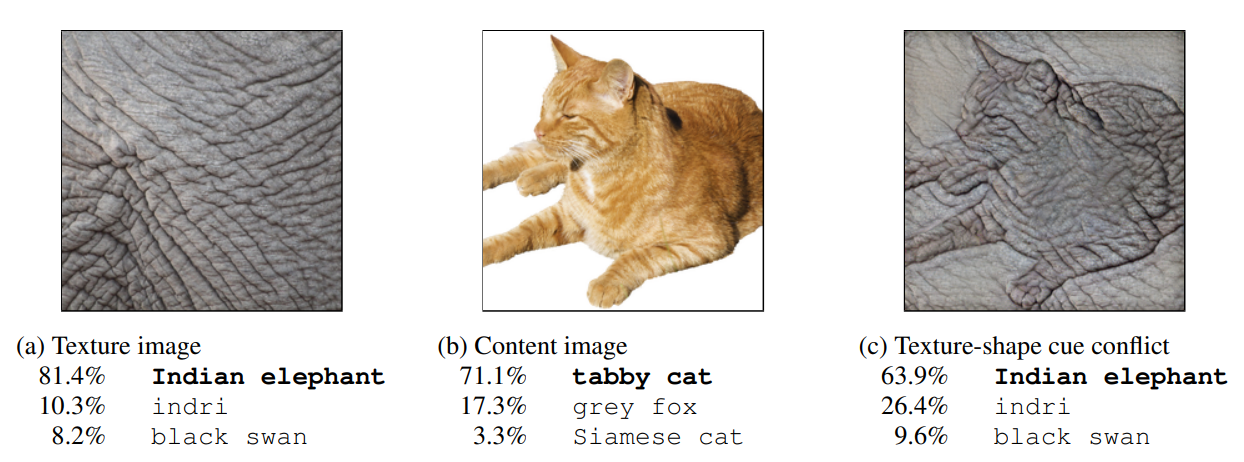
\includegraphics[width=\linewidth]{illustrations/cat_elephant.png}
		\caption{Classifiers trained on ImageNet are biased towards textural features}
		\label{cat_elephant}
	\end{figure}
	
	This behaviour of considering correlations over causation can also be found in state-of-the-art image captioning systems, for instance Microsoft Azure's computer vision API and NeuralTalk2 ~\cite{electric_sheep}, wherein the model seemingly hallucinates that it sees sheep when evaluated on grassy pastures or hills. Once again, it is of course natural to expect that sheep can be found in these contexts, but it is not these contexts that define what it means to be a sheep. Grassy pastures and sheep are not causally related, only correlated, but deep learning pipelines lack the nuance required to understand this fact. 
	\begin{figure}[h]
		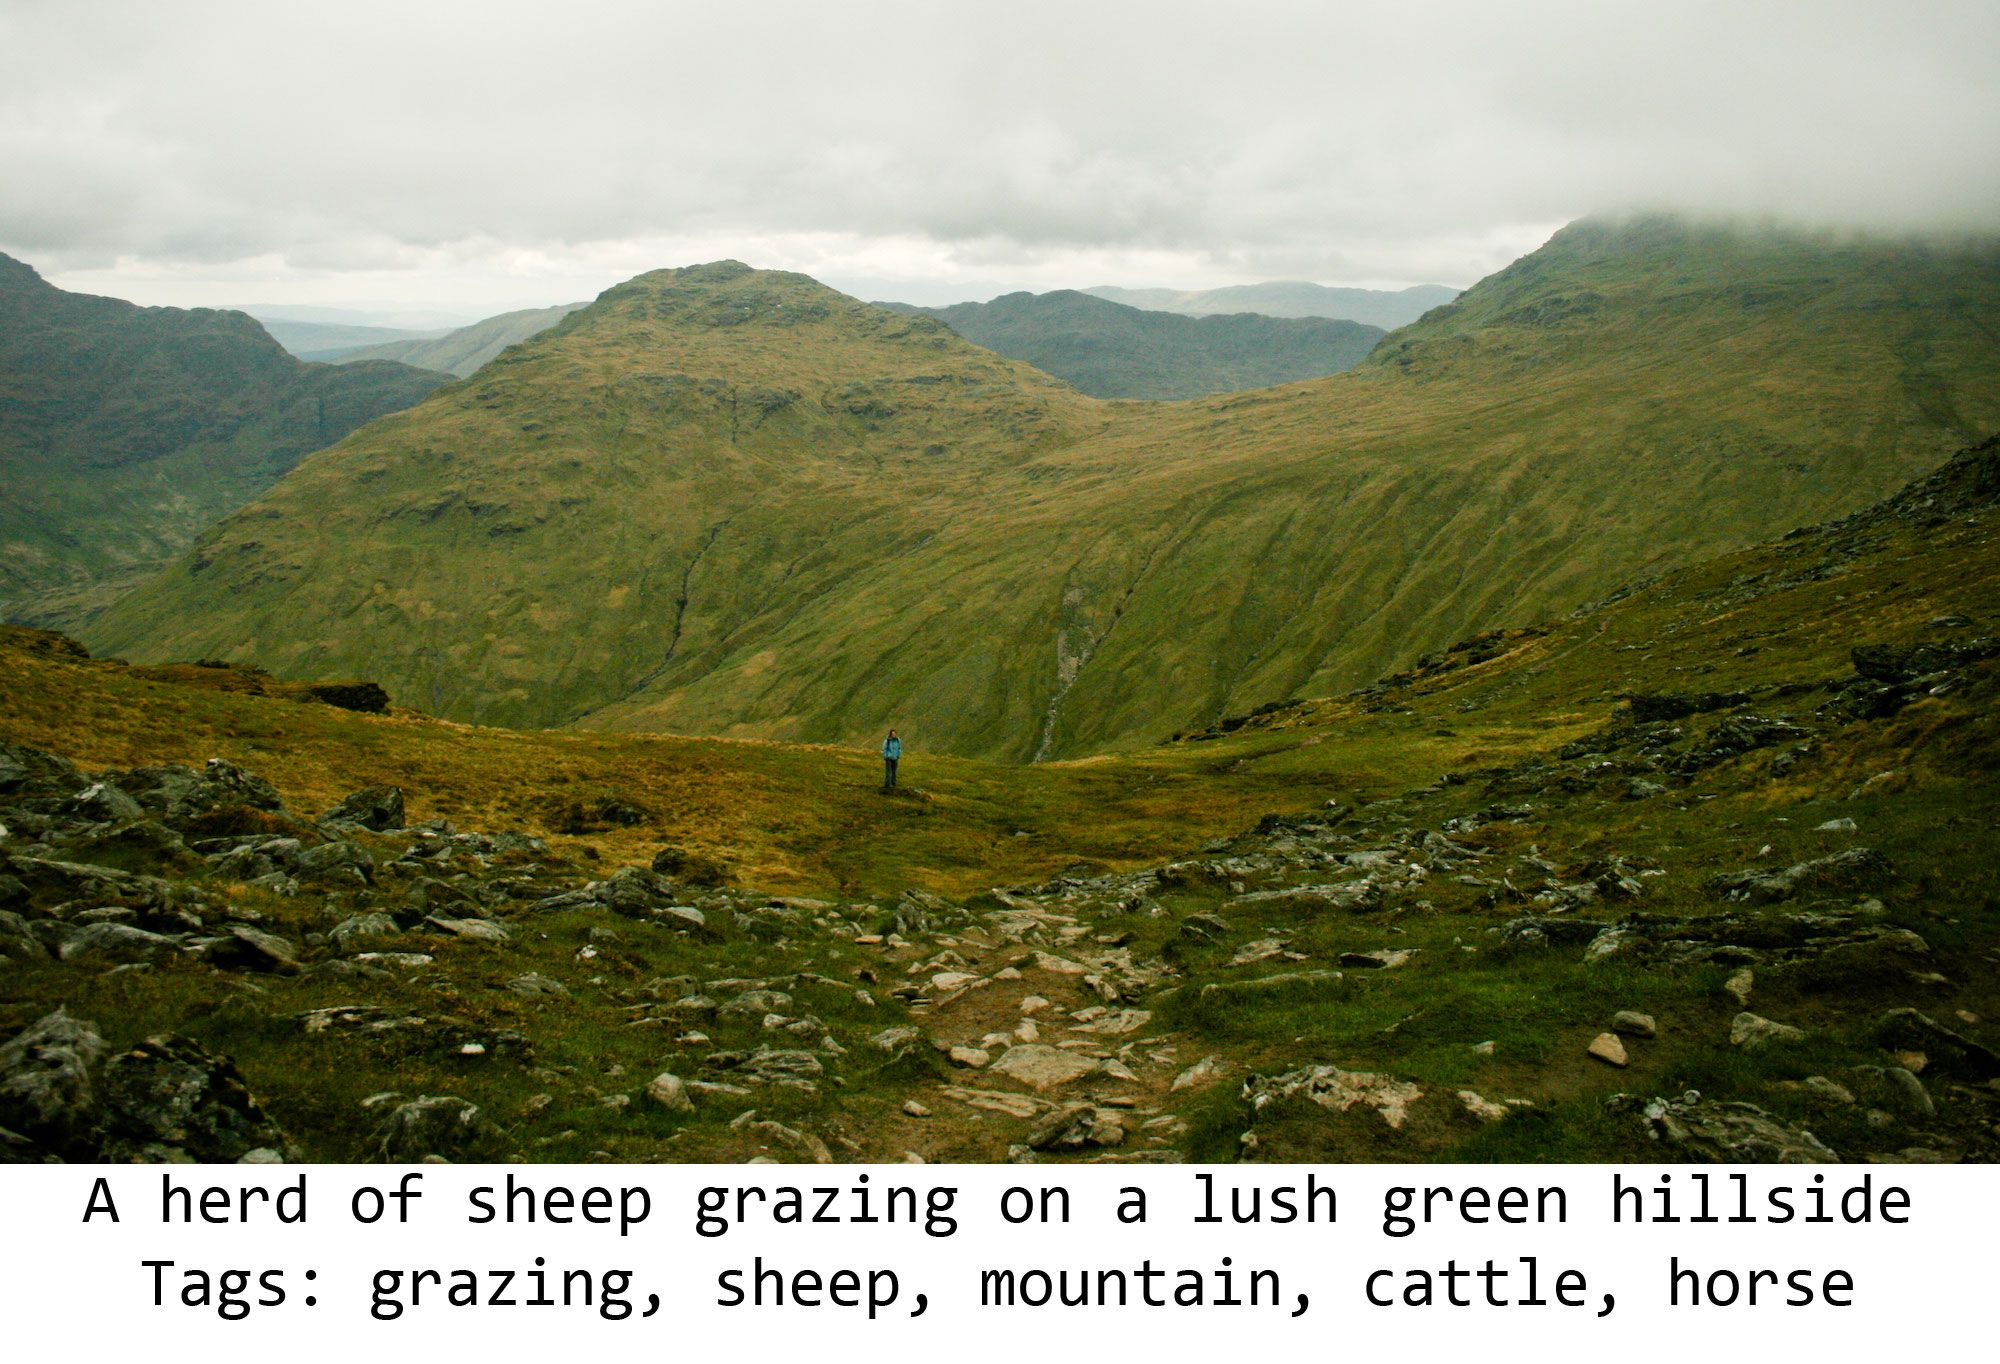
\includegraphics[width=\linewidth]{illustrations/sheep.jpg}
		\caption{Deep captioning models hallucinate sheep when presented with contexts highly correlated with sheep. Adapted from ~\cite{electric_sheep}}
		\label{sheep}
	\end{figure}


	Another characteristic of deep learning that supports this argument is the effectiveness of adversarial attacks ~\cite{adversarial_bugs_features}, which specifically target weaknesses in the inductive biases within DNNs through any number of means in an attempt to induce high rates of incorrect, yet highly confident predictions. Gradient-based adversarial attacks, for instance, use the gradients of the model to break even the most sophisticated and well-trained pipelines merely by adding some carefully crafted, yet visually imperceptible noise to the inputs ~\cite{adversarial_attacks}. Even without access to the gradients, there exists a multitude of so-called black-box attacks that only use output samples to generate similarly effective attacks (cite). Finally, it has been shown that adding minor visual distractions to objects, for example adding bits of tape or graffiti to stop signs, dramatically increases misclassification rates ~\cite{physical_attacks}. 
	
\section{Generalizability Theory}
	Exactly why and how DNNs seem to so persistently fail to generalize is a topic of ongoing research, and the available literature seems to suggest that the problem is multifaceted. This section is an attempt to summarize and distil the findings and analyses performed in the literature so far. It will cover the theoretical basis of generalization and why one might expect DNNs to generalize, discuss the key characteristics of generalization failure, and finally why and how these characteristics arise with respect to the theory.
	
	\subsection{Generalization through Empirical Risk Minimization} 
		Naturally, deep learning would not have experienced as much of a revolution in the last decade or so if there was not some semblance of an expectation that their striking performance was generalizable and performant also outside the idealized settings typically involved in research. The theoretical basis that informs this belief in (most) modern deep learning pipelines is the idea of so-called empirical risk minimization, wherein it is assumed that the dataset upon which the model is trained is a representative sample of the distribution of all possible samples in the relevant domain. In other words, it assumes that the dataset is independently and identically distributed (iid) to the domain distribution. To better understand this assumption, it is beneficial to consider it from first principles: 
		
		At the most fundamental level, the goal of machine learning is to learn a mapping between two spaces of objects \(X\) and \(Y\). This mapping, namely the function \(f: X \rightarrow Y\), maps some input object \(x \in X\), an image for example, to a corresponding and application-relevant output object \(y \in Y\), for instance a segmentation mask or class-wise probabilities. It is worth noting, however, that \(f\) is not as much a function in the mathematical sense as much as it is an abstraction of the relationship that the deep learning system is intended to capture. \(f\) cannot as a consequence typically be modelled explicitly. Instead, machine learning systems aim to find a sufficient approximation of this mapping by leveraging a training set \(\{x_i, y_i\}_{0...n}\). This is referred to as supervised learning, and the resulting approximation found using the training set is denoted by \(h: X \rightarrow \hat{Y}\), and typically referred to as a hypothesis.  
		        
		To find such an approximation, we assume that there exists a joint probability distribution over \(X\) and \(Y\), namely \(P(x,y)\), and that the training data \(\{x_i, y_i\}_{0...n}\) is drawn from this probability distribution such that the resulting sample distribution is independent and identically distributed to \(P(x,y)\). This is the so-called iid assumption. By modelling the mapping as a joint probability distribution, one can model uncertainty in the predictions by expressing the output as a conditional probability \(P(y|x)\). In conjunction with a loss-function \(L(h(x),y)\) which measures the discrepancy between the hypothesis and the ground truth, these assumptions allows us to quantify the expected performance of a given hypothesis:
		\begin{equation}
		    R(h) = \mathbb{E}[L(h(x),y)] = \int L(h(x),y) dP(x,y)
		\end{equation}
		Using this framework, one can then find an iid-optimal hypothesis, often called a predictor, by finding the predictor \(h^*\) among a fixed class of functions (defined by network architecture) \(\mathcal{H}\) that minimizes risk:
		\begin{equation}
		h^* = \argmin_{h \in \mathcal{H}}R(h)
		\end{equation}
		
		Since \(P(x,y\)) is not known, however, one cannot compute \(R(h)\) explicitly. Instead, the expected risk has to be estimated empirically, i.e by finding the arithmetic average of the risk associated with each prediction by the hypothesis over the training set:
		\begin{equation}
		R_{emp}(h) = \frac{1}{n}\sum_{i=1}^{n}L(h(x_i), y_i)
		\end{equation}
		This risk can in turn be minimized with respect to the hypothesis class. This is called empirical risk minimization (ERM):
		\begin{equation}
		\hat{h} = \argmin_{h \in \mathcal{H}}R_{emp}(h)
		\end{equation}
		To reiterate, the central idea with this approach to machine learning is that the training data can be considered a finite iid sampling of the underlying distribution. As such, by the central limit theorem, the hold-out performance of the computed hypothesis will approach iid-optimal performance given a sufficient amount of training data and some sufficiently capable training procedure. This should in theory allow deep learning systems to be able to generalize, since the empirical risk in theory can approximate the true risk arbitrarily well given sufficient training data.

		As described in section \ref{case_studies}, ERM nonetheless readily fails to generate generalizable predictors with respect to out-of-distribution data. There are multiple dimensions to this phenomenon, as there are several means by which a model can fail to generalize. To better understand these failure modes, it helps to consider the assumptions that are made in the formulation of ERM, namely that:
		\begin{enumerate}
			\item \(f\) exists in \(\mathcal{H}\) \label{underfit}
			\item The optimal predictor can be found solely through minimizing \(R_{emp}(h)\)\label{overfit}
			\item \(\{x_i, y_i\}\) is an IID sampling of \(P(x,y)\) \label{structural_misalignment}
			\item \(\hat{h}^*\) is unique in \(\mathcal{H}\)\label{underspecification}
		\end{enumerate}
		As the following sections will show, violations of any one of these assumptions can and typically will result in generalization failure. 

	\subsection{Realizability and Underfitting}
		Violations of assumption \ref{underfit} corresponds to a well known and fairly well understood form of generalization failure, namely underfitting. One can however argue that underfitting can be all but discounted as plausible explanation for the pervasiveness of generalization failure observed in modern deep learning pipelines. Underfitting occurs when the model simply lacks the complexity required to encapsulate the patterns necessary to form generalizable interpretations of the data. To give a simple example - consider the problem of trying to fit a linear model to the following dataset: 
		\begin{figure}[h]
			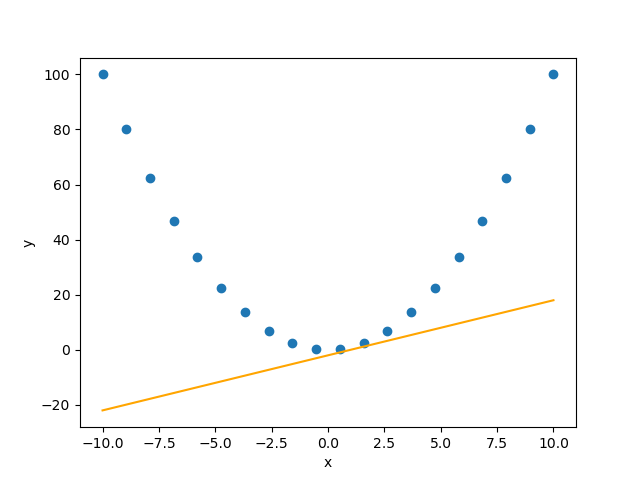
\includegraphics[width=\linewidth]{illustrations/regression_example.png}
			\caption{A linear model cannot fit polynomial data}
			\label{underfit example}
		\end{figure}
		Obviously, no amount of optimization of the parameters in the linear model can ever result in a sufficient description of the underlying data and the function it follows, namely \(y=x^2\). 
		
		This, however, does not necessarily mean that an underfitted model cannot perform well; the above function is after all locally linear, and if it is only evaluated on a limited region, a linear model may perform just fine. One can as such argue that DNNs in turn may be underfitting, and that generalization failure analogously corresponds to evaluating on data outside of this locally linear region. This, however, is unlikely to be the case, as evidenced by recent results in the study of model complexity.
		
		Modern DNNs, as it turns out, have practically infinite so-called effective capacity - i.e, they can model more or less arbitrarily complex data. It can for instance be shown that even a 2-layer feedforward neural network is capable of fitting noise to random labels with 100\% accuracy ~\cite{randomlabels}. Consequently, it is fairly reasonable to expect that the hypothesis space of the highly complex models used today contains a generalizable predictor and thus that assumption \ref{underfit} holds. In the literature, this is often referred to as the realizability assumption ~\cite{machine_learning_theory}. 
		
	\subsection{Overfitting, Inductive biases and training}
	The high effective capacity of DNNs does, however, result in a number of side-effects that actually hamper generalization. Though this capacity does suggest that most learning problems are realizable, the problem of finding a generalizable predictor from the hypothesis space is nevertheless not at all trivial. ERM presupposes assumption \ref{overfit} - i.e that there exists some way to precisely find the risk-minimizing predictor \(\hat{h} = \argmin_{h \in \mathcal{H}}R_{emp}(h)\), and as such that there is some ideal optimization procedure that can be leveraged to this end. This, of course, is not the case. Instead, a search of the hypothesis-space is performed using gradient-descent. On its own, this search is not necessarily guaranteed - or for that matter even likely - to find an IID-optimal predictor. This is due to the inherent nature of the search space - DNNs have parameter counts numbering in the millions or more, and try to determine optimal parameter configurations from comparatively miniscule datasets.
		
	Without certain precautions, this may result in the pipeline returning predictors that in effect simply memorize the training data, without learning anything useful about the domain itself. This is referred to as overfitting. 

	Memorizing all the training data is, however, risk-minimizing. To illustrate, consider a predictor which simply memorizes the segmentation masks for the polyps in a given dataset, and simply returns the corresponding mask when given an image it has trained on, and returns a zero-mask otherwise. This, as explained earlier in this section, is entirely within the capabilities of DNNs due to their high effective capacity. When evaluating this predictor on the dataset upon which is was trained, the empirical risk will naturally be zero, since it will correctly return the right segmentation for a given image despite not having learned anything useful about polyps whatsoever, or for that matter anything useful about images.

	Thus, certain constraints have to be imposed on the search space to avoid overfitting. These constraints have to be defined a-priori, and are often referred to as the inductive biases of the pipeline. 

	This is often achieved through the use of regularization techniques. Dropout, for instance, biases the model towards learning representations that distribute well across the network and can work independently of one another. Weight decay biases the model toward low-magnitude parameters, and thus simpler representations. Data augmentation biases the model towards learning features that hold across augmented samples. Batching biases the model towards features that work well within the batch, and so on.

	Besides regularization, certain inductive biases can also be imposed through modifying the training routines themselves, by for instance pretraining, contrastive representation learning, multi-task learning, pre- and post-processing, early stopping, etc. 

	Determining the effectiveness of these techniques and tuning the hyperparameters that inevitably arise naturally requires a specific evaluation procedure. To this end, most deep learning pipelines leverage hold-out sets, wherein the data is partitioned into three folds - the training set, used to compute gradients and train the model, the validation set, used to tune hyperparameters, and a test-set, used to evaluate the IID generalizability of the resulting predictor. More sophisticated methods, such as cross-validation, are also often used. 

	Fundamentally, each of these techniques increase generalization by limiting the search space, in effect redefining \(\mathcal{H}\). The more inductive biases are imposed onto the model, the smaller \(\mathcal{H}\) in effect will be. 

	Modern Deep learning pipelines regularly employ several of these techniques, often in conjunction with one another, and consequently easily avoid overfitting and achieve good results in IID settings. Nevertheless, they fail to generalize to OOD data. That is not to say that regularization and other ways of imposing inductive biases on the model does not aid in generalization, only that overfitting does not explain the pervasiveness of generalization failure that can be seen today. 

	\subsection{Structural Misalignment and dataset bias}
	Recent research on generalization failure often attributes it to a structural misalignment between the predictor as generated by ERM and the causal structure which it ideally should encode ~\cite{adversarial_bugs_features,shortcut_learning,IRM, causality}. Generally, this misalignment occurs as a result of the predictor learning spurious or otherwise causally unrepresentative features that nonetheless perform well within the training distribution. This if of course made evident as soon as the predictor is exposed to any form of distributional shift, at which point it will (typically) fail to generalize. These distributional shifts can range in magnitude, from changes in imaging modalities, common corruptions such as noise or blurs ~\cite{benchmarking_robustness} or spatial transforms ~\cite{spatial_robustness} to practically imperceptible perturbations, typically exemplified by adversarial attacks ~\cite{adversarial_attacks}. ERM does not and cannot guarantee invariance to distributional shifts, as it assumes that the training data is IID to \(P(x,y)\). This is not, however, necessarily as much of a flaw with ERM inasmuch as it is a flaw in the reasoning behind our expectations. 
		
	To illustrate, consider the rather pertinent example of training a model exclusively on either white-light or narrowband endoscopy. Assume that there are two datasets, each containing samples depicting identical scenes, with the only difference being that dataset A employs white-light endoscopy, whereas dataset B employs narrowband endoscopy. Ideally, a model trained on either dataset should generate predictors that can generalize to the other, and though one may be optimistic and hope this is the case, this is in no way guaranteed. The causal structure behind the decisions - i.e what exactly makes a polyp a polyp - is never considered at any point in the training process. Instead, the models will simply try to leverage whatever predictive patterns can be found the training data. The model trained on narrowband images may for instance principally consider the textural characteristics of the polyps, which narrowband endoscopy enhances. Conversely, the model trained on white-light images, lacking access to these textural characteristics, may instead consider more colour- or shape-based features. Naturally, if this narrow-band-texture-biased model is deployed in white-light endoscopy, it is not likely to succeed since its principal discriminative features no longer are particularly useful. Similarly, the colour-biased model would fail when deployed in narrowband endoscopy since the colours it once used to distinguish polyps are no longer predictive in narrowband images.  

	\begin{figure}[h]
		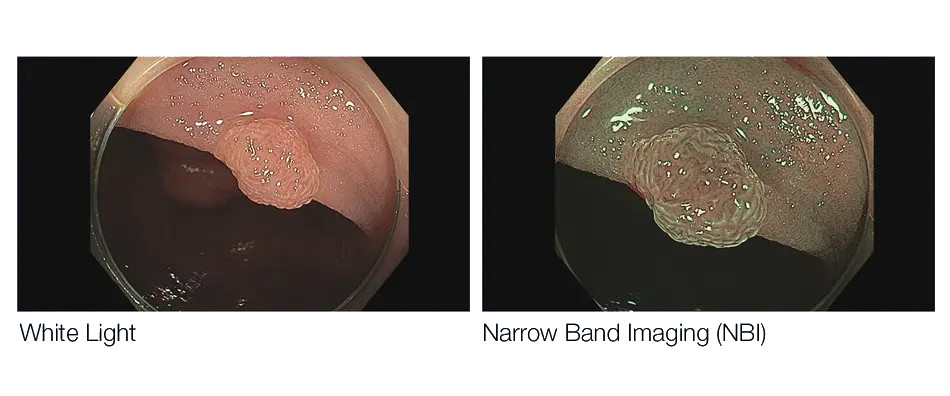
\includegraphics[width=\linewidth]{illustrations/narrow_band.jpg}
		\caption{Narrowband imaging and white-light endoscopy constitutes a distributional shift. Adapted from ~\cite{nbi_img}}
		\label{imaging_modalities}
	\end{figure}

	Though the features each model learns are not particularly representative of the broader context of what makes a polyp a polyp, they make sense when considered from the perspective of either of the two modalities. When considering only narrow-band imaging, it makes some sense to heavily weigh the texture of the polyps. When considering only white-light imaging, it makes some sense to heavily weight the shape and colour of the polyps. Though humans are capable of appreciating broader context and subconsciously know that certain features are ancilliary rather than causal (and perhaps more importantly: know the strengths and weaknesses of each modality), DNNs lack the inductive biases needed to take this into account. Once again, DNNs merely leverage the first and best predictive patterns found during the training process, and cannot be expected to optimize for specific invariances on their own, irrespective of how self-evident these invariances may be for humans. This predilection towards dataset-specific features is aptly referred to as dataset bias. 
	
	\subsubsection{Shortcut Learning}
	In the aforementioned example, though the features each predictor learns is not robust to dataset shift, they nevertheless have causal explanations. The causal structure that they correspond to is of course not dataset-agnostic, and as a result flawed in their own way, but the patterns the respective models leverage to interpret the data are not particularly irrational. As it turns out, however, DNNs are unlikely to learn such causally viable features in the first place. In other words, the predictors would not necessarily learn to consider texture in narrow-band images - it could learn any arbitrary pattern so long as it is predictive. Moreover, if such interpretable distributional shifts were the principal cause of generalization failure, generalizability could be practically guaranteed by explicitly modelling the effects such shifts induce and taking this into account in the pipeline. In the aforementioned example, one could for instance train some model to map from one lighting environment to the other. Though this would imbue the model with an inherent invariance to the choice of lighting, it is nonetheless not given that the resulting model will be perfectly generalizable.

	Consequently, though these detectable forms of distributional shifts also hold some importance when designing generalizable models, a more pervasive and substantially more significant issue is the fact that many of the distributional shifts encountered in clinical settings are not necessarily considered significant or for that matter at all perceptible to a human observer. A human would for instance not be significantly affected by slightly noisy, blurry, rotated, or compressed images, nor would they in all likelihood notice these perturbations. DNNs, on the other hand, have been shown to be highly sensitive to these and several other forms of minor perturbations ~\cite{noise_robustness, corruption_robustness,adversarial_training,benchmarking_robustness}. Moreover, a human would likely not pick up on subtle phenotypic cues that may exist in the colon during endoscopy, whereas a DNN may leverage some of these cues to inform their decisions, and hence exhibit varying performance across different demographics. 

	It is important to note, however, that despite how these two forms of distributional shift may at surface level appear as completely separate classes of problems, they can both be traced to the same phenomena - namely that DNNs do not leverage any form of causal logic to inform their decisions and, as mentioned previously, simply exploit any sufficiently predictive pattern they may observe in the data. This phenomenon has been shown to be pervasive across all manner of domains, from natural language processing and computer vision to reinforcement learning and algorithmic decision-making. This is referred to as shortcut learning ~\cite{shortcut_learning} or the Clever Hans effect ~\cite{cleverhans}. 

	Shortcut learning and the brittle features it corresponds to have also been identified as one of the key properties that explains the effectiveness and pervasiveness of adversarial attacks ~\cite{adversarial_bugs_features}. Naturally, a generalizable predictor should be robust to such minor perturbations, as the model should not in the first place be learning features that get perturbed to any significant degree by adding such high-frequency, low-amplitude noise. Adversarial attacks simply leverage the high degrees of sensitivity inherent to shortcut features, and construct perturbations according the direction in the search space that corresponds to the principal component of this sensitivity ~\cite{sensitivity}. 

	\begin{figure}[h]
		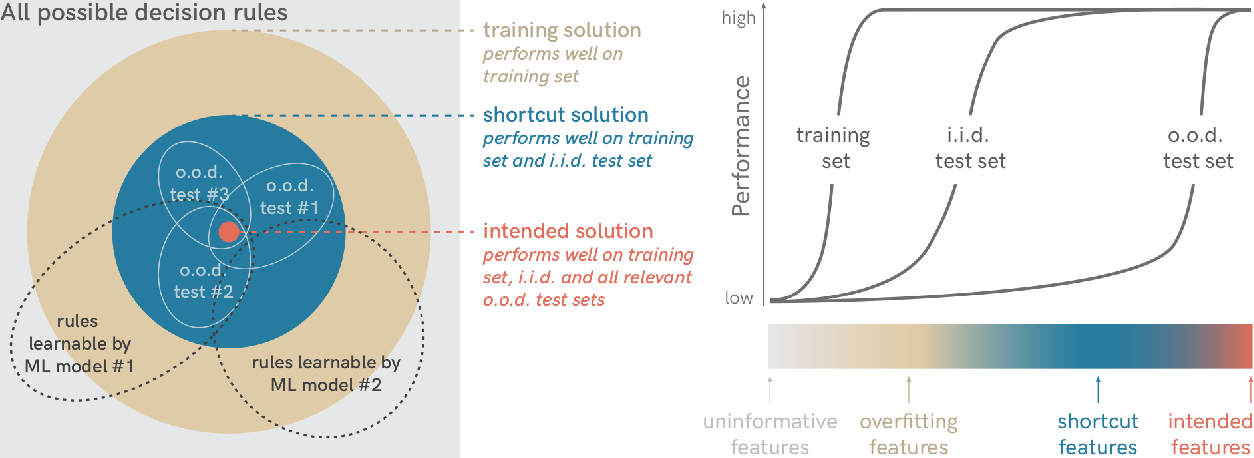
\includegraphics[width=\linewidth]{illustrations/features.png}
		\caption{Taxonomy of feature types. Adapted from ~\cite{shortcut_learning}}
		\label{feature_types}
	\end{figure}


	\subsection{Underspecification}
	Closely related to shortcut learning is underspecification ~\cite{damour2020underspecification}. A machine learning pipeline can be considered underspecified when it can return any number of risk-equivalent predictors when evaluated on an iid holdout set, dependent only on the random variables used within the training procedure - i.e dropout, seed initialization, and so on. Even with identical hyperparameters, a given training procedure can return any number of predictors each having learned different patterns. One predictor may have learned one shortcut, another may have learned a different shortcut, and one may have fully learned the actual causal relationships it is intended to. With ERM, and in particular with iid-oriented evaluation procedures, these are all erroneously considered equivalent. 

	Note that this does not however presuppose anything about the relative occurrence rates of generalizable and non-generalizable predictors. It may not necessarily even be the case that the pipeline can return a generalizable predictor at all. Only that there exists a multitude of risk-equivalent predictors in the search space the optimizer typically explores. Nor does it presuppose anything about the distribution of predictors, only that there is indeed a distribution. 

	This is evidenced by the fact that generalizability can vary greatly depending on the choice of random seed used during training. In the foundational paper on underspecification in deep learning, for instance, it was highlighted that certain classification pipelines can produce predictors that vary in ood accuracy by up to 10\% ~\cite{damour2020underspecification}. This is a function of the robustness of the learned features and how likely the pipeline is to return the corresponding predictors. 
	\subsection{A probabilisitic perspective of generalization}
	As established, modern deep learning pipelines are not capable of reliably returning generalizable predictors. However, they are not necessarily precluded from it. One can to some extent model this probabilistically by considering the distribution of parameters given the training data, \(p(w | \mathcal{D})\). Though it is impossible to know which part of this distribution corresponds to generalizable predictors, it has been shown that marginalizing over this distribution - in other words, bayesian learning - increases generalizability ~\cite{bayesian_generalization,endoensemble,divergentnets,ensemble_machinereading}. 

	~\cite{bayesian_generalization} provides a probabilistic perspective of this phenomenon. They consider generalizability as a two-dimensional quantity, consisting of the support and inductive biases of a model. The inductive biases are as mentioned the constraints by which the model learns, ranging from model-construction - e.g positional invariance in CNNs - to regularization - e.g dropout, data augmentation, etc - and specific training routines - i.e multitask learning, contrastive representation learning, etc. The support, on the other hand, describes the ability of the model to encode certain decision rules. Ideally, and as is the case in deep learning, support should be maximized, as the model should be able to learn as complicated decision rules as may be required by a given problem. Similarly, and perhaps intuitively, the amount of inductive biases imposed on the model a-priori should also be maximized, as it reduces the probability of learning spurious correlations. 

\section{Related work on generalizable deep learning}
%TODO add figures from papers here
To summarize, generalization failure occurs due to the weaknesses inherent to ERM. The features that ERM learn to incorporate are often spurious, and the predictors that leverage them are often returned practically arbitrarily from the pipeline. The approaches that have exhibited the highest degrees of success towards increasing generalization as a consequence tend to address these issues in some way or another. 

One of the most well-studied approaches to increasing generalizability is the use of data augmentation. Data augmentation is typically implemented in deep learning pipelines in order to prevent overfitting, often in conjunction with other regularization methods. Naturally, overfitting also constitutes generalizability failure in its own right, but augmentation has also been shown to have positive effects for out-of-distribution generalization. It has for instance been shown that carefully designing augmentation procedures increases the generalizability of polyp segmentation models ~\cite{polyp_augmentation} and prostate segmentation ~\cite{augmentation_prostate}. There has also been a large body of work dedicated to leveraging recent advances in generative models such as generative adversarial networks (GANs) and variational autoencoders (VaEs) to serve as synthetic data augmentation. These types of approaches have also been shown to increase generalizability in CT segmentation ~\cite{cyclegan} and x-ray based covid detection ~\cite{covid}. Data augmentation facilitates generalization by implicitly imbuing the pipeline with more credible inductive biases, as the empirical risk will be best minimized by leveraging features that are conducive to minimizing risk across both synthetic or otherwise augmented data and unaugmented data. Naturally, the choice of augmentations that are used is an inductive bias in and of itself; by employing random rotations, rotational invariance is presupposed. By employing random cropping, image-space object size invariance is presupposed. By employing additive noise, invariance to additive noise is presupposed, and so on. From an ERM perspective, this can also be thought of as improving the empirical risk estimate; given enough data, all of these invariances may be learned automatically. With a finite and often fairly limited dataset, this may not necessarily be the case simply due to the large number of confounding variables involved. 

Another type of approach involves biasing the pipeline towards learning more structured and causally viable latent representations. This is also somewhat well understood when considered through the lens of regularization: drop-out and weight-decay are often employed in order to reduce overfitting under the assumption that a generalizable predictor should not base its decisions on only a few of the available neurons and that separate neurons should instead encode independent representations of the input. Though there is limited research on the effects of dropout on ood generalization, constraining the latent representations in DNNs has been shown to be effective method to increase generalizability. For polyp-segmentation it has for instance been shown that adding context-based attention layers to multiple blocks in a given network results in state-of-the-art IoU scores for out-of-distribution evaluation on certain datasets ~\cite{uacanet}. Other attention-based approaches have also shown promise in this regard ~\cite{attention_generalizability, reverse_attention}. This permits the model to learn and generate attention maps for its latent representations, thus in theory biasing the model towards learning more a more structured interpretation of the data. 

Multi-task and/or multistage learning has also been leveraged to this end. By jointly optimizing for multiple tasks/subtasks, the model can be biased towards learning features that describe the input data well independent of their performance on any one of the relevant tasks. For polyp-segmentation, for instance, it has been shown that adding image reconstruction as an auxiliary task ~\cite{ddanet} or decoupling the segmentation task into a coarse segmentation and refinement stage ~\cite{doubleencdec} increases generalizability. 

More closely supervised methods, wherein certain inductive biases have been explicitly introduced to the pipeline, have also been shown to have some promise. One paper for instance reported an increased robustness to image perturbations after adding a custom filter bank designed to emulate the primary visual cortex of primates to the front of the CNN ~\cite{visual_cortex}. Another reported that models trained on imagenet exhibited significantly higher robustness when explicitly biased towards shape-based features ~\cite{texturebias}. 
	
These approaches all provide workarounds to flaws with ERM, typically to limited practical effect. Consequently, a growing body of work has instead been investigating the idea of foregoing ERM altogether in favour of developing alternative training paradigms. In so-called Invariant Risk Minimization~\cite{IRM}, for instance, the model trains to ignore spurious correlations by optimizing for predictors that exhibit stable performance across multiple training environments. A similar approach, namely model-based robust deep learning ~\cite{modelbased}, employs a similar idea in conjunction with distributional modelling. The model is trained such that it is robust to perturbations as generated by a so-called model of natural variation. If this model for instance describes the function mapping one training environment to another, this will then optimize for predictors that are invariant to the distributional shift this function corresponds to. 

Finally, Bayesian learning has also been shown to improve generalization. In particular, ensemble-based networks - which mathematically can be considered an approximation of Bayesian marginalization ~\cite{bayesian_case,bayesian_generalization} - have demonstrated high degrees of generalizability for polyp-segmentation ~\cite{divergentnets,endoensemble}. Since deep learning pipelines are typically underspecified, one can consider an ensemble of predictors to be a sampling of the distribution over parameters given training data. These predictors are of course unlikely to have learned identical representations, and consequently whatever spurious correlations inferred by one predictor may be countered by the features employed in another. Consequently, features that are stable across predictors and consequently more likely to generalize are weighed to a greater extent, in turn mitigating the effects of underspecification. Structural misalignment may nevertheless impact ensembles, and as such the effective returns are limited. 


    \chapter{Methods}\label{methods}
Summarizing the key points made in \Cref{background}, current deep learning pipelines are not equipped with evaluation methods suitable for out-of-distribution generalization, are largely incapable of reliably learning causally robust features, and are underspecified by the datasets they are trained on. Addressing generalization failure requires mitigating some of these problems. The literature, in broad strokes, tackles this by improving the models' inductive biases, e.g., through attention-based mechanisms~\cite{attention_generalizability, reverse_attention}, ensembles~\cite{divergentnets, endoensemble}, or their support like data augmentation techniques~\cite{polyp_augmentation, cyclegan}. 

This thesis attempts to combine the central ideas behind these methods into one unified deep learning pipeline, intended primarily to maximize generalizability. The contributions can be summarized as following:

\begin{itemize}
    \item A modified DeepLabV3-based model with dual decoders, intended to constrain the space of latent representations such that underspecification is mitigated.
    \item A new view of generalization as consistency with respect to a hidden perturbation model, as well as a corresponding training procedure, metric and loss-function.
    \item An augmentation strategy informed by this alternative view, including both conventional augmentation functions and a \gls{gan}-inpainter decoder.
    \item A family of ensemble models consisting of predictors trained according to the above methods.
\end{itemize}

\section{DD-DeepLabV3+}
As described in \Cref{background}, generalization failure can in part be attributed to the fact that most deep learning models are underspecified by the training data. In other words, the same pipeline can return any number of risk-equivalent predictors that leverage significantly different features. To mitigate this, one may impose constraints on the space of features that a given model can learn, such as through multi-task learning~\cite{ddanet}, attention-mechanisms~\cite{attention_generalizability, reverse_attention} and preprocessing~\cite{visual_cortex}. 

As testing the relative effectiveness of all of these different approaches is beyond the scope of this thesis, a simple model is instead introduced, namely a dual-decoder DeepLabV3+. As its name suggests, this model is functionally equivalent to a standard DeepLabV3+~\cite{deeplab}, but is endowed with an additional decoder, which performs image reconstruction. In theory, this should constrain the model such that it learns features that are conducive to both segmentation and reconstruction simultaneously. This constraint should mitigate underspecification and force the model to learn more generalizable features, as the feature space that is conducive to both reconstruction and segmentation naturally should be smaller than the feature space conducive to segmentation only. This does, however, presuppose that features conducive to image reconstruction also are conducive to segmentation, which may not be the case. A diagram of the model is shown in~\Cref{fig:dddeeplabv3}.
\begin{figure}[htb]
    \centering
    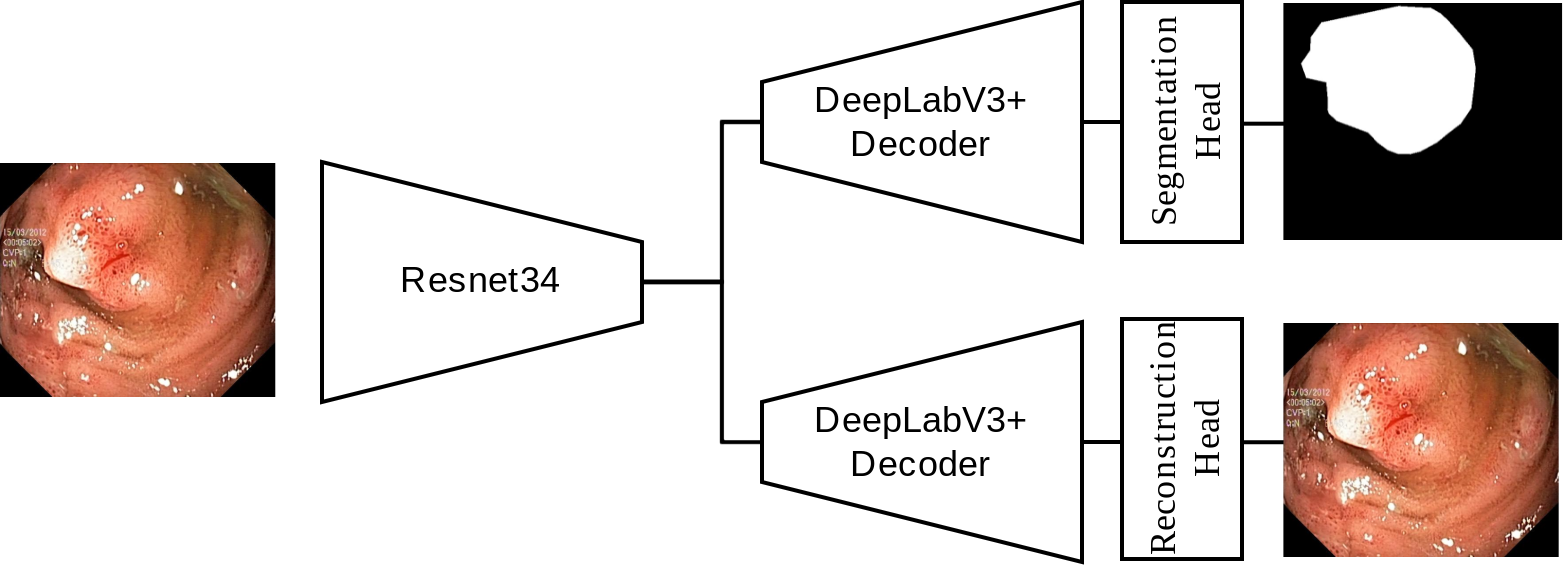
\includegraphics[width=\linewidth]{illustrations/InductiveNet.drawio.png}
    \caption[Dual Decoder DeepLabV3]{Diagram showing the Dual-decoder DeepLabV3+ model. This model uses a ResNet34 encoder to generate a feature map, which is then leveraged by two decoders concurrently. One decoder performs polyp segmentation, and the other performs image reconstruction. Functionally, the decoders are identical, and differ only in that the segmentation decoder requires sigmoid activation to map the output logits to a probability map one channel wide, whereas the reconstruction outputs the pixel values directly to three channels}
    \label{fig:dddeeplabv3}
\end{figure}

As discussed in \Cref{experiments}, this model also has the advantage of being easily compared to the standard DeepLabV3+; the part of the dual-decoder network responsible for segmentation is after all functionally identical to the single-decoder network. This facilitates better analysis of the impact of the additional decoder and its effect on the learned features, as the performance of the respective models can be compared directly. 

\section{Consistency Training}
This section will introduce Consistency Training, a training procedure wherein the objective is to optimize for invariance to a set of various image transformations by quantifying the degree to which the model outputs inconsistent predictions when its input is subjected to some transformations. This is achieved by training with two images: one which is augmented, and on which is not. The given model then performs inference on these two images, resulting in two segmentation masks. The difference between these two predictions is then computed, and compared to the difference (if any) between the augmented and unaugmented segmentation labels. This is then incorporated into the loss-function such that the discrepancy between the expected prediction change and actual prediction change is minimized. This is illustrated in~\Cref{fig:consistency_training}. The next sections will cover the theoretical basis of this training procedure as well as the implementation of its constituent components.  

\begin{figure}[htb]
    \centering
    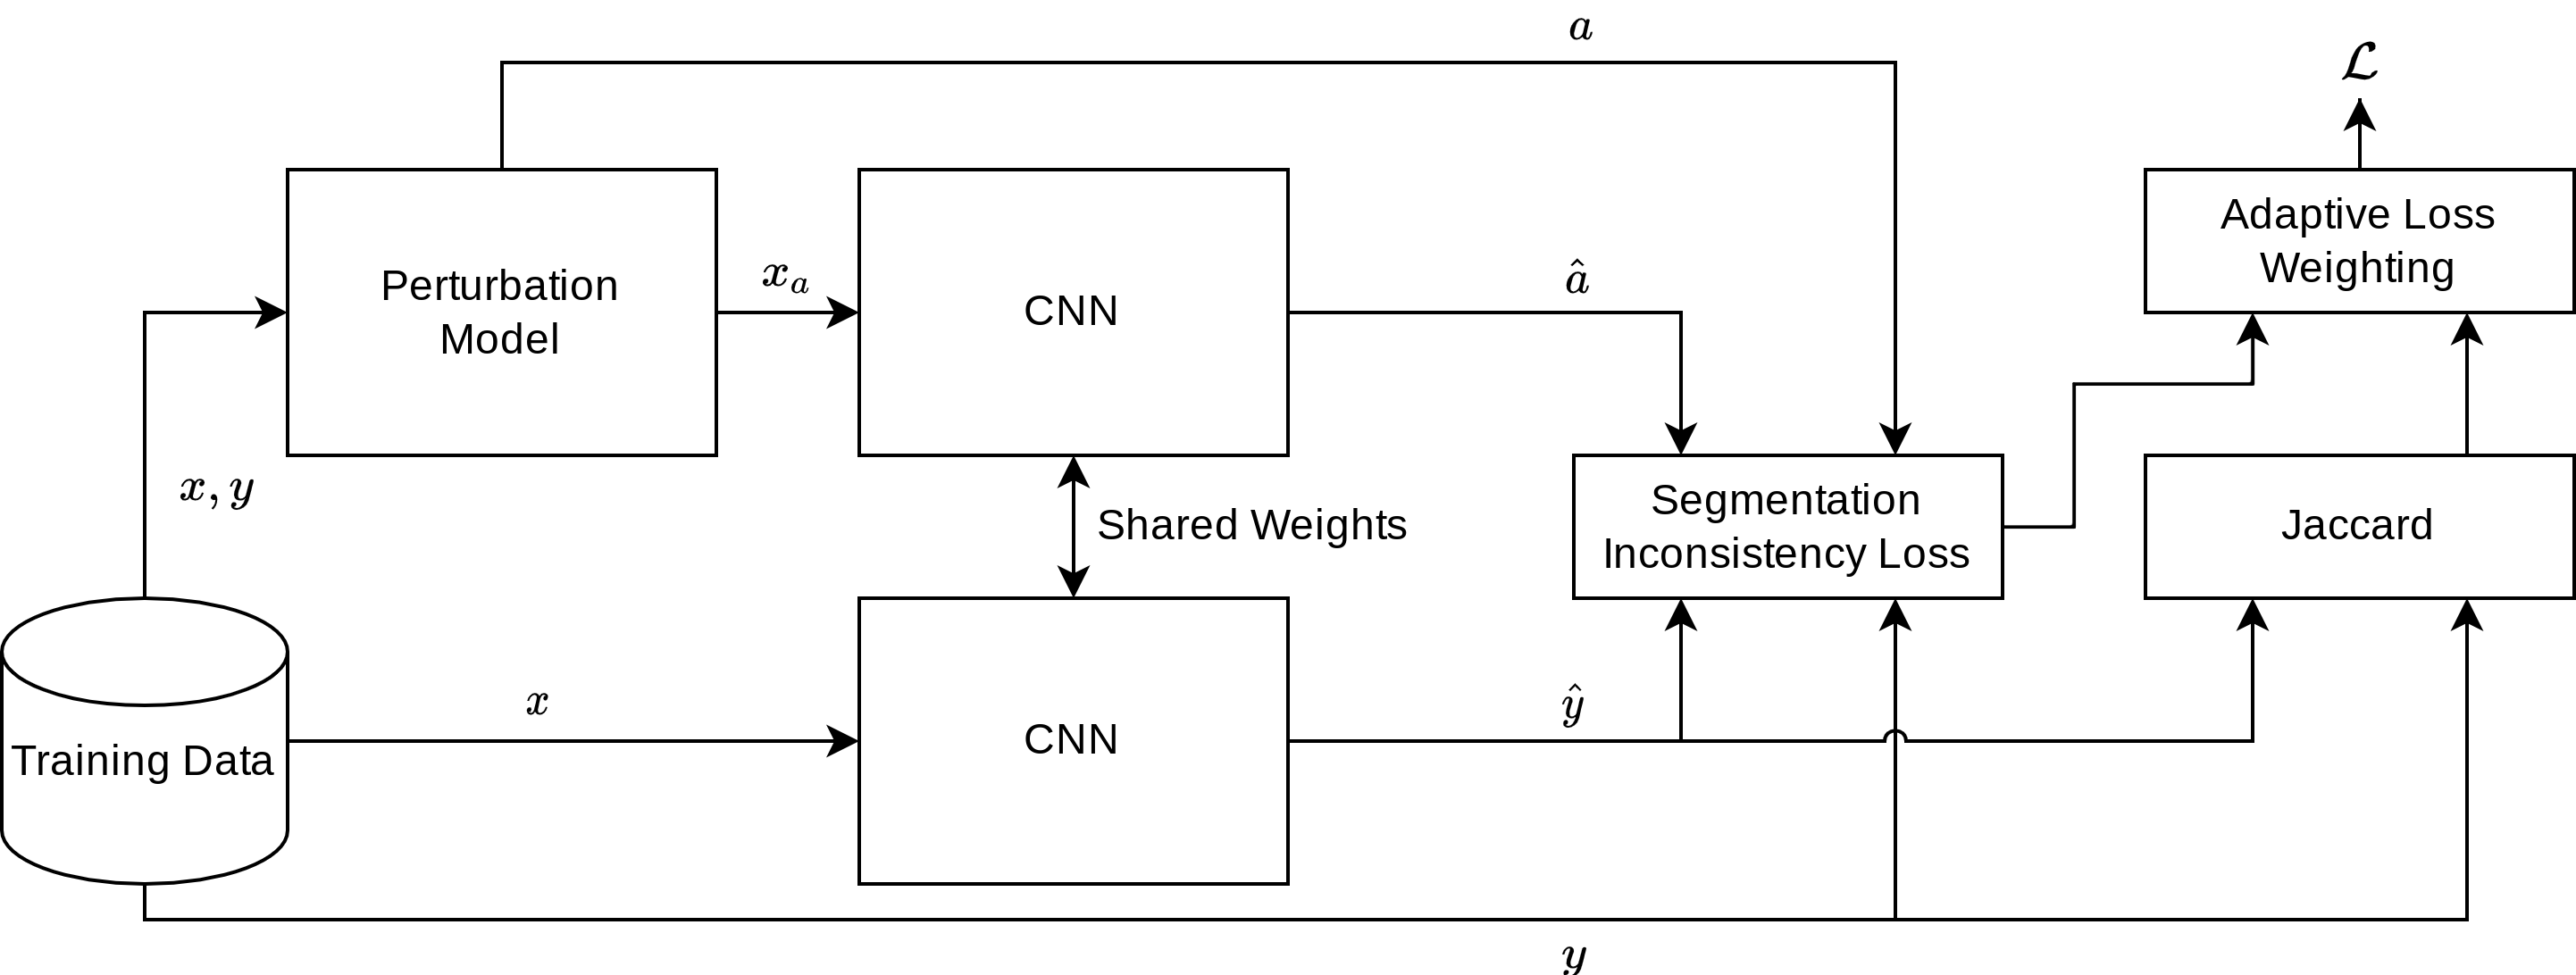
\includegraphics[width=\linewidth]{illustrations/consistency_training.png}
    \caption{Consistency Training}
    \label{fig:consistency_training}
\end{figure}


\subsection{Consistency as a Surrogate for Generalization}\label{consistency_conceptual}
As discussed in \Cref{background}, distinguishing between generalizable and non-generalizable predictors, and in turn optimizing for generalizability directly, is not feasible when evaluating only in iid-settings. This is because there is no way of knowing whether the features learned through \gls{erm} are causally related to the problem, or if they are simply predictive due to some other correlation that is strong exclusively within the bounds of the distribution given by the training data. A generalizable evaluation procedure therefore requires some way of determining whether the predictor is leveraging non-causal or causal features. 

Determining what features are causally related to the problem is, however, somewhat of an intractable problem. First and foremost, the patterns that neural networks learn and the logic that underpin them are often difficult to identify, and even more difficult to interpret on an intuitive level. Secondly, assuming there was some way of understanding these factors perfectly, establishing causality with any certainty necessitates a higher level of understanding of the problem than is reasonable to expect. 

Though establishing what \textbf{is causal} is difficult or even impossible, establishing what \textbf{is not causal} is not all that complicated. To give a concrete example, consider the problem of classifying images of cows in grassy pastures and camels in deserts. A deep learning model may just as easily learn to associate the "cow" class with grass and the "camel" class with deserts as learning what actually constitutes the respective animals. Thus, it may predict that a camel standing in a pasture or a savanna is a cow, or equivalently predict that a cow standing in a desert or on a beach is a camel. This is illustrated in~\Cref{fig:cows_and_camels}.

\begin{figure}[htb]
    \centering
    \includegraphics[width=\linewidth]{illustrations/cows_and_camels.png}
    \caption[Cows and Camels Example]{A model trained on Cows in pastures and camels in Deserts may learn to associate the cow class with grass and the camel class with sand, and thus fail to generalize even if performance on an \gls{iid} test-set is exceptional}
    \label{fig:cows_and_camels}
\end{figure}

Associating the cow class with grass and the camel class with sand is obviously non-causal, however, since this pattern would not hold if the model for instance is asked to detect cows on Mars or camels on the Moon. To mitigate this, ones first instinct may be to simply collect data of these cows and camels in a wide assortment of differing backgrounds - i.e, increasing the models' support - but such careful curation of datasets is not typically feasible, and is at any rate not guaranteed to solve the problem, as another shortcut may easily be found. In the context of polyp segmentation, is for instance not feasible to collect a dataset that is fully representative of all the differing demographics, imaging equipment, endoscopy operator faults, and so on that one may expect in deployment.  There is simply too much variation to be fully accounted for. Instead, one has to leverage the data that is actually available and try to squeeze as much utility as possible from it, either by imposing some number of a-priori inductive biases or by increasing the models' support through augmentation.

Once again going back to the cows and camels example, one may for instance generate multiple instances of the same cow but with varied backgrounds and punish the model for predicting differently depending on the background. This way, the inductive bias that the predictor should be invariant to backgrounds is imposed, and the model is given more support simply by being exposed to differing data. 

This, of course, applies to more than just modifying backgrounds: the more of these non-causal changes to the input data are accounted for and modeled, the more spurious correlations are excluded from the search, the more likely the model is to learn the patterns that are actually causal. These sorts of non-causal changes to the data will from this point on be referred to as \textit{perturbations}. These perturbations can take practically any form, only under the condition that it should not affect the causal structure of the data. If a model is trained such that invariance to all such perturbations is achieved, it must necessarily be leveraging causal features and thus be generalizable. After all, a given set of features can for all intents and purposes be considered to be causally related to the problem when the predictions generated therefrom hold when subjected to all possible perturbations. 

Thus, though rewarding causal behaviour is intractable, punishing non-causal behaviour is not. All that is required to do so is to be able to apply perturbations that highlight the non-causal reasoning the model employs, quantify the model's sensitivity to these perturbations, then minimize this quantity through optimization. The resulting model will then in theory have learned invariance to whatever causally irrelevant information that the perturbations define. This property of being invariant to perturbations will be referred to as the \textit{consistency} of the model. 

This notion of consistency can in effect be considered a surrogate for generalizability; if a model is consistent to all perturbations, it is invariant to non-causal patterns, and if it is invariant to all non-causal patterns, it necessarily employs causal patterns. Optimizing for consistency can as a result mitigate generalization failure, subject only to the span of the perturbations and how well inconsistent behaviour can be quantified.

This line of reasoning does presuppose that there is some model that can output all possible perturbations one might desire the model to be invariant to. This is of course not the case. As highlighted by the pervasiveness of adversarial attacks and the relative ineffectiveness of adversarial defenses, the perturbations that break DNNs are not necessarily intuitive, and are often difficult to analyze in a manner that is conducive to the task of engineering invariances. Nevertheless, much stands to be gained if the model learns to be invariant even to a fairly limited space of perturbations. Though generalizability is by no means guaranteed in this case, the odds of learning generalizable features are nevertheless improved simply because imposing invariance to a set perturbations limits the types of patterns that a given model can learn. If for instance a white-light endoscopic image is perturbed such that it mimics a narrow-band image, and the model learns to be invariant to this perturbation, predictors that leverage white-light or narrow-band dependent features will no longer be returned from ERM.

This approach, then, requires two components: a perturbation model, and a loss function that can describe inconsistent behaviour subject too these perturbations. One can then in turn optimize for consistency through gradient decent. The implementation of these two components will be covered in the following chapters.
    
\subsection{Implementing a Perturbation Model} \label{perturbations}
So far, it has been assumed that a perturbation model was given beforehand. This is of course not the case, and naturally any such model needs to be designed with respect to the domain in question. Rotational invariance makes sense for endoscopic images, for instance, but not for classification of hand-written numbers. Thus, in order to engineer such a model, it is first necessary to establish what invariances are desired for the given task. In the case of polyp-segmentation, it is clear that it is necessary to account for variability in for instance lighting, image-resolution, polyp-size, polyp-shape, polyp-location, camera-quality, color-shifts, blurs, optical distortions, and affine transformations. Thus, a model is required that can (more or less) parameterize this variability. Broadly speaking, these transformations can be categorized as follows:
\begin{itemize}
    \item Pixel-wise variability, which affect only the image, i.e color-shifts, brightness shifts, contrast-shifts,  blurs etc. Practically, this corresponds to changes in lighting conditions, camera motion, dye applications, etc.
    \item Geometric variability, which affect both the image and the segmentation mask, for instance affine transforms and other spatial distortions. Practically, this corresponds to endoscope orientation, optical distortion in the camera, zooming, etc. 
    \item Distributional variability, which affects both the image and the segmentation mask depending on a learned model of the distribution. Practically, this corresponds to the size, shape and location of the polyps
\end{itemize}
Pixel-wise variability and geometric variability can be modelled fairly trivially through the use of the same transformations typically used in conventional data-augmentation. Distributional variability, however, is somewhat more difficult, and requires a model that can sufficiently represent some characteristic of the distribution. This can for instance be achieved via and cross-dataset style-transfer~\cite{cyclegan, modelbased}, but this of course necessitates multiple datasets. Given only one dataset, a different method must be used. For a classification task, this could for instance be DeepAugment~\cite{deepaugment} or a similar technique. DeepAugment, however, cannot account for the changes in the segmentation mask that should be induced by the augmentations it generates. Consequently, some other generative model wherein the changes in the segmentation mask can be accounted for is required. To this end, a \gls{gan}-inpainter can be used. 

\subsubsection{GAN-based Polyp Inpainting}
As mentioned in \Cref{background}, the use of GANs and other distributional modelling in the context of generalization is typically restricted to image-to-image translation, and typically involves transforming an image drawn from one distribution such that it is \gls{iid} with a second distribution. This, though interesting and no doubt useful assuming several such datasets are available, has limited practical use. It is not necessarily always the case that there exists multiple datasets depicting identical problems, and merely translating between modalities does not as mentioned earlier in the thesis ensure generalizability.

A better approach is to try to model the training set distribution directly, then perturb the data in accordance with this model. For segmentation problems, this can be achieved through training a model to fill some predefined region with pixels that correspond to whatever segmentation target the model is meant to learn, in this case polyps, then perturb a given sample by for instance increasing the size of the polyps or adding extra polyps.

To this end, a simple GAN-inpainter was trained. The Generator \(G(\cdot)\) and Discriminator \(D(\cdot)\) were both implemented with the DeepLabV3+ architecture, and trained using the following loss formulation, where \(L_d\) and \(L_g\) corresponds to the discriminator and generator loss respectively, and \(x\) and \(y\) corresponds to masked selections of the input image and output image respectively, where the mask is given by the segmentation label. 
\begin{align}
    L_g &= 0.001 BCE(D(x),y=1) + 0.999 L1(G(x), x) \\
    L_d &= \frac{1}{2}\big[ BCE(D(G(x),y=1)+BCE(D(G(x), y=0)) \big]
\end{align}

In other words, the generator is given an image where the polyp has been masked out, and then learns to fill in the missing area. The resulting region that the inpainter fills in is then compared to the region defined by the polyp as given by the original unmasked image along with the segmentation mask, and the loss is calculated as above.

The inpainter was trained accordingly using the Adam optimizer and a cosine annealing scheduler with warm restarts. The hyperparameters are shown in~\Cref{tab:inpainting_hyperparameters}
\begin{table}[htb]
    \centering
\begin{tabularx}{\linewidth}{@{}XX@{}}
    \toprule
     Hyperparameter & Value \\
     \midrule
     batch\_size & 8 \\
     learning rate & 0.0001 \\
     epochs & 3000 \\
     Scheduler \(T_0\) & 100\\
     Scheduler \(T_{mult}\) & 2 \\
     \bottomrule
\end{tabularx}
    \caption{Hyperparameters for GAN-inpainter training}
    \label{tab:inpainting_hyperparameters}
\end{table}

Though the inpainter is trained using masks taken from the segmentation labels, inference must be done by generating a random region that is somewhat polyp-like. This was done by successively and randomly selecting points within a unit square that are a given minimum distance apart from every other point. These points were then sorted according to their order when counting counter-clockwise from the centroid, and splines generated betweem successive points between every pair of these sorted points. The region defined by this contour was then used as the inpainting target.~\Cref{fig:inpaint} shows some examples of inpainted polyps. 

\begin{figure}[!th]
    \centering
    \includegraphics[width=\linewidth]{illustrations/inpainting_examples.png} 
    \caption[GAN-inpainter rexamples]{Example outputs from GAN-inpainter, given unseen inputs taken from an unlabeled dataset. Besides certain colour artifacts, few textural details, and odd lighting, the generated polyps are moderately convincing.}
    \label{fig:inpaint}
\end{figure}


Though this implementation is by no means state-of-the-art, it should nevertheless be sufficient for the purpose of augmentation, considering the principal differences between generated and real polyp images are finer textural details and colour balancing, which are affected by the other augmentations anyway. 

\subsubsection{Geometric and pixel-wise transformations}
The data was augmented using the \textit{albumentations}~\cite{albumentations} library for python, which defines a large number of transformations for use in deep learning. To establish which of these augmentations are suitable, one first needs to establish which invariances the model(s) in question should exhibit.~\Cref{tab:vanilla_aug} below provides descriptions of the invariances required in the model, and the albumentation function that corresponds to the required transform. 
\begin{table}[htb]
    \centering
\begin{tabularx}{\textwidth}{|X|X|}
    \toprule
    \textbf{Invariance} & \textbf{Albumentation Function}\\
    \midrule
    Perspective &Flip() \newline RandomRotate90()\\
    Resolution and Zoom & RandomCrop() \\
    Image quality &GaussNoise() \newline ImageCompression()\\
    Camera models&OpticalDistortion() \\
    Lighting conditions & ColorJitter() \\
    \bottomrule
\end{tabularx}
    \caption{Overview of albumentation augmentations}
    \label{tab:vanilla_aug}
\end{table}

The parameters for the respective functions where selected as follows: one transformation was considered at a time, then parameter value(s) that still kept the polyp fairly visible but still sufficiently altered were identified. The augmentations then sample between a range given by this maximum to determine the severity for each transformation. The probability of each transformation was set to 1, such that all transformations given in~\Cref{tab:vanilla_aug} were always applied, albeit with severity being randomly selected from between 0 and the maximum as previously determined. Thus, though all the transformations were always applied, some may not have any effect if the sampled severity was close to zero. Augmentation examples without the inpainter are shown in~\Cref{fig:sample_augmentations}.

\begin{figure}
    \centering
    \includegraphics[width=\linewidth]{illustrations/augmentaion_examples.png}
    \caption{Sample Augmentations without inpainter.}
    \label{fig:sample_augmentations}
\end{figure}

It should also be noted that this set of augmentations, even including the inpainter, is of course not complete, in the sense that it accounts for all variability that one might expect in practice. As discussed previously it nevertheless may suffice to model a limited space of these transformations, as it increases the likelihood of learning generalizable features. 

Moreover, the above augmentations are not necessarily optimal, and the selected parameters are not likely to result in the best possible generalizability. In an engineering setting, the choice of augmentations should be tuned and prototyped, but for the purpose of this thesis the simple approach as outlined above is sufficient. 


\subsection{Quantifying Segmentation Consistency}

In~\Cref{consistency_conceptual}, consistency was defined as the property of exhibiting invariance to perturbations. In the context of segmentation, this corresponds to the ability of the model to output the same segmentation mask when the input data is subjected to some perturbation such as those defined in~\Cref{perturbations}.

One simple approach to express this numerically would be to count the number of pixels that do not change in the predicted segmentations when the input is perturbed, and then normalize this with respect to the total number of pixels predicted in both the perturbed and unperturbed images. This, in effect, is equivalent to calculating the \gls{iou} across the perturbed and unperturbed segmentations. However, the ground truth may of course change as a result of the perturbation - if the image is rotated, for example, the segmentation mask should be rotated accordingly. If an image is globally distorted in some way, the segmentation should exhibit the corresponding distortion. This, of course, all needs to be taken into account. This can be achieved by discounting the pixels in the predictions that are expected to change from the overall count. This quantity can be expressed as follows:

Let \(Y:=\{y,\hat{y}:=f(x)\}\) be the set consisting of the segmentation labels (masks) and predictions for the unperturbed samples, where \(f(\cdot)\) as before denotes the model. Let \(\epsilon(\cdot)\) be some perturbation function. Then, let \(A:=\{a:=\epsilon(y),\hat{a}:=f(\epsilon(x))\}\) be the set consisting of segmentation predictions and masks when the input is subjected to a perturbation. Segmentation consistency can then be quantified as:

\begin{equation}
    \mathcal{C}(A,Y) = \frac{\sum\{y \cap a \cap \hat{y} \cap \hat{a} \}}
    {\sum\{ y \cup a \cup \hat{y} \cup \hat{a} \}}
\end{equation}

A visualisation of this metric at work is shown in~\Cref{fig:consistency_example}.

\begin{figure}[htb]
    \centering
    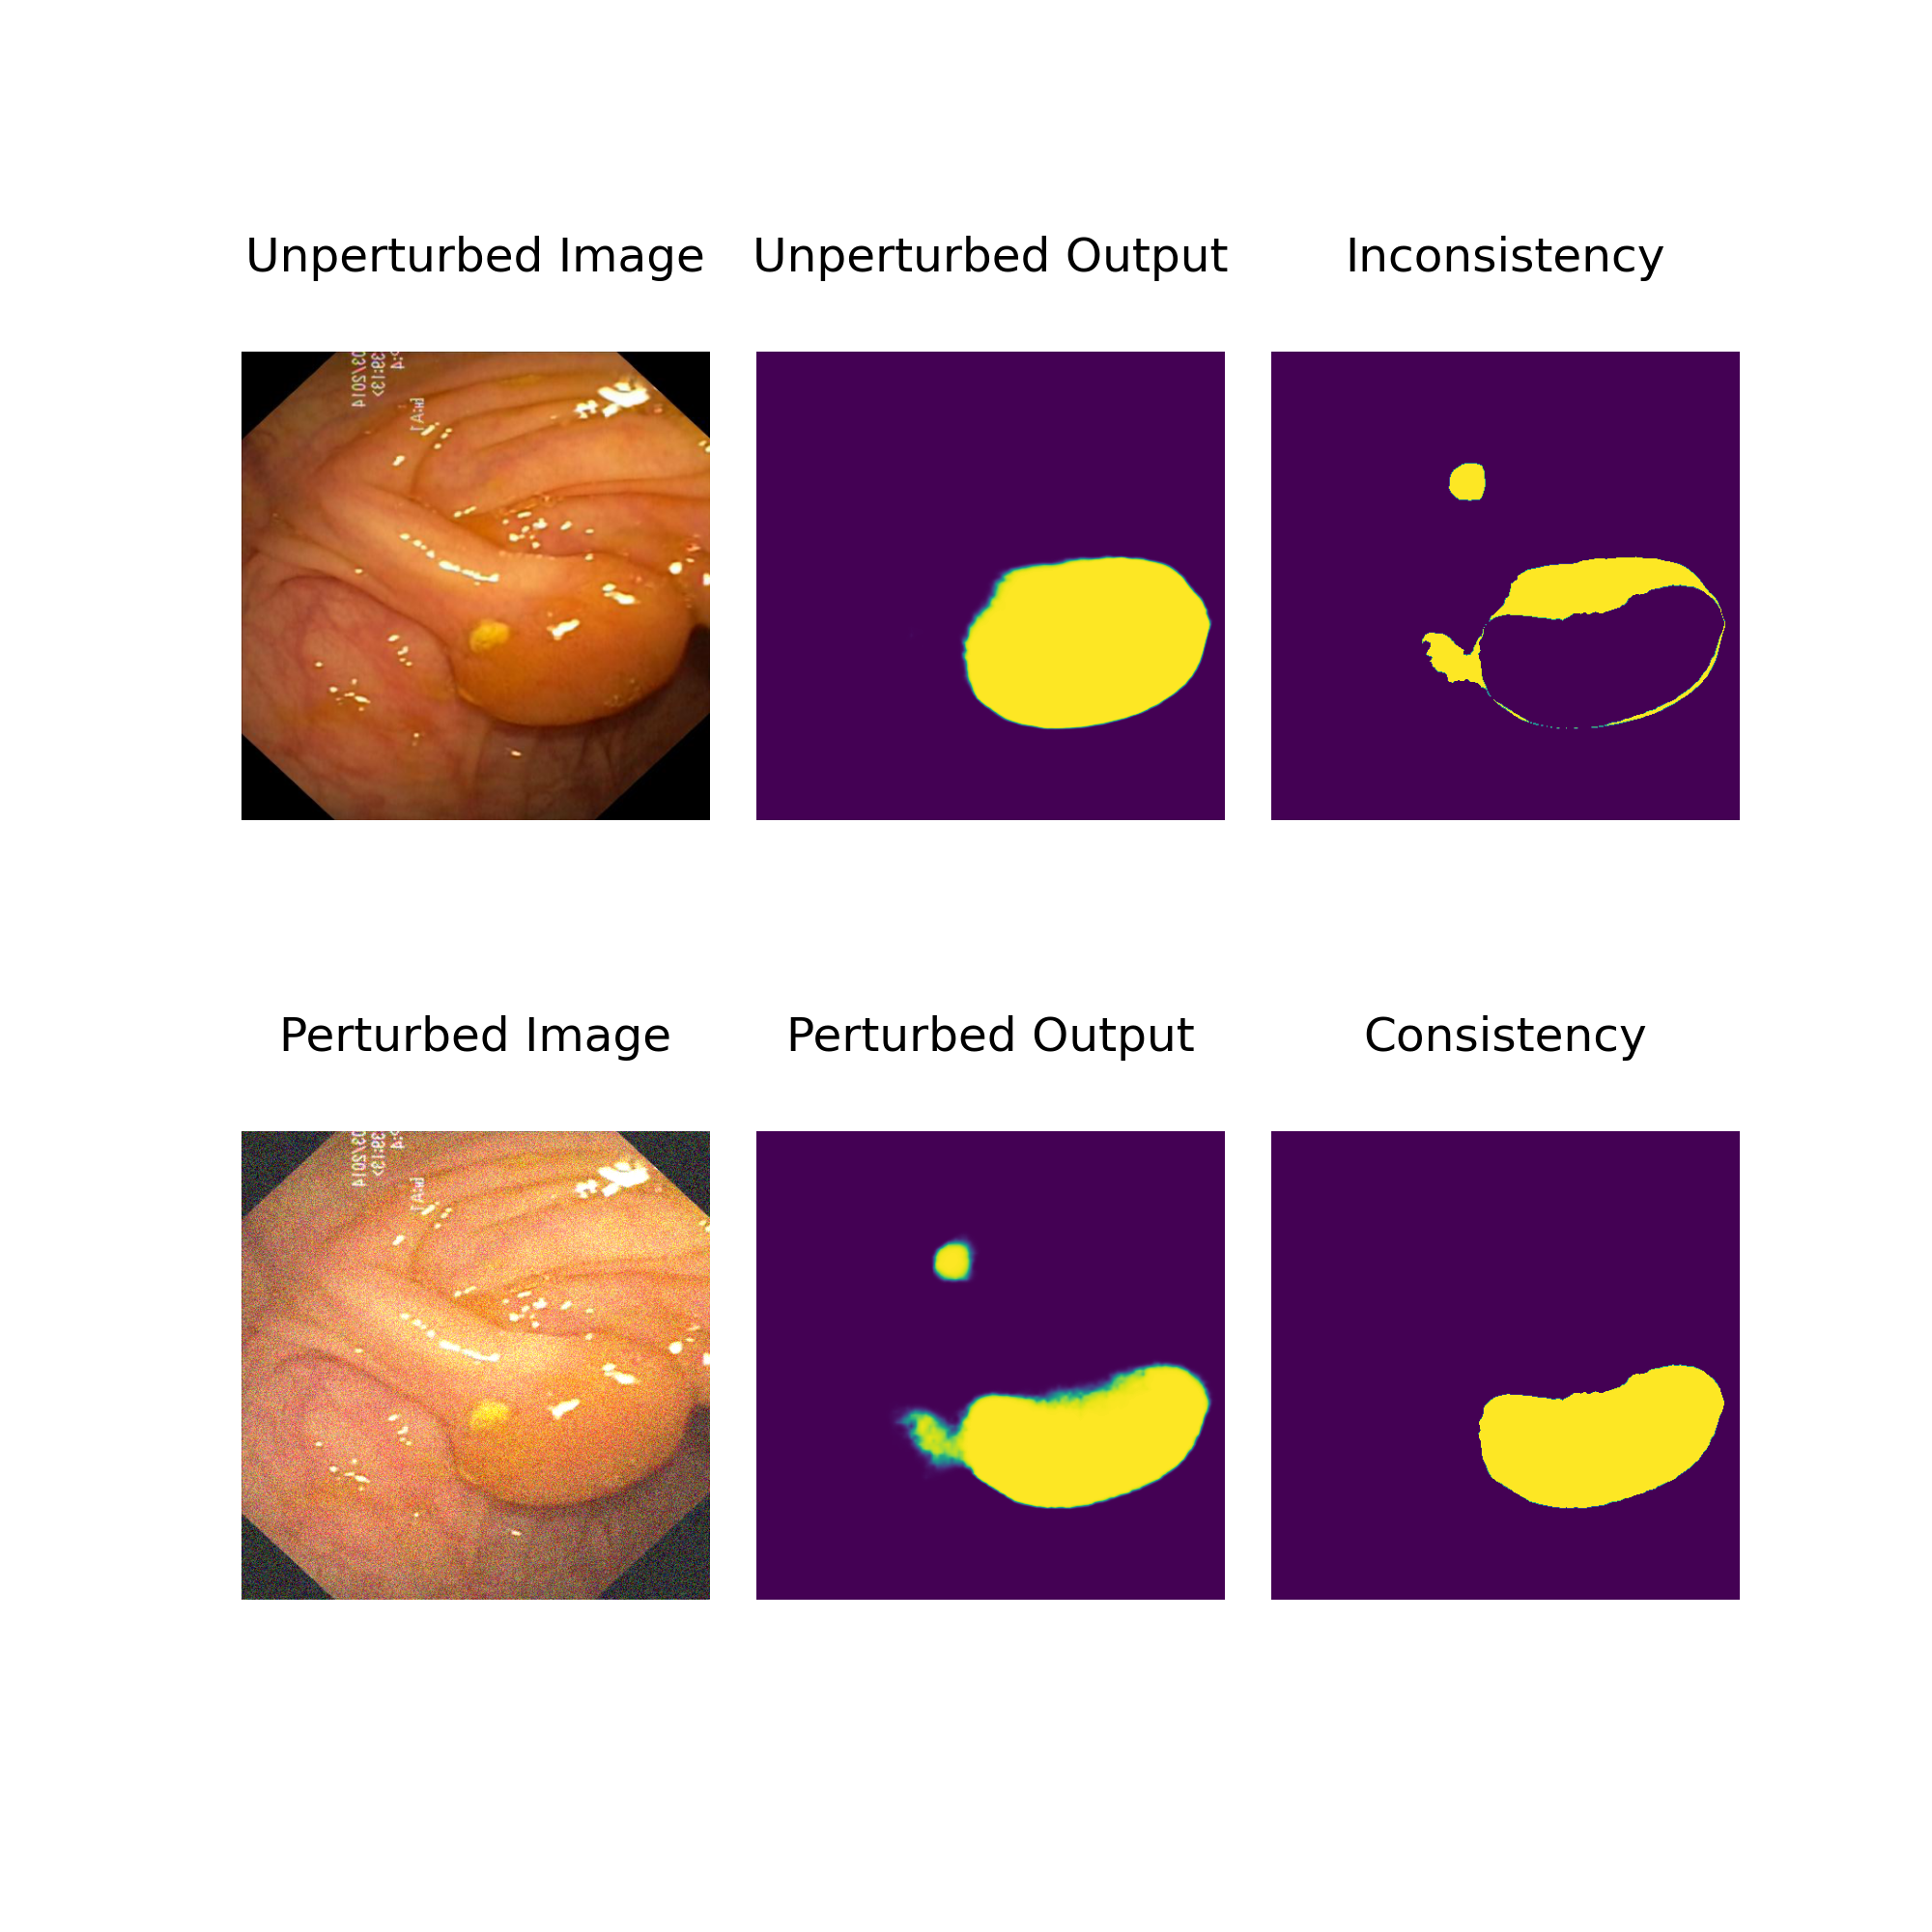
\includegraphics[width=\linewidth]{illustrations/consistency_examples.png}
    \caption[Segmentation Consistency Visualization 1]{Examples of consistency and inconsistency calculation when subjected to a non-label-altering perturbation, in this case additive noise. The consistency for this sample (when thresholded) is 0.68 and inconsistency 0.32, meaning that 64\% of the pixels constitute consistent predictions across the two inputs.}
    \label{fig:consistency_example}
\end{figure}

Using this formulation, higher is of course better. For the purpose of developing a loss function, however, it is useful to instead quantify \textit{inconsistency}. This can be expressed in much the same manner, but using the symmetric difference operator, i.e \(A \ominus B = A \cup B - A \cap B\): 
\begin{equation}\label{eq:inconsistency}
    \overline{\mathcal{C}}(A,Y) = \frac{1}{\sum\{y \cup a \cup \hat{y} \cup \hat{a} \}} \sum \{y\ominus\hat{y}\ominus a\ominus\hat{a}\}
\end{equation}
These formulations are, of course, related by:
\begin{equation*}
    \mathcal{C}(A,Y) = 1-\overline{\mathcal{C}}(A,Y)
\end{equation*}

This notion of inconsistency then corresponds to counting the number of pixels that change after the input is subjected to a perturbation - \(\hat{a}\ominus \hat{y}\), but discounting those we expect to change, \(a\ominus y\). This is also shown in ~\Cref{fig:consistency_example} and~\Cref{loss_fn}.

It is worth noting that consistency is maximized - and thus inconsistency minimized - not only if the predictions are both correct and consistent with one another, but also if the predictions are both incorrect, as long as whatever change that occurs corresponds to the expected change. This is illustrated in~\Cref{loss_fn}.
\begin{figure}[htb]
    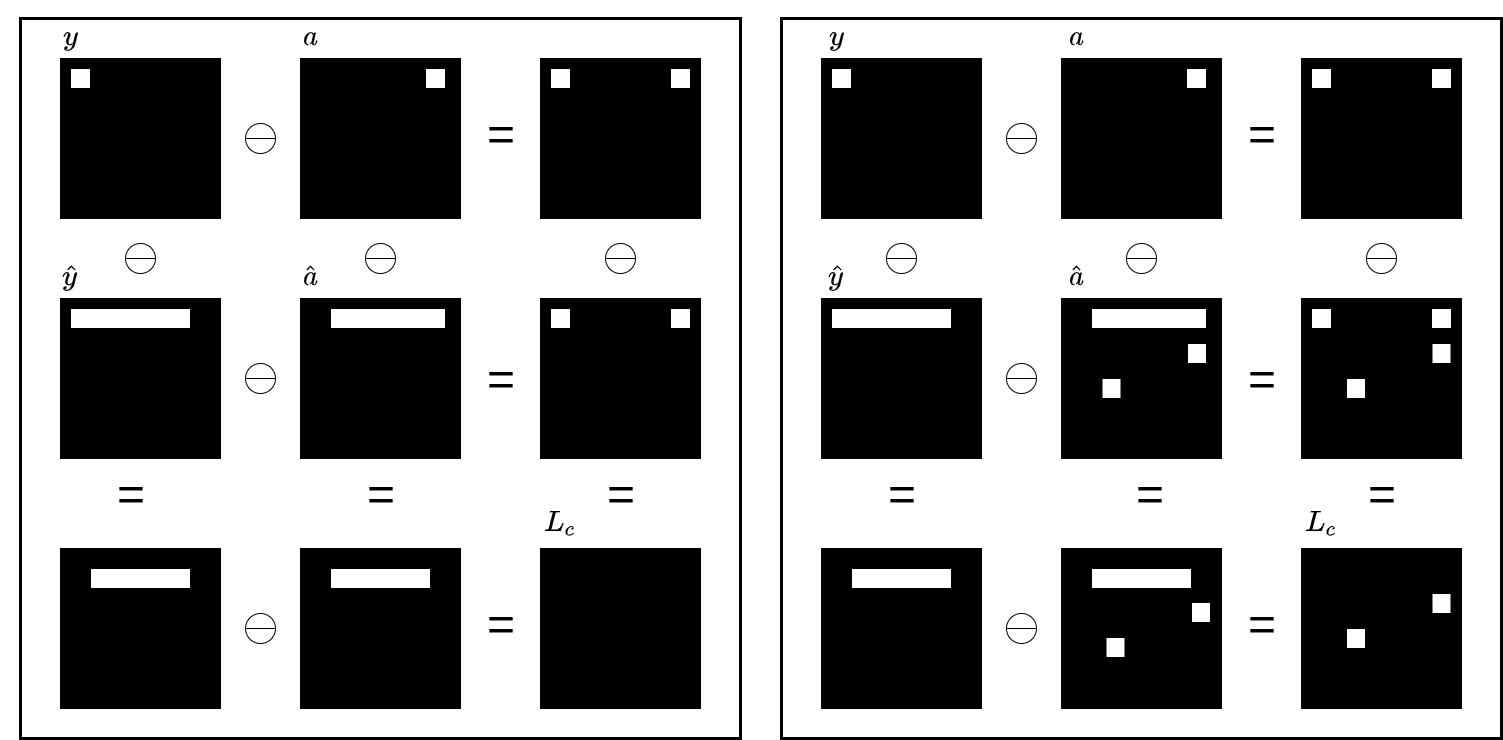
\includegraphics[width=\linewidth]{illustrations/loss_visualisation.drawio.png}
    \caption[Segmentation Consistency Visualization 2]{Visualisation of consistency calculation when subjected to a label-altering perturbation, where white is a positive prediction. Note that \(\overline{\mathcal{C}}\) is zero regardless of prediction correctness so long as it changes in the expected manner. Note also that the symmetric difference operators are associative. Left shows an instance of consistent and partially incorrect predictions, and right shows an instance of inconsistent and partially correct predictions.}
    \label{loss_fn}
\end{figure}  
    
Moreover, note that this metric does not presuppose what transformation has occurred. In~\Cref{loss_fn}, for instance, the change induced by the perturbation may correspond to simply moving the polyp in the image (and replacing the empty space with a believable background), or it may correspond to a rotation by 90 degrees. How this should be analyzed with respect to consistency is up to interpretation - one can argue that a rotation should rotate the incorrect predictions as well, or one can argue that it should only rotate the correct component of the prediction. For simplicity, Consistency Training is based on the latter interpretation. This will be discussed in further detail in~\Cref{conclusion}.

\subsection{Inconsistency Loss}
Inconsistency as expressed in~\Cref{eq:inconsistency} is not differentiable, and thus it cannot in its current state be used as a part of a loss function. This, naturally, limits the utility of the idea somewhat. Thus, a smooth extension of this metric is needed which can be achieved in much the same way as how the Jaccard loss can be derived from the Jaccard index - i.e by using differentiable versions of the set functions. 

We can extend the definition of the symmetric difference to \(\Theta(A,B) = A(1-B) + B(1-A)\). This, naturally, is equivalent to the standard symmetric difference if the values of A and B are binary. Similarly, the union operator can be extended as \( \bigcup(A,B) = A+B-AB\), and the intersection operator as \( \bigcap(A,B) = AB\). Like its binary equivalents, these operators maintain their associative and commutative properties. One can optimize for consistency by replacing the operators in~\Cref{eq:inconsistency} with these functions, which in turn can be used as a loss function:

\begin{equation}
    L_c(y, \hat{y},  a, \hat{a}) = \sum \frac{\Theta(y, \hat{y},  a, \hat{a})}{\bigcup(y, \hat{y},  a, \hat{a})}
\end{equation}

This loss function will from this point be referred to as the \gls{sil}. 

\subsection{Adaptive Loss Weighing}
    Naturally, using \gls{sil} as a loss function on its own is not really useful since it only expresses inconsistency, and is to a large extent agnostic to whatever object it is trying to segment. For instance, if the perturbation being performed is simply additive noise, the loss is equally well minimized by predicting that every pixel is positive as it is by segmenting the polyps alone. Consequently, it has to be combined with a some conventional segmentation loss, for instance Jaccard loss. A simple way to do this would be to simply add them together and normalize, i.e:
\begin{equation*}
    L(Y, A) = \frac{1}{2} \big[L_{seg}(Y)+L_c(Y,A)\big]
\end{equation*}
Preliminary experiments showed that this, however, exhibited some degree of instability. The model would readily get stuck in local minima where its predictions were indeed consistent, but also consistently predicting artifacts. Examples of this can be found in~\Cref{non_weighted_ctraining}. 

To mitigate this, it is possible to employ a weighing strategy. Instead of simply adding the respective losses together, one may weight the individual components adaptively according to the \gls{ind} segmentation performance. This way, the model will learn to predict generally correct segmentations early in the training, then start weighing consistency and as a result generalization more and more as the model sees improvements to its segmentation performance:
    \begin{equation}
        L = (1-IoU)\times L_{seg} + IoU \times L_c
    \end{equation}
Using this formulation, the model will start off trying to learn features that contribute to generally improved segmentation performance, then as segmentation performance improves start principally focusing on learning to be consistent. If the model starts veering into areas in the loss-landscape that constitute poor segmentation performance, it will self-correct by weighing the segmentation loss more. In the implementation used in this thesis, these \gls{iou} weights were calculated on a per-batch basis such that the model can quickly adapt if either of the respective objectives exhibit a degradation in performance during training. 

\subsection{Conventional Data Augmentation and Consistency Training}\label{cons_vs_aug}
    At this point, one may easily make the argument that Consistency Training is merely a somewhat more elaborate form of regular data augmentation. To some extent, this argument is well-founded; data augmentations are after all a form of perturbation, and one may argue that \gls{erm} is the mechanism by which consistency across these perturbations is minimized. There are, however, a number of nuances that separate the two methods, as will be discussed below and elaborated upon through mathematical analysis in~\Cref{discussion}. 
    
    With conventional data augmentation, one might assume that the model learns to be invariant to the augmentations as a byproduct of minimizing the empirical risk. By extension, it is assumed that the model will learn features that are equally performant across augmentations. After all, the risk-minimizing configuration is in this case that which exhibits the highest degree of performance when averaged across both augmented and non-augmented images. 
    
    This, however, is not necessarily the case. To illustrate, consider a pipeline intended to segment melanomas. As mentioned in~\Cref{gen_failure_med}, the models in such pipelines are often sensitive to skin-tone. Let us assume that the dataset consists primarily of patients with light complexions, and that data augmentation is used in an attempt to combat any bias as a result of this unbalanced dataset. For simplicity, let us assume that the only augmentation used is transforming the image with colour-jitter with probability \(p=0.5\). In theory, the empirical risk will be best minimized by learning features that do not consider colour and thus skin-tone at all, and instead simply learn to consider the shapes and sizes of the melanomas, the irregularity of which is typically considered a the principal hall-mark of melanomas. 
    
    This is unlikely for two reasons: first, it presupposes that the model readily learns these generalizable features in favor of the more predictive but spurious features during gradient decent. Second, it assumes that learning to perform well is equally easy on both the augmented and the un-augmented images. If, for instance, the model can quickly achieve high average performance and thus minimize risk locally by using color features to achieve excellent performance on the non-augmented images, while exhibiting mediocre or even poor performance on the augmented data, it is unlikely that the model will ever exit this extremely broad local minimum in favor of a more shape-biased and generalizable configuration. Moreover, it may be the case that these shape-based features require significantly more parameters in order to be able to model sufficiently and thus that the performance on the augmented data is limited to a much lower upper bound. In this case, the risk will be minimized not by learning features invariant to the transform, but by learning features that result in a sufficient equilibrium of performance across the augmented and unaugmented sets. I.e, it will try to learn predictive but brittle features as much as possible to maximize performance on unaugmented data, but under the condition that the performance does not degrade too much on the augmented data. Consistency training mitigates this by quantifying the inconsistency of the predictor subject to perturbations, and directly minimizing this quantity. Moreover, due to the weighing method used, consistency is also prioritized starting fairly early in gradient descent. 
    
    Thus, though the two methods share similar traits, they are distinct. Consistency Training can however as mentioned in~\Cref{introduction} be considered an alternative to conventional data augmentation; in pipelines wherein data augmentation is used, one can implement Consistency Training instead so long as there is a suitable method by which to quantify inconsistency. 

\subsection{Putting it all together}
To summarize, Consistency Training is based on the idea that a model necessarily must have learned generalizable features if it has learned invariance to all possible perturbations that do not affect the causal structure of the problem. This is achieved using a perturbation model \(\epsilon(\cdot)\), and a loss function which quantifies the inconsistency of the model when subjected to this perturbation. This loss term then has to be incorporated into the final loss function along with a task-specific loss, hence the adaptive loss weighing. The overall algorithm training process is shown in~\Cref{alg:consistency}:
\begin{algorithm}[htb]
    \caption{Consistency Training}\label{alg:consistency}
    \begin{algorithmic}
    \For{$epochs$}
        \For{$\left(batched\right) {x,y} \in dataset$}
        \State $x_a, a = \epsilon(x, y)$
        \State $\hat{y} \gets f(x)$
        \State $\hat{a} \gets f(x_a)$
        \State $\Bar{\mathcal{C}} \gets \frac{\Theta(\hat{x}, \hat{a},x,a)}{\bigcup(\hat{x}, \hat{a},x,a)}$
        \State $k \gets IoU(x,y)$
        \State $\mathcal{L} = (1-k) \mathcal{J}(x,y) + k \Bar{\mathcal{C}}$
        \State $f(\cdot) \gets optimizer\_update(\mathcal{L})$
        \EndFor
    \EndFor
    \end{algorithmic}
\end{algorithm}


\section{Consistency-trained Ensemble Models}
As mentioned in~\Cref{background}, ensemble-based models have demonstrated high degrees of generalizability~\cite{divergentnets, endoensemble}. Assembling predictors trained with Consistency Training into an ensemble is as a result a simple but effective means by which generalizability can be further increased. 

This can be achieved fairly simply by leveraging multiple identically trained models, such as the dual-decoder DeepLabV3+ - or indeed any model, as will be demonstrated in~\Cref{experiments}. These models can then be used to generate a unique segmentation probability map for each model. This can then be combined into a heatmap, which can then in turn be used to facilitate prediction through the use of any number of consensus methods. In this thesis, the ensembles were implemented to predict according to a simple majority-vote, i.e by thresholding the probability heatmap such that all pixels with probabilities above 0.5 were considered as positive predictions. This is illustrated in~\Cref{fig:ensemble_setup}.

\begin{figure}[htb]
    \centering
    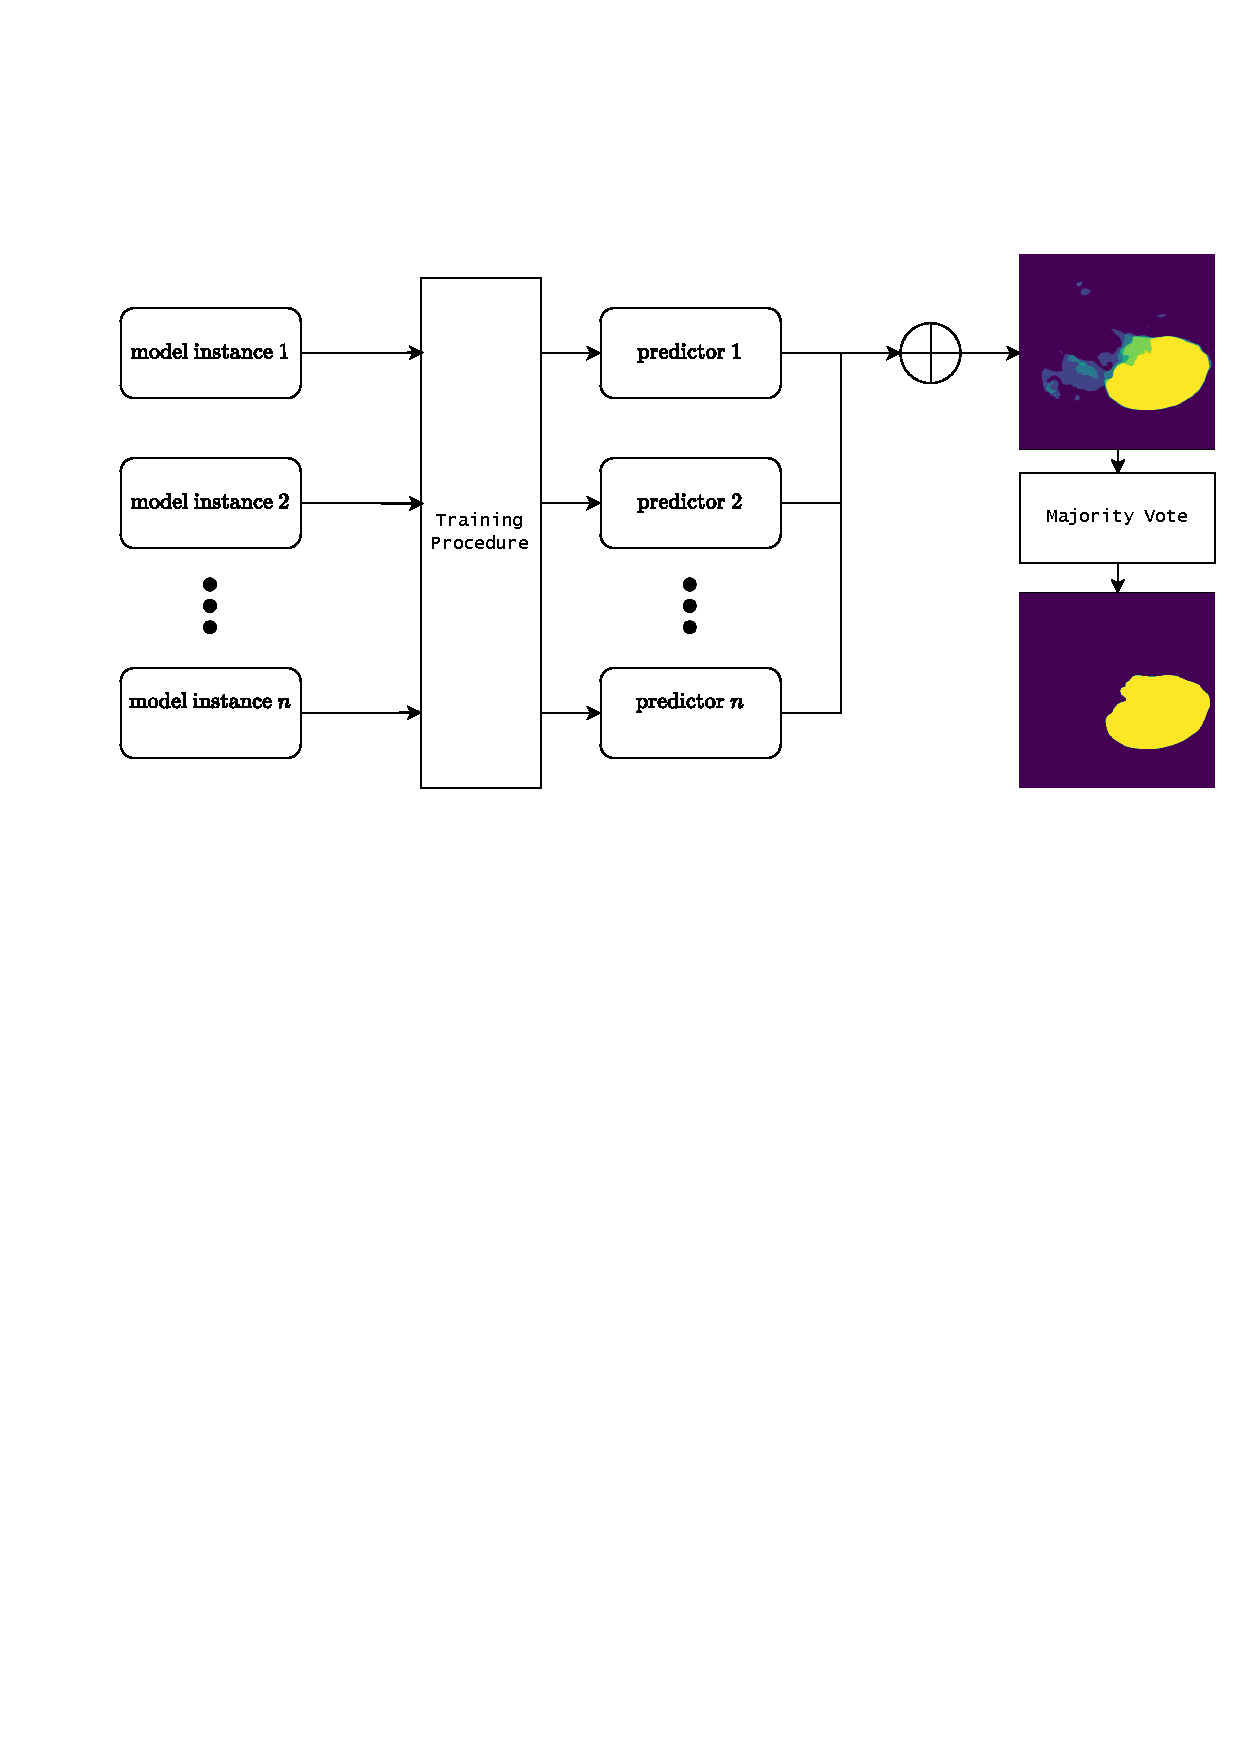
\includegraphics[trim=1.5cm 16cm 0cm 4cm, clip, width=\linewidth]{illustrations/ensemble_config.pdf}
    \caption{Implementation of Ensembles}
    \label{fig:ensemble_setup}
\end{figure}

As mentioned in~\Cref{background}, ensemble models can be considered a form of Bayesian marginalization. As a result, the model is less likely to be affected by underspecification by virtue of the fact that whatever variability in the space of features that a predictor can learn is to some extent accounted for.  

\section{Summary}
This chapter has covered the implementation and theoretical basis for the methods introduced in this thesis. The \textbf{dual decoder DeepLabV3+} aims to increase generalization by constraining the models' latent feature space through the use of image reconstruction as an auxiliary task. \textbf{Consistency training} aims to increase generalization by explicitly optimizing for consistent predictions across perturbed and un-perturbed inputs. These perturbations are application-dependent, and are in this thesis implemented as a carefully designed set of augmentations, consisting of conventional image transformations and a generative inpainting model. Finally, an \textbf{ensemble model} is implemented by combining multiple dual-decoder DeepLabV3+ models trained with Consistency Training. 
    \chapter{Experiments and Results}\label{experiments}
This chapter presents the experiments conducted to evaluate the methods presented in~\Cref{methods}, as well as their set up and the experimental methodology used. The results of each experiment are then presented and discussed in brief.~\Cref{exp_meth} will present the experimental setup used in this thesis, including the choices of metrics, datasets, models used throughout all of the experiments. Baseline generalizability metrics are then collected in~\Cref{models}. The impact of data augmentation on generalization is then tested in~\Cref{augmentations}, which in turn is used as a basis for the experiments performed in~\Cref{consistency_training}, wherein the best augmentation method was selected for use in Consistency Training. Finally, the impact of ensembles is tested in~\Cref{ensembles}. All experiments where conducted using Nvidia Tesla-V100 GPUs on the eX3 computing infrastructure offered by Simula Research Laboratory. The experiments were implemented in Python 3.8 using PyTorch. The source code as well as all of the raw data is available on the GitHub repository given in~\Cref{code_data}.

\section{Experimental Setup}\label{exp_meth}
The experiments conducted in this chapter were partially exploratory and partially quantitative in nature. In addition to exploring the impact of the methods as outlined in~\Cref{methods}, the effects of more well-known methods were also compared. In particular, the effect of the choice of model architecture, the use of data augmentation, and ensemble models were quantified. This was then in turn compared quantitatively to the impact due to the methods presented in this thesis. 

Statistical significance was established using two-tailed independent-sample t-tests when comparing samples of identical models and datasets, as the resulting distribution can be considered approximately normal. In cases where this was not the case, i.e when comparing performance across all models, in which case the distribution is typically multimodal, a Mann-Whitney U-test was used. Results with p-values under 0.01 were considered significant. 

The following sections will further detail the experimental setup, including the choices of metrics, datasets, and the choice of models with which the impact of the presented methods were established. 

\subsection{Metrics and Evaluation} \label{metrics}
    This subsection will present the metrics and datasets used in order to evaluate the generalizability of the predictors presented in this thesis.  

    \subsubsection{Datasets} \label{datasets}
    Naturally, the best way to evaluate the generalizability of a given predictor is to test it directly on \gls{ood} data. Though this can to some extent be achieved by carefully designing stress-tests ~\cite{damour2020underspecification}, a more straight-forward approach is to simply leverage existing \gls{ood} datasets. To this end, a number of polyp-segmentation datasets were selected. The names, sizes, resolutions and availabilities of these datasets is shown in~\Cref{tab:datasets}. Samples images and masks from the datasets can be seen in~\Cref{fig:dataset_examples}
    
    \begin{table}[htb]
        \centering
       \begin{tabularx}{\linewidth}{lXXX}
        \toprule
        Dataset & Resolution & Size & Availability \\
        \midrule
        Kvasir-SEG ~\cite{kvasir} & Variable & 1000 & Public \\
        Etis-LaribDB ~\cite{etis-larib} & 1255x966 & 196  & Public \\
        CVC-ClinicDB ~\cite{cvc-clinic} & 388x288 & 612  & Public \\
        EndoCV2020 ~\cite{endocv2020} & Variable & 127  & Request \\
        \bottomrule
    \end{tabularx}
        \caption{Dataset Overview}
        \label{tab:datasets}
    \end{table}
    
    \begin{figure}[htb]
        \centering
        \includegraphics[width=\linewidth]{illustrations/dataset_samples.png}
        \caption{Sample images from the datasets.}
        \label{fig:dataset_examples}
    \end{figure}
    
    Ideally, the datasets used in EndoCV2021 ~\cite{endocv2021} should also have been included to facilitate for direct comparison to the results published in the EndoCV2021 proceedings, however since they were not available - neither publically nor by request - at the time of writing this thesis, this was, unfortunately, not possible. 
    
    Kvasir-SEG was selected for being used as the \gls{ind} dataset across all experiments due to its size and the diversity of images. This was then split into a training, validation and test-set, which remained constant across all experiments. The remaining datasets were used solely for \gls{ood} evaluation.
    
    All images were resized to 512x512 as preprocessing during all training runs, as some of the models required base-2 dimensionality.
    
    \subsubsection{Mean Intersection-over-Union}
    
    The most natural way to quantify generalizability is to simply evaluate the predictors on in-distribution and out-of-distribution data and then consider the differences. There are, naturally, several performance measures that can be used to this end in the context of segmentation, the most natural of which being \gls{iou} or the Dice coefficient, which as discussed in Chapter \ref{background} are equivalent. In this thesis, \gls{iou} was used. To reiterate, IoU is defined as follows:
    Let \(y\) be the segmentation label, and \(\hat{y}=f(x)\) be the segmentation prediction given the model \(f\) and an input image x. The \gls{iou} can then be expressed as: 
    \begin{equation*}
        IoU(y, \hat{y}) = \frac{\sum \{y=\hat{y}\} }{\sum \{y=1\} \cup \{\hat{y}=1\}\}}
    \end{equation*}
    
    Measuring the average \gls{iou} scores across a number of different datasets should, naturally, provide an indication of the generalizability of the given predictor. Though it is of course impossible to account for all distributional shifts that may occur in deployment, high degrees of generalization across multiple datasets should nevertheless translate well to other datasets. 

    
    \subsubsection{Performance Variability}
    As discussed in~\Cref{background}, the prevalence of generalization failure is often attributed to the notion of underspecification. Underspeficified pipelines are characterized by the fact that they can return any number of different predictors, which though all exhibiting more or less identical performance in \gls{ind} settings, learn differing and often conflicting features and thus may differ wildly in \gls{ood} settings. 
    
    To analyze this, the literature tends to consider the performance variability of a set of multiple identically trained predictors ~\cite{damour2020underspecification}.  
    
    One simple approach to quantify this is to take the standard deviation of the mean \gls{iou} scores for the given datasets and predictors. This, however, implicitly rewards predictors that perform poorly. To mitigate this, the \gls{cs} can instead be used. \gls{cs} is similar to the standard deviation, but normalized by the mean:
    \begin{equation}
        C.StD = \frac{1}{n \mu} \sqrt{ \sum_i^n (\mu - x_i)^2  }
    \end{equation}
    
     Though the mean generalizability gap across these predictors is the primary indication of generalizability of the pipeline, this variability is also a salient factor to consider as it serves to quantify the degree to which a given pipeline is underspecified. The more underspecified a pipeline is, the higher the variability of the performance and the higher the \gls{cs} of the \glspl{iou}.  

\subsection{Models} \label{model_choices}
In order to evaluate the impact of the methods presented in~\Cref{methods} sufficiently, they need to be tested across a range of different models. This ensures that the effects induced my the methods are not model-dependent, and in addition provides an opportunity to investigate the innate ability of specific models to learn generalizable features. To this end, a number of popular models were selected, intended to serve as a somewhat representative sample of what may be considered as "typical" deep learning pipelines. These models include DeepLabV3+ ~\cite{deeplab}, \gls{fpn} ~\cite{fpn}, UNet ~\cite{unet}, Tri-Unet ~\cite{divergentnets}, and the dual-decoder DeepLabV3+ as introduced in Chapter \ref{methods}. 

The models were implemented in pytorch using the segmentation-models-pytorch (SMP) library ~\cite{smp}, using the library's default values.~\Cref{tab:baselines} shows the architecture type and parameter counts of the respective models. 
  \begin{table}[htb]
            \centering
            \begin{tabularx}{\linewidth}{lXr}
            \toprule
                 Model & Architecture & Parameters  \\
            \midrule
                 UNet ~\cite{unet} & Encoder-Decoder & 48872738\\ 
                 TriUnet ~\cite{divergentnets}
                 Stacked Encoder-Decoder & 122178709\\
                 FPN ~\cite{fpn} & Pyramidal & 47591762\\ 
                 DeepLabV3+ ~\cite{deeplab} & Hybrid & 22437457\\ 
                 Dual Decoder DeepLabV3+& Single-encoder Dual-decoder & 23590756\\
            \bottomrule
            \end{tabularx}
            \caption{Experiment Models}
            \label{tab:baselines}
        \end{table}
The models were all intialized using SMP's built-in pretrained weights, trained on ImageNet. Though foregoing pretraining would perhaps highlight the respective models' innate generalization ability to a greater extent, the use of pretrained weights nonetheless constitutes a more realistic context, as most computer vision pipelines, especially those of a medical nature, employ some form of pretraining. As will be discussed in~\Cref{discussion}, evaluating the generalizability of different models without pretraining may however be an interesting direction of further study. 
 

\section{Model Architecture} \label{models}
To establish the effect of model architectures alone, ten predictors were trained for each model without augmentation and using regular Jaccard loss, according to the hyperparameters shown in~\Cref{table:hyperparameters}. 
\begin{table}[htb]
        \centering
        \begin{tabularx}{\linewidth}{llX}
        \toprule
        \multicolumn{3}{c}{\textbf{Pipeline Configuration}}\\
        \toprule
        Component & Type & Hyperparameters \\
        \midrule
        Dataloader & - & \(batch\_size = 8\) \\
        && \(\hbox{train/val/test split} = 80/10/10\)\\
        \midrule
        Optimizer & Adam & \(lr = 0.00001\)\\
        \midrule
        Scheduler & Cosine Annealing w/ Warm Restarts & \(T_0=50\) \\
        & & \(T_{mult}=2\) \\
        \midrule
        Evaluation & Loss-based Early Stopping & \(epochs=300\)\\
        \bottomrule
        \end{tabularx}
            \caption{Hyperparameters for baselines}
            \label{table:hyperparameters}
\end{table}

The \gls{ood} \glspl{iou} are shown in~\Cref{tab:baseline_iou}. The numerical precision has been truncated to the 99\% confidence interval. Though the differences between many pairs of models are statistically significant for several datasets, the magnitude thereof is marginal to the point of being inconsequential for practical purposes, with the exception of TriUnet which exhibited considerably worse generalization. All p-values are shown in~\Cref{models_pvalues} in Appendix A.

\begin{table}[htb]
    \centering
    \small
    \begin{tabularx}{\linewidth}{@{}lXXXX@{}}
    \toprule
    & Kvasir-SEG & Etis-LaribDB & CVC-ClinicDB & EndoCV2020 \\
    \midrule
    DeepLabV3+ & 0.819 & \textbf{0.412}  & 0.678 & 0.604 \\
    DD-DeepLabV3+ &\textbf{0.832} & 0.406 & \textbf{0.683} & 0.595 \\
    Unet & 0.828 & 0.403 & 0.679 & 0.599 \\
    TriUnet & 0.822 & 0.305 & 0.633 & 0.581 \\
    FPN& 0.823 & 0.404 &0.678 & \textbf{0.605}\\
    \bottomrule
    \end{tabularx}
.    \caption[Mean IoU scores for each model across datasets]{Mean IoU scores for each model across datasets. The best models for each dataset are highlighted in bold.}
    \label{tab:baseline_iou}
\end{table}

\Cref{fig:baseline_ious} shows the models' average change in mean \gls{iou} across the three \gls{ood} datasets with respect to the mean \gls{iou} of the \gls{ind} dataset. All models exhibited considerable performance degradation, and as before the differences across architectures are insignificant, once again with the exception of the TriUnet. 
    \begin{figure}[htb]
        \centering
        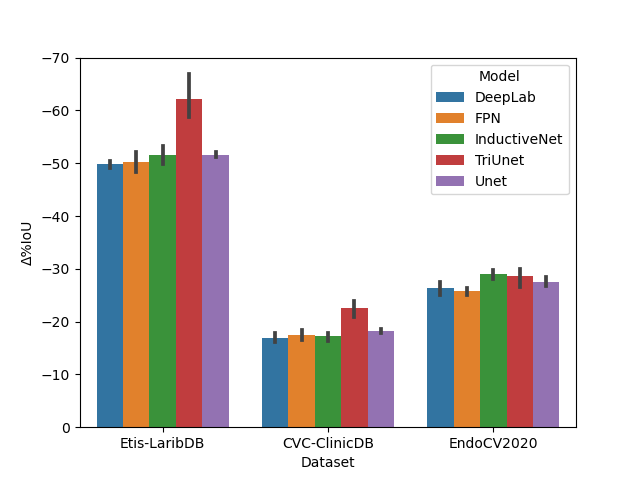
\includegraphics[width=\linewidth]{illustrations/delta_iou_baseline.png}
        \caption{Change in \gls{ood} \gls{iou} as a percentage of the \gls{ind} \gls{iou} across models and datasets.}
        \label{fig:baseline_ious}
    \end{figure}

    What differences there are across the models, however, can be understood according to their relationship with underspecification.~\Cref{fig:baseline_cstd} shows the \gls{cs} values for each model and dataset as computed from the evaluation of the ten predictors. Of particular interest is the relationship between the Unet and the TriUNet, as well as DeepLabV3+ and the dual-decoder counterpart. The differences between these two pairs of models will be discussed in further depth below.
    
    \begin{figure}[htb]
        \centering
        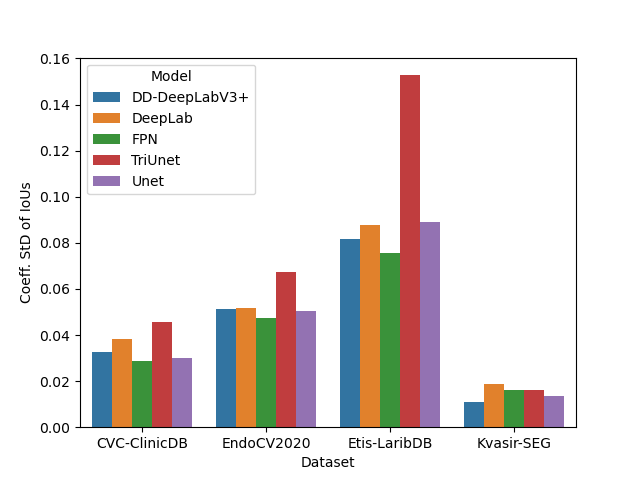
\includegraphics[width=\linewidth]{illustrations/cstd_baseline.png}
        \caption{Coefficient of Standard Deviation across models and datasets.}
        \label{fig:baseline_cstd}
    \end{figure}
    
    \subsubsection{Unet vs TriUnet}
    Consider the TriUnet and how its variability is higher and \gls{ood} performance lower compared to the regular Unet. As the TriUnet consists of three UNets, conventional analyses would assert that the TriUnet should exhibit equivalent performance or greater. However, the results instead demonstrate that the TriUnet on average performs worse than the regular Unet as well as exhibiting significantly higher performance variability. This corroborates the notion that underspecification plays a significant role in generalization failure; the TriUnet is highly underspecified in comparison to the Unet, as the difference in performance variability between shows in~\Cref{fig:baseline_cstd}.
    
    \subsection{DeepLabV3+ vs DD-DeepLabV3+} \label{dd-deeplab}
    DeepLabV3+ and DD-DeepLabV3+ both exhibited more or less comparable performance when considering their \gls{ood} IoUs, as shown in~\Cref{tab:baseline_iou}. Interestingly, though, the dual-decoder model performed better on the \gls{ind} dataset - Kvasir-Seg - by a statistically significant margin (p<0.01). There are also some differences with regards performance variability, albeit minor. As shown in~\Cref{fig:baseline_cstd}, the DD-DeepLabV3+ exhibits lower \gls{cs} scores than its single-decoder counterpart. Since the models are as mentioned functionally identical except for the presence of the reconstruction decoder during the training of DD-DeepLabV3+, this can only be attributed to the model learning a more limited latent representation and thus being less underspecified. 
    
    \begin{figure}[htb]
        \centering
        \includegraphics[width=\linewidth]{illustrations/reconstruction_samples.png}
        \caption{Reconstruction Examples across datasets}
        \label{fig:reconstruction}
    \end{figure}

    The differences between the two models are smaller than expected, however. One possible explanation for this may be that segmentation encoders learn somewhat task-agnostic representations of the data by default, and that the presence of a reconstruction decoder merely refines these representations to a minor extent, however in a manner that does not meaningfully affect the segmentation task. This notion is supported by the fact that the reconstruction seems to be equally good in terms of L1-distance across all four datasets. If the encoder had learned dataset-specific features, this would not be the case. A histogram showing the distribution of L1-scores across the four dataset is shown in~\Cref{fig:l1_rec}. Reconstruction examples are shown in~\Cref{fig:reconstruction}. Most of the errors seem to cluster around areas of high reflectivity regardless of dataset.  
    
    \begin{figure}[htb]
        \centering
        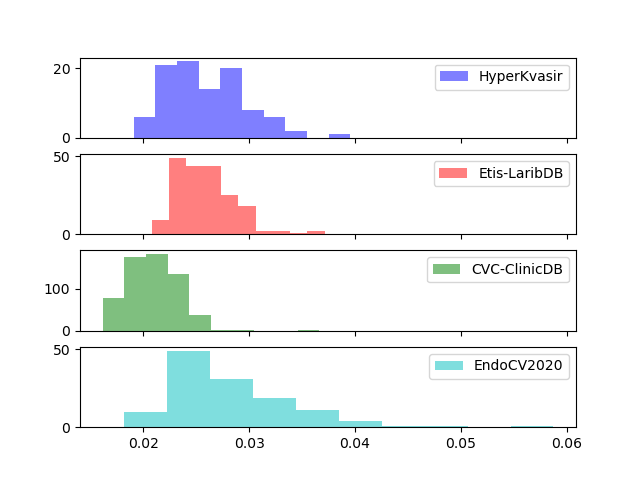
\includegraphics[width=\linewidth]{illustrations/l1_reconstruction.png}
        \caption[L1 reconstruction distributions across datasets]{Distribution of L1 reconstruction scores across datasets. Though the distributions vary, there is no clear evidence of generalization failure in terms of reconstruction.}
        \label{fig:l1_rec}
    \end{figure}
    

\section{Augmentation Strategies}\label{augmentations}
The baseline predictors collected in the previous section were then compared to predictors trained using data augmentation. Two augmentation strategies were tested: one with conventional augmentations only, while the other also incorporates the GAN-inpainter. The models were trained according to the same hyperparameters as described in~\Cref{table:hyperparameters}. The data augmentation strategy was implemented using the albumentations library, and the hyperparameters were tuned according to the methods referred to in~\Cref{methods}. The data was then augmented with a probability of 0.5, in which case the constituent transformations were applied according to the ranges defined by the hyperparameters. The results for each configuration and across models and datasets are shown in~\Cref{tab:aug_ious}.

\begin{table}[htb]
    \centering
\begin{tabularx}{\linewidth}{lXXX}
\toprule
Model & No Augmentation & Vanilla Augmentation & Inpainter+Vanilla Augmentation\\
\midrule
\multicolumn{4}{c}{\textbf{Kvasir-SEG }}\\
\midrule
           DD-DeepLabV3+     & 0.829 & \textbf{0.848} & 0.844\\
           DeepLabV3+        & 0.822 & \textbf{0.850} & 0.846\\
           FPN               & 0.822 & \textbf{0.853} & 0.848\\
           TriUnet           & 0.817 & 0.841          & \textbf{0.842}\\
           Unet              & 0.828 & \textbf{0.851} & 0.846\\
\midrule
\multicolumn{4}{c}{\textbf{Etis-LaribDB}}\\
\midrule
           DD-DeepLabV3+     & 0.408 & \textbf{0.460} & 0.435\\
           DeepLabV3+        & 0.417 & \textbf{0.472} & 0.451\\
           FPN               & 0.404 & \textbf{0.440} & 0.422\\
           TriUnet           & 0.309 & \textbf{0.410} & 0.382\\
           Unet              & 0.403 & \textbf{0.447} & 0.414\\
\midrule
\multicolumn{4}{c}{\textbf{CVC-ClinicDB}}\\
\midrule

           DD-DeepLabV3+     & 0.681 & \textbf{0.728} & 0.713\\
           DeepLabV3+        & 0.684 & \textbf{0.733} & 0.718\\
           FPN               & 0.675 & \textbf{0.715} & 0.705\\
           TriUnet           & 0.623 & \textbf{0.684} & 0.659\\
           Unet              & 0.679 & \textbf{0.717} & 0.703\\
\midrule
\multicolumn{4}{c}{\textbf{EndoCV2020}}\\
\midrule
           DD-DeepLabV3+     & 0.596 & \textbf{0.668} & \textbf{0.668}\\
           DeepLabV3+        & 0.608 & \textbf{0.676} & 0.670\\
           FPN               & 0.600 & \textbf{0.662} & 0.661\\
           TriUnet           & 0.577 & \textbf{0.667} & 0.656\\
           Unet              & 0.598 & 0.660          & \textbf{0.665}\\
\bottomrule
\end{tabularx}
    \caption[Mean IoUs across augmentation strategies grouped by model and dataset.]{Mean IoUs across augmentation strategies grouped by model and dataset. The best augmentation strategy for each dataset and model are highlighted in bold. }
    \label{tab:aug_ious}
\end{table}

Both augmentation strategies exhibit an increase in \gls{ood} performance when compared to the baseline, i.e no augmentation (p<0.01). Averaged across models, the predictors trained using both conventional augmentations and the inpainter perform worse than the predictors trained with the conventional augmentations only on Etis-LaribDB and CVC-ClinicDB (p<0.01). There appear to be insignificant differences for the remaining two datasets. The p-values for each dataset can be found in~\Cref{tab:ttest_avgs_inpainter}. When considering each model individually, the differences are statistically insignificant, though this can be attributed to the low sample size. The p-values for this can be found in~\Cref{tab:ttest_per_dataset_inpainter}. 

The relative improvements due to the two augmentation strategies as a percentage of the mean \gls{iou} of the baselines is shown in~\Cref{fig:augmentations}. 

\begin{figure}[htb]
    \centering
    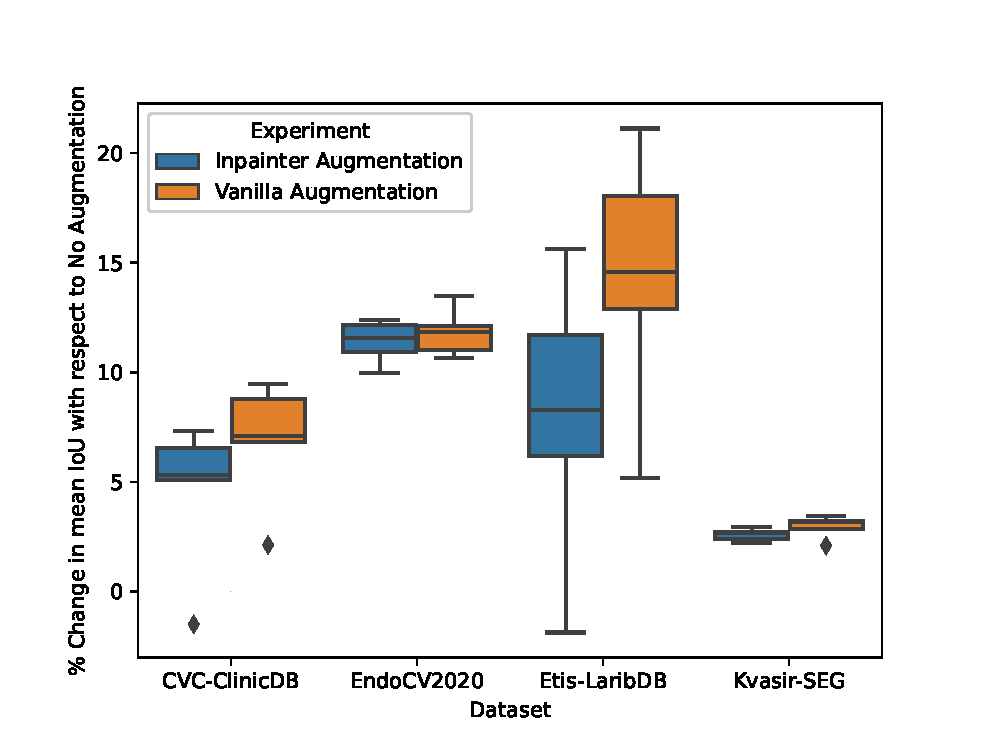
\includegraphics[width=\linewidth]{illustrations/augmentation_plot.eps}
    \caption[Augmentation Improvements]{Box plot showing the improvements in \gls{iou} per dataset as a percentage of the mean \gls{iou} for the unaugmented predictors. }
    \label{fig:augmentations}
\end{figure}

The difference between the three augmentation strategies is best highlighted by the models' performance on Etis-LaribDB, the most difficult of the three \gls{ood} datasets, which exhibits increases in mean \gls{iou} of 7.99\% using the inpainter and conventional augmentation and 14.35\% using only conventional augmentation. The differences are slightly less pronounced on the CVC-ClinicDB dataset, now with mean \gls{iou} improvements of 4.55\% AND 6.86\& respectively, and negligible on the two remaining datasets. One possible reason for this is that the inpainter may have learned \gls{ind}-specific features, and thus increase the models' bias towards learning these types of features. One can to a minor extent argue that this may explain the limited difference between the two aforementioned augmentation strategies in the \gls{ind} dataset, i.e KvasirSeg. However, it does not seem to affect the performance on the EndoCV2020 dataset by any significant margin either. One possible explanation for this is that the polyps look similar in both datasets, but verifying this requires further experimentation. 

Regardless, it is clear that synthetic augmentation as implemented in this thesis does not benefit generalization. As will be discussed in~\Cref{discussion}, however, the results do not however conclusively prove the inefficacy of \gls{ind}-trained \glspl{gan} for augmentation as a whole, only that it is unlikely that the implementation in this thesis is particularly useful. 


\section{Consistency Training}\label{consistency_training}
Though data augmentation on its own increases generalizability by virtue of the fact that it increases the support of the model, it does not explicitly impose any inductive biases, and as discussed in~\Cref{methods} may not be sufficient to impose invariance to the relevant transformations. To address this, Consistency Training was introduced. To reiterate, Consistency Training requires a perturbation model - in practical terms, an augmentation strategy - and a loss function that quantifies the degree to which the model is inconsistent to these perturbations, which for the segmentation task is implemented as \gls{sil}. In the previous section, it was established that conventional augmentations are the most conducive to generalization. Thus, this augmentation strategy was chosen as the perturbation model. 

For each model architecture, ten predictors were trained using Consistency Training, once again using the same hyperparameters as shown in~\Cref{table:hyperparameters}. This was then compared to the predictors trained using the conventional pipeline with the same augmentation strategy, as Consistency Training is as discussed in practical an alternative to conventional augmentation, and to predictors trained without augmentation. The \glspl{iou} for this experiment are shown in~\Cref{tab:aug_ious}.

\begin{table}[htb]
    \centering
\begin{tabularx}{\linewidth}{llXX}
\toprule
\textbf{Model} & \textbf{No Augmentation} & \textbf{Vanilla Augmentation} & \textbf{Consistency Training}\\
\toprule
\multicolumn{4}{c}{\textbf{Kvasir-SEG  }}\\
\midrule

        DD-DeepLabV3+& 0.829 & 0.848 & \textbf{0.852} \\
        DeepLab& 0.822 & 0.850 & \textbf{0.852} \\
        FPN& 0.822 & \textbf{0.853} & 0.852 \\
        TriUnet& 0.817 & 0.841 & \textbf{0.845} \\
        Unet& 0.828 & \textbf{0.851} & \textbf{0.851} \\
\midrule
\multicolumn{4}{c}{\textbf{Etis-LaribDB}}\\
\midrule
        DD-DeepLabV3+& 0.408 & 0.460 & \textbf{0.482 }\\
        DeepLab& 0.417 & 0.472 & \textbf{0.505}* \\
        FPN& 0.404 & 0.440 & \textbf{0.475}* \\
        TriUnet& 0.309 & 0.410 & \textbf{0.434} \\
        Unet& 0.403 & 0.447 & \textbf{0.481}* \\
\midrule
\multicolumn{4}{c}{\textbf{CVC-ClinicDB}}\\
\midrule
        DD-DeepLabV3+ & 0.681 & 0.728 & \textbf{0.736} \\
        DeepLabV3+& 0.684 & 0.733 & \textbf{0.740} \\
        FPN& 0.675 & 0.715 & \textbf{0.727}* \\
        TriUnet& 0.623 & 0.684 & \textbf{0.696} \\
        Unet& 0.679 & 0.717 & \textbf{0.730}* \\
\midrule
\multicolumn{4}{c}{\textbf{EndoCV2020}}\\
\midrule
        DD-DeepLabV3+& 0.596 & \textbf{0.668} & \textbf{0.668} \\
        DeepLab& 0.608 & \textbf{0.676} & \textbf{0.676} \\
        FPN& 0.600 & 0.662 & \textbf{0.673 }\\
        TriUnet& 0.577 & 0.667 & \textbf{0.684} \\
        Unet& 0.598 & 0.660 & \textbf{0.676}*\\
\bottomrule
    \end{tabularx}
    \caption[Mean IoUs for training methods]{Mean IoUs for training methods, precision truncated to 99\% confidence. Consistency training entries with greater performance than conventional augmentation by for the given model and dataset are highlighted in bold. If statistically significant after a two-tailed independent sample t-test, they are also marked with a "*"}
    \label{tab:consistency}
\end{table}

The results show that Consistency Training increases generalization considerably, outperforming data augmentation by a statistically significant margin when averaging across models on all \gls{ood} datasets. This is shown in~\Cref{fig:consistency_training_improvement}. P-values can be found in~\Cref{tab:ttest_avgs_consistency} in Appendix A. 

When analyzing the improvements for the individual models, statistical significance was achieved for all models except the TriUnet on the Etis-LaribDB dataset, for the FPN and Unet on the CVC-ClinicDB dataset, and for the Unet on the EndoCV2020 dataset. The p-values for these comparisons are found in~\Cref{tab:ttest_per_dataset_consistency} in Appendix A. When averaging across models, 
\begin{figure}[htb]
    \centering
    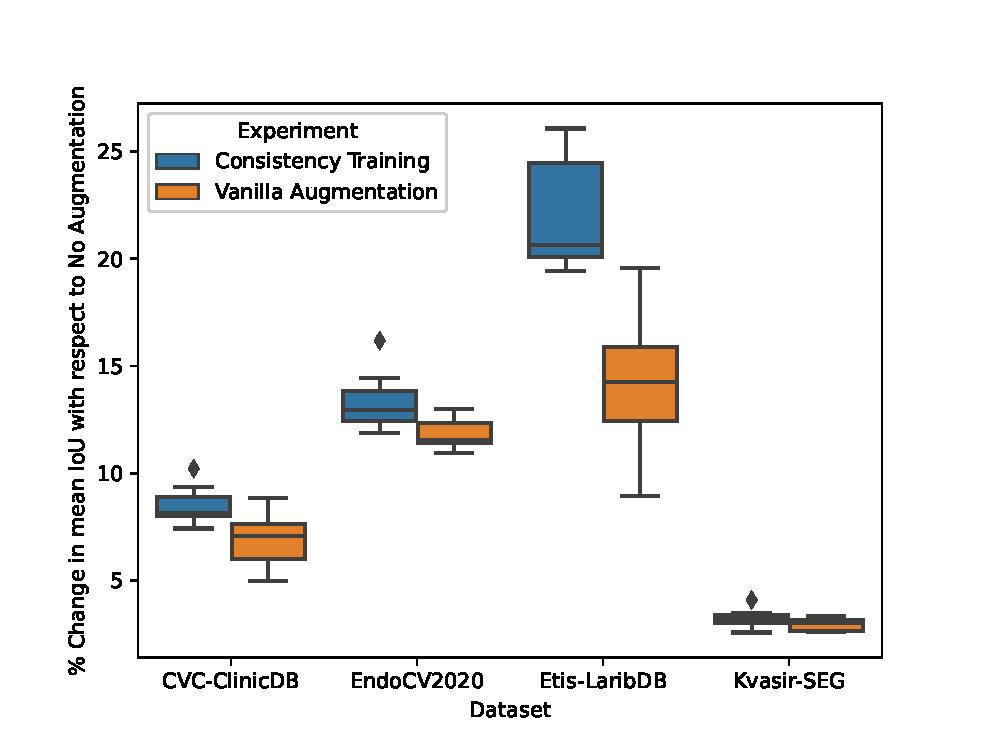
\includegraphics[width=\linewidth]{illustrations/consistency_training_percent.eps}
    \caption[Consistency Training improvements]{Improvements due Consistency Training and Data Augmentation as a percentage the mean \gls{iou} without augmentation across datasets}
    \label{fig:consistency_training_improvement}
\end{figure}

As discussed in~\Cref{cons_vs_aug}, this is to be expected. Though data augmentation and Consistency Training both increase the support of the models, only Consistency Training explicitly imposes inductive biases, and hence provides a better basis towards increasing generalization. This is also evidenced by considering the performance variability across the configurations,  shown in~\Cref{fig:consistency_cstd}.

\begin{figure}[htb]
    \centering
    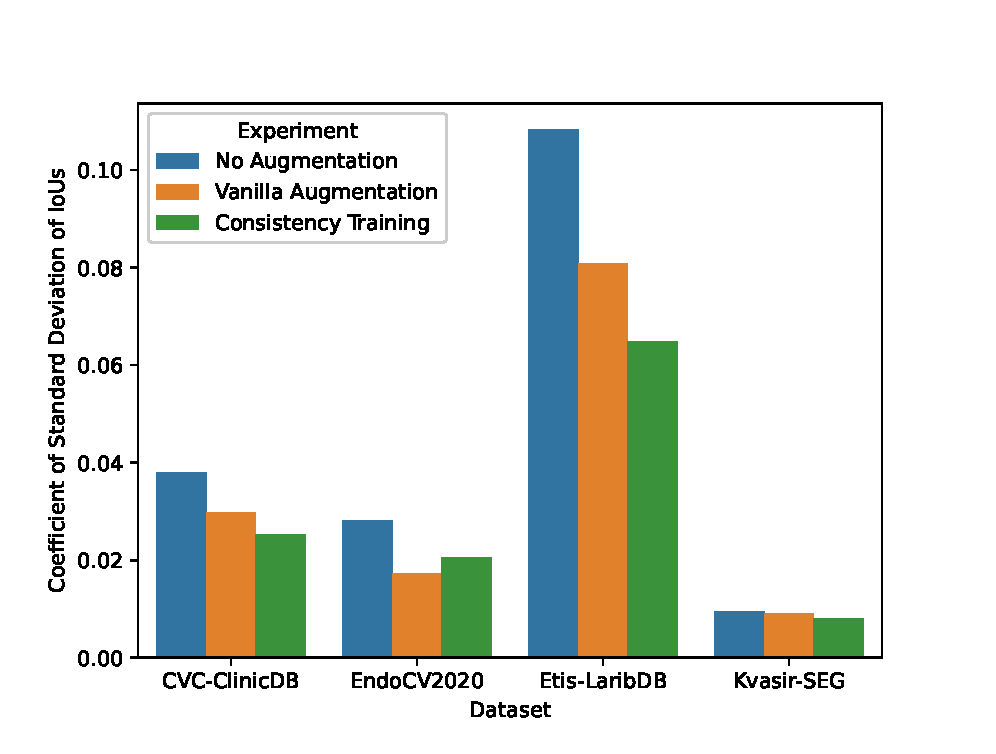
\includegraphics[width=\linewidth]{illustrations/consistency_training_cstd.eps}
    \caption[Consistency Training performance variability]{Models trained with Consistency Training exhibit lower predictor-wise performance variability than models trained without augmentation or with regular data augmentation}
    \label{fig:consistency_cstd}
\end{figure}

\section{Ensembles}\label{ensembles}

Finally, the impact of combining multiple predictors into an ensemble was investigated. Two types of ensembles were investigated: ensembles consisting of five instances of a single type of model and ensembles consisting of all five models. The generalizability of these ensembles were then compared to one another and with the average performance of their constituent predictors. For completeness, ensembles consisting of predictors trained with regular data augmentation were also tested.   

To ascertain the generalizability of the ensembles to statistical significance, ten ensembles of each kind were implemented. For the multi-model ensembles, each of the ten ensembles was built from unique predictors trained in~\Cref{consistency_training}.  For the single-model ensembles, five predictors were randomly selected from the ten that were trained in~\Cref{consistency_training}. As will be further discussed in~\Cref{discussion}, these ensembles too should have been built from unique predictors, however due to limits of computational resources this was not possible. 

\begin{table}[htb]
    \centering
    \begin{tabularx}{\linewidth}{lXXXr}
\toprule
Ensemble  & CVC-ClinicDB & EndoCV 2020 & Etis-LaribDB & Kvasir-Seg \\
\midrule
\multicolumn{5}{c}{Consistency-Trained}\\
\midrule
DD-DeepLabV3+   & 0.748 &0.684 &0.492 &0.863 \\
DeepLabV3+      & \textbf{0.751} & 0.683 & \textbf{0.523} &0.859 \\
FPN             & 0.739 & 0.685 &0.478 & 0.868 \\
Unet            & 0.744 & 0.694 &0.494 & 0.868 \\
TriUnet         & 0.723 & \textbf{0.715} & 0.468 & 0.859 \\
MultiModel      & 0.747 & 0.693 &0.484 &0.867 \\
\midrule
\multicolumn{5}{c}{Conventional Augmentation}\\
\midrule
DD-DeepLabV3+   & 0.749 & 0.684 & 0.495 & 0.865 \\
DeepLab         & 0.749 & 0.691 & 0.486 & 0.863 \\
FPN             & 0.732 & 0.686 & 0.454 & \textbf{0.871} \\
TriUnet         & 0.720 & 0.692 & 0.451 & 0.861 \\
Unet            & 0.734 & 0.675 & 0.437 & 0.869 \\
MultiModel      & 0.740 & 0.687 & 0.462 & 0.867 \\
\bottomrule
\end{tabularx}
    \caption[IoUs across ensemble models and datasets. ]{IoUs across ensemble models and datasets. Best ensembles for each dataset are highlighted in bold.}
    \label{tab:ensembles}
\end{table}

\begin{figure}[htb]
    \centering
    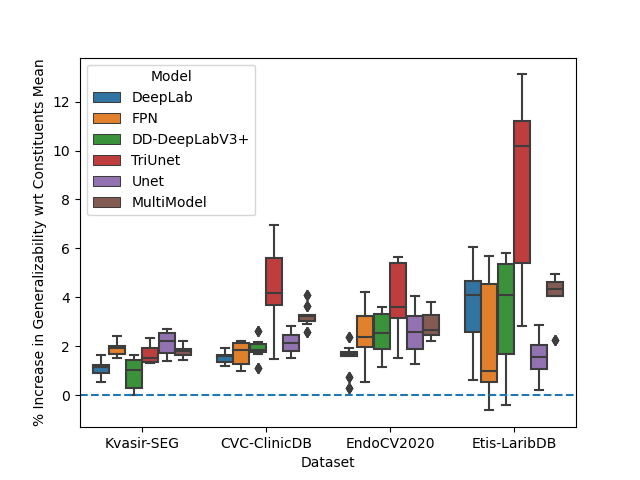
\includegraphics[width=\linewidth]{illustrations/improvements_due_to_ensembles.png}
    \caption[Improvements due to Ensembles]{Boxplot showing the improvement due to ensembles as a percentage of the mean \gls{iou} across their constituent models}
    \label{fig:ensemble_improvements}
\end{figure}
The \gls{iou}-scores for the ensemble models are shown in~\Cref{tab:ensembles}. The ensembles consisting of predictors trained with Consistency Training exhibited increased generalization on EndoCV2020 and Etis-LaribDB by a statistically significant margin (p<0.01). The differences between the two predictor training types was statistically insignificant for the CVC-ClinicDB dataset. Interestingly, the ensembles trained with standard augmentation exhibit higher \gls{ind} performance by a statistically significant margin (p<0.01), though it should be noted that the difference is negligible. All p-values can be found in~\Cref{tab:ttest_avgs_ensemble} in Appendix A. 

To analyze the impact of ensembles with respect to single models, one can consider the relative performance improvements between them. To this end, the performance of the ensembles trained with Consistency Training was compared to the mean performance of its constituent models. The relative improvements as a percentage of the constituent predictor performance is shown in~\Cref{fig:ensemble_improvements}. Holistically, the results show that ensembles increase generalization. 

This, as mentioned in~\Cref{background}, is often attributed to the fact that ensembles mitigate underspecification. Specifically, they constitute a form of Bayesian marginalization, and should thus in theory be able to leverage the variability of its constituent predictors in order to increase generalization.

To investigate the veracity of this line of reasoning, one can consider the relationship between the improvements to generalization due to the use of ensembles versus the degree of underspecification for the pipelines that generate the constituent models. This is shown in~\Cref{fig:ensemble_var}. 
\begin{figure}[htb]
    \centering
    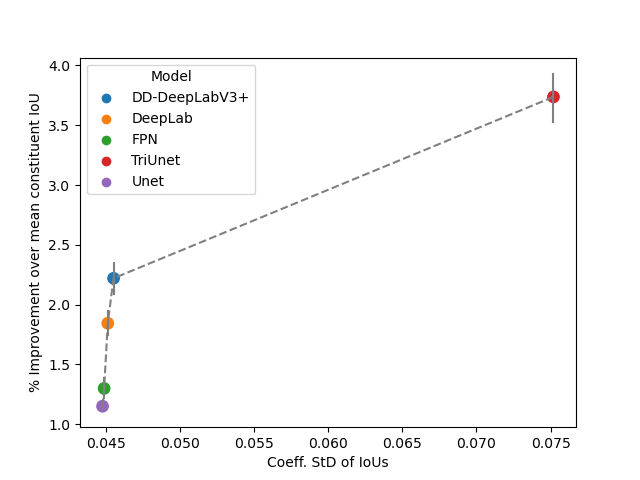
\includegraphics[width=0.75\linewidth]{illustrations/ensembles_underspecification.png}
    \caption[Relationship between ensemble improvements and underspecification]{Plot showing the relationship between predictor-wise performance variability and improvements in generalization due ensembles. The error-bars show the 95\% confidence intervals for the improvement. The more under specified the pipeline is as quantified by performance variability, the greater improvements are made through the use of ensembles}
    \label{fig:ensemble_var}
\end{figure}

There appears to be a positive relationship between the two, which corroborates the aforementioned interpretation. It should be noted, however, that the relatively low sample size and consequent potential errors in the estimate for the \gls{cs} means that this relationship cannot be determined with statistical certainty. This will be discussed further in~\Cref{discussion}. 

In~\Cref{fig:ensemble_var}, it should also be noted that the \gls{cs} values are computed based on all ten samples, as it is supposed to represent the degree to which the pipeline is underspecified, and not the variability of the constituent predictors for each ensemble instance. If one instead considers the variability in performance of the constituent predictors - which it can be argued is a better representation of the diversity of features learned by the ensembles. This is shown in~\Cref{fig:ensemble_var_stat}.

\begin{figure}[htb]
    \centering
    \hspace*{-1.9cm}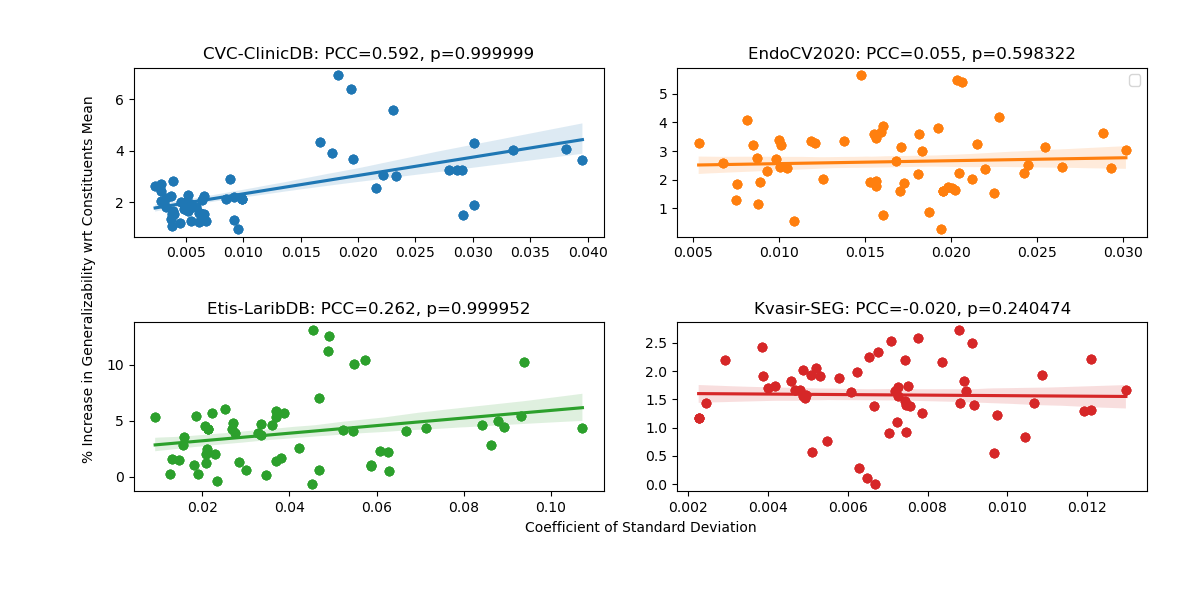
\includegraphics[width=1.2\linewidth]{illustrations/ensemble_variance_relationship_statistical.png}
     \caption[Relationship between ensemble improvements and constituents' performance variability]{Plot showing the correlation between the improvements to \gls{iou} with respect to the mean \gls{iou} of the constituent predictors, versus the variability in the performance of the constituent predictors. The Pearson Correlation Coefficient and corresponding p-value for each dataset is shown in the title of each subplot.}
    \label{fig:ensemble_var_stat}
\end{figure}

The \gls{cs} values are in this case based on five predictors - half as many as in~\Cref{fig:ensemble_improvements} - and there are consequently greater possible margins for measurement error. Nevertheless, there appears to be a positive relationship between predictor-wise performance variability and the performance improvements with respect to the mean performance of the constituents for two of the three \gls{ood} datasets. The relationships do, however, appear somewhat spurious, and the p-values shown above each subplot may be misleading, as the the relationships do not appear to be particularly linear. 

\section{Summary}
This chapter detailed the experiments performed to evaluate the methods presented in~\Cref{methods} along with the effects of model architecture, augmentation, and ensembles on generalizability. The results can be summarized as follows:
\begin{itemize}
    \item Model architecture had limited bearing on increasing generalization, but large models are likely to harm it.
    \item Multitask learning as implemented using the Dual-decoder DeepLabV3+ had negligible impact, which may be attributed to the encoder learning dataset-agnostic features.
    \item Data augmentation increased generalization considerably, but the use of the generative inpainter had a negative effect.
    \item Consistency training outperformed conventional data augmentation, and increased generalization by significant margins on more difficult datasets.
    \item Ensembles models increased generalization. The relationship between this increase and underspecification was investigated, and though there appeared to be a positive correlation, this was not conclusively proven.
\end{itemize}

These findings will be discussed in further detail in~\Cref{discussion}. 

    \chapter{Analysis and Discussion}\label{discussion}
This chapter will summarize the key findings presented in~\Cref{experiments} and analyze them with respect to the theory as outlined in~\Cref{background}. The chapter will be organized according to the experiments performed, with each section discussing the results, impact, and limitations of the corresponding experiment. The chapter will start with the results from the individual experiments, including the impact of model architectures on generalization as presented in~\Cref{models}, the impact of augmentation as presented in~\Cref{augmentations}, inconsistency Training as presented in~\Cref{consistency_training}, and finally ensembles as presented in~\Cref{ensembles}. Afterwards, the generalizability of the best performing configuration tested in this thesis will be discussed and considered from a practical perspective.


\section{Model Architectures and Generalizability}\label{discussion:models}
The experiments performed in~\Cref{models} show that every model exhibited comparable levels of generalisation failure, with the exception of TriUnet which seemed to struggle more than any of the other models. On Etis-LaribDB, which evidently proved to be the most difficult dataset, every model exhibited a generalizability gap of at least around 50\%, with the TriUnet ranging upwards of 65\%. The degree of generalization failure was slightly less pronounced on the two other datasets, with CVC-ClinicDB exhibiting average gaps of approximately 18\% and EndoCV2020 25\%. 

The models exhibited comparable performance also in \gls{ind} settings, spanning between IoUs of 0.819 and 0.832, which for practical purposes can be considered negligible. 

\subsection{Impact}
Naturally, deploying any of the predictors from this experiment in a clinical setting would be inadvisable and perhaps even harmful. Even if the predictors were to be trained on a dataset collected exclusively from the centre they were intended to be deployed on, there is no guarantee that there would never be some form of distributional shift, which as evidenced by the results significantly affect performance. This distributional shift may be as simple as a change in endoscopy preparation routines, or perhaps an upgrade to a higher resolution cameras, and so on. As established in~\Cref{background}, a system based on models with this lack of generalizability would be practically useless. 

Moreover, these results highlight that researching the development of more and more complicated task-agnostic models is a comparatively fruitless affair. The difference between DeepLabV3+ and Unet - which are separated by two years of research - are practically inconsequential. Admittedly, the differences are more pronounced when the models are trained according to the more sophisticated training regiments used in the remaining experiments, but it is nonetheless clear that it is not advancement in model architectures that is likely to result in increased generalization, but rather improvements to the pipeline with which they are trained.

\subsection{Limitations}\label{pretraining}
        A largely neglected but nevertheless impactful aspect of the deep learning pipelines studied in this thesis is the use of pretraining. Across all the experiments performed in this thesis, every predictor was pretrained on Imagenet, with the pretrained weights being included in the segmentation-models-pytorch library~\cite{smp}. Without pretraining, the models selected in this thesis exhibited \glspl{iou} of at best around 0.6 at best even on \gls{iid}, with even more significant performance gaps on \gls{ood} data. Naturally, non-pretrained networks are for this reason rarely used. However, this pretraining may play a key role in certain aspects of the behaviour observed in this thesis. In particular, pretraining may be the principle contributing factor behind the apparent ineffectiveness of multitask learning. An Imagenet pretrained encoder would, after all, perform the best when practically performing image compression.

\section{Data Augmentation and Generalizability}
The experiment in~\Cref{augmentations} demonstrated the efficacy of data augmentation as a means of increasing generalization, with an \gls{iou} improvement of 9.00\% compared to the pipeline without data augmentation when averaged across models and datasets. This, as mentioned in~\Cref{probpersp}, can be attributed to the fact that a wider diversity of data limits the space of viable features that a model can learn. 

\subsection{Impact}

What is surprising is the extent to which augmentation improves generalization in comparison to some of the other tested methods. In particular, the effects of model architectures and ensembles were both comparatively small. The use of ensembles, for instance, the use of which was the basis of several of the papers submitted to EndoCV2021, increased generalization by at most \(10.36\%\) and on average \(2.48\%\), whereas the use of data augmentation led to increases of at most \(19.57 \%\) and on average \(9.00\%\) when compared to no augmentation.

Thus, the margins by which the use of augmentation affects generalization are far greater than the margins by which ensembles and perhaps many of the other methods presented in EndoCV2021 affect generalization. This raises questions as to the validity of the results in EndoCV2021, which did not control for the choice of data augmentations when comparing submissions. It may, for instance, be the case that certain submissions exhibited high degrees of generalization not strictly because of the impact of their proposed methods, but rather due to their choice of augmentations. This is of course not a certainty, and does as such warrant further research for instance in the form of a meta-analysis. 

\subsection{Limitations} \label{augmentation_limitations}
    Ignoring the inpainter and its flaws as outlined above, only one implementation of data augmentation was used throughout this thesis. The constituent transformations and the values of the hyperparameters thereof were also selected with limited prototyping or testing. There may as such be augmentation configurations that induce significantly increased generalization. By the same token, the selection of transformations used in this thesis may instead have been lucky and thus over-represent the typical contribution of data augmentation. A robust investigation of data augmentation and its effects would require a larger range of augmentation strategies. The results thereof would, however, only be of relevance to the particular task that is being considered. Polyp segmentation may benefit more from augmentation than image-captioning, for instance. 
    
    Additionally, the augmentations in this thesis were applied according to a predetermined probability. A more effective technique may be to augment every sample, but account for the severity through the modulation of the hyperparameters of the constituent transformations. This was not, however, investigated in this thesis, as the probability-based implementation facilitated more apples-to-apples comparison to Consistency Training. 

\section{Consistency Training and Generalizability}
Consistency training was shown to improve generalizability, outperforming data augmentation by a significant margin on all \gls{ood} datasets. This can be attributed to the additional inductive that are imposed.  
        
    \subsection{Impact}
    Though Consistency Training did increase generalization by a considerable amount, the \gls{ood} performance is nevertheless insufficient for practical purposes. The best performance on Etis-LaribDB with Consistency Training was after all merely 0.504, as shown in~\Cref{tab:consistency}. This kind of performance would naturally be of limited utility in clinical applications.
    
    Consistency Training does, however, constitute a step in the right direction. In contrast to competing methods such as Model-Based Robust Deep Learning \cite{modelbased}, Invariant Risk Minimization \cite{IRM}, or multi-domain training \cite{generalization_datamod}, Consistency Training only requires a single dataset, and can as a result be used in practically every segmentation pipeline. The implementation thereof is also conceptually simple, and can for practical purposes be considered a more generalizable alternative to data augmentation. 
    
    Given further development, Consistency Training may prove a promising candidate as a means of alleviating generalization failure to practically viable extents, especially if leveraged in conjunction with other methods. As established in~\Cref{methods}, the limits are in theory only the efficacy of the quantification of consistency for a given task and the extent to which the augmentation strategy can account for any distributional shifts that may occur. Improvements to either of these aspects are likely to contribute to considerable gains in generalizability. 
    
    Developing perturbation models and consistency metrics may also be a great opportunity to incorporate expert input. A clinician could for instance offer insights as to the nature of the perturbations one might expect in practice and thus assist in the development of the perturbation model.
    
\subsection{Limitations}
    During the experiments performed in this thesis, the batch size was set to 8 for all training procedures. As Consistency Training relies on generating pairs of data from a given batch, one may argue that keeping the batch size the same may result in a weak comparison. The experiment should as such ideally be repeated across a number of batch sizes, but this was infeasible due to logistical constraints, in particular with regards to computational resources. 


\section{Ensembles and Generalizability}
    The use of ensembles, as shown in~\Cref{ensembles}, was proved to increase generalization. The improvements were on average comparatively minor, however increasing generalization by 2.026\%, 3.081\% and 2.351\% respectively for ensembles trained with no augmentation, conventional augmentation, and Consistency Training.  To reiterate, data augmentation contributed an average improvement of 9.00\% and Consistency Training 11.73\% over no augmentation. 
    
    Moreover, the differences in improvements between ensemble training methods was not found to be statistically significant. Thus, the findings in this thesis suggest that ensembles 
    
    
    
    Finally, the findings as presented in~\Cref{fig:ensemble_var} do to some extent support the hypothesis that this improvement is a consequence of the fact that ensembles mitigate underspecification, as the greatest gains to generalization were achieved by models that initially exhibited high degrees of underspecification as quantified by the performance variability of the respective pipelines. This was not, however, proven with statistical certainty, and requires higher sample sizes and ideally a larger diversity of model-architectures to verify to statistically significant extents.  

    
    \subsection{Impact}
    The use of ensembles was in this thesis proven to be a comparatively simple and reliable way of increasing generalization, albeit by a minor amount. It should also be noted that ensembles incur higher costs with regards to training time, time required for inference, and memory requirements. This, naturally, needs to be weighted against the benefits, which as discussed are fairly marginal on average. It may for instance be the case that the computational resources spent training multiple predictors for use in an ensemble would be better spent tuning the augmentation strategy if a \gls{ood} dataset is available. As the results in \Cref{augmentations} show, the choice of augmentation strategy appears to have a more significant impact on generalization than the use of ensembles. Thus, the findings in this thesis suggest that testing N different augmentation strategies may be a better use of resources than training N identical predictors to be used in an ensemble. Granted, this is difficult to say with certainty without exploring a larger diversity of augmentation strategies as discussed in \Cref{augmentation_limitations}.
    
    The analysis of ensembles in the context of underspecification performed in \Cref{ensemble_underspecification} showed that
    
    \subsection{Limitations}
    As mentioned in~\Cref{ensembles}, the constituent predictors for each ensemble were sampled from the ten predictors trained for the purpose of the experiments in~\Cref{augmentations} and~\Cref{consistency_training}. As a result, the statistical significance of the findings are not necessarily robust. Thus, the experiments should ideally be repeated with an increased sample size, for instance N=50, such that ten ensembles could be constructed such that each ensemble consists of an independent set of predictors. 
    
    It should also be noted that the experiments in this thesis were performed only at one ensemble size - i.e, five models. This choice was informed by the literature, in particular the implementation of DivergentNet \cite{divergentnets}. Ensembles may as such have a greater impact than expected, dependent on the returns from increasing the model counts. Following the Bayesian perspective as discussed in~\Cref{background:ensembles}, increasing the model count may result in a better estimate of the Bayesian posterior, and thus lead to increased generalization.
    
    The improvements from increasing ensemble size may however be limited. The performance of ensembles is after all bounded by the performance of perfect Bayesian marginalization. As shown in~\Cref{fig:bayesian_generalization}, this will not necessarily constitute perfect generalization, as the predictions are in such a system weighted according to the likelihood that the given weight configuration is returned from the pipeline. Thus, if learning shortcuts is likely, Bayesian marginalization will primarily be predicting according to shortcut features. Investigating this may be an interesting direction of further study.
    
    Finally, the method by which ensembles were implemented in this thesis - in particular, that the heatmap is thresholded with majority vote - may under-represent the potential utility of ensembles. By requiring that at least half of the constituent predictors are in consensus in order to consider a given pixel as a positive prediction, some potentially insightful predictions may be discarded. A better alternative is to consider the heatmap as a whole, which in any case would be more informative in a clinical setting. Evaluation of ensemble models should thus ideally take this into account. 


\section{Overall Impact}
Though this thesis presents methods that constitute considerable improvements to generalization, the best performing system - namely the DeepLabV3+ ensemble trained with Consistency Training -  would nevertheless not be particularly useful in practical settings when considered holistically.

This system achieved average \glspl{iou} of 0.751 on CVC-ClinicDB, 0.683 on EndoCV2020, 0.523 on Etis-LaribDB, and 0.859 on Kvasir-SEG. Though this constitutes a considerable improvement over both of the "naive" pipelines - i.e single models trained with and without regular data augmentation - it is nonetheless not sufficiently generalizable for practical use. Ideally, there should be negligible differences between all four datasets, and though there is room for some degree of performance degradation, a system that exhibits a mean \gls{iou} of 0.523 is not particularly useful and as discussed in~\Cref{ethics} may actually cause more harm than good. 

Thus, in spite of the aforementioned improvements, the pipeline as a whole is not in purely practical terms much better than any of the naive pipelines. More work is evidently required to achieve suitable levels of generalization. Some ideas for directions of further work towards this end will be discussed in \Cref{conclusion}. 
\section{Limitations of the Experimental Methodology}

\subsection{Metrics selection}

\cite{metric_weakness}
As this thesis focused on the differences in performance between \gls{ood} and \gls{ind} datasets, the only metrics that were considered was the \gls{iou} and the \gls{cs} of the \gls{iou}. Though \gls{iou} is a very popular metric for evaluating segmentation pipelines and is easy to interpret, it is not without its flaws~\cite{metric_weakness}. It is for instance typically biased against small structures, as these are affected to a greater degree by errors that in practical terms are comparatively minor. This can result in misleading mean \glspl{iou}, in particular when the distribution of object sizes is wide, as is indeed often is the case with polyps datasets~\cite{endocv2021_review}.  

Ideally, more metrics should have been considered, for instance precision, recall, and perhaps even \gls{sis}, in order to paint a more complete picture of the performance of the tested methods. 

\subsection{Dataset Selection}
This thesis considered three \gls{ood} datasets throughout all the experiments. Though this provides some indication of generalizability, ideally even more \gls{ood} datasets should have been used. For instance, though Etis-LaribDB was the most difficult of the datasets used in this thesis, the performance on this dataset does not necessarily reflect the worst-case performance in a clinical setting. Indeed, the extent to which the a given pipeline fails to generalize cannot be sufficiently anticipated \cite{trust_ai} given current approaches to deep learning. It may easily be the case that the model performs even worse under certain clinical conditions. Without a larger sample of \gls{ood} datasets, there is a high degree of uncertainty involved as to the actual ability of the given systems to generalize. Though the low generalizability of the systems implemented in this thesis means that this has little practical bearing, any future research that reports generalizability of practical merit should concentrate a significant effort on assembling a large collection of \gls{ood} datasets. 

As briefly mentioned in \Cref{datasets}, the methods presented in this thesis should ideally have been compared to the works presented in EndoCV2021~\cite{endocv2021}. As the datasets used to evaluate the submissions was not available at the time of writing this thesis, however, this was infeasible. 

\subsection{Model Architectures}
To validate that the impact of the proposed methods translated across models, and to determine the impact of model architectures, this thesis implemented five separate models - i.e DeepLabV3+, DD-DeepLabV3+, FPN, Unet, and TriUNet. 

It can be argued that these models do not capture the diversity of segmentation models available, however.

\section{Summary}
This section presented a more thorough analysis and discussion of the findings as presented in~\Cref{experiments}. The results were analyzed with respect to the literature, the theory as laid out in~\Cref{background}, and considered in terms of viability of clinical deployment. For each experiment, the impact, limitations and potential improvements were discussed where applicable. 

Holistically, the findings in this thesis highlight that generalization remains a challenging problem, but that the development of generalizable methods is an endeavor ripe for further exploration. Consistency Training in particular seems to be a promising candidate for further research towards alleviating generalization failure. It was also shown that further foundational work is required in order to fully understand the relationship between the constituent components of the deep learning pipeline and generalizability, in particular with regards to developing sufficiently well-controlled experimental methodologies and eliminating confounding variables during comparative studies. 
    \chapter{Conclusion}\label{conclusion}
 
\section{Summary}
The goal of this work has been to develop novel methods of increasing the generalizability of deep learning models, as well as to survey the relative impacts of more conventional components of the deep learning pipeline. This was achieved as follows:

\Cref{background} provided an overview of deep learning, segmentation, and delved further into why such systems so readily fail to generalize, starting from first principles and analyzing the shortcomings of \gls{erm}. This was then connected to recent analyses of generalizability failure, including the notion of underspecification and shortcut learning. Finally, known methods of increasing generalization as presented in EndoCV2021 and elsewhere in the literature were then discussed and analyzed with respect to the established theory. 

This was then in turn used to inform the development of the methods discussed in~\Cref{methods}, including a novel training paradigm, augmentation technique, model architecture and ensemble models. Each of these methods were also discussed with respect to the theory explored in~\Cref{background}.

Several experiments were then conducted in~\Cref{experiments} in order to ascertain the impact of the proposed methods:
First, baseline generalizability metric were collected for five separate models. The findings supported the notion that larger models are more prone to generalizability failure, as demonstrated by the significant gap between the Unet and the TriUnet. The use of a secondary decoder in the DD-DeepLabV3+ model was shown to have negligible impact, despite reducing performance variability. It was hypothesized that this is due to the encoder already learning domain- and dataset-independent features. 

In the next experiment, data augmentation was shown to increase generalizability by a considerable margin. Synthetic augmentation via inpainting was shown to hamper this improvement when used in conjunction with regular augmentation, but this finding was deemed inconclusive due to the relatively low performance of the inpainter. 
The impact of Consistency Training was then tested and compared to regular data augmentation and no augmentation. The results show that Consistency Training outperforms regular data augmentation by a considerable margin on the most difficult of the three \gls{ood} datasets. 

Finally, predictors trained according to the best methods as identified in the previous experiments were then combined into ensembles. The results demonstrated the generalizability of ensemble-based methods, but further analysis did not sufficiently corroborate that this improvement can be attributed to ensembles mitigating underspecification. 

The results from this experiment was then discussed in~\Cref{discussion}. Limitations of the experiments were noted, along with their practical impacts and possible directions of further study and potential ways to improve the methods proposed in this thesis. 


\section{Contributions}
The contributions of this can be summarized according to the research objectives laid out in \Cref{introduction}:

\textbf{Objective 1}: \textit{To leverage recent advances in the understanding of generalization failure to inform the development of novel methods of increasing the generalization of deep learning systems for polyp-segmentation.}

This objective was achieved as through the introduction of several novel methods, the most effective of which being Consistency Training. By reframing the problem of generalization as consistency across perturbations, Consistency Training was shown to increase generalizability by a considerable margin without the need for multiple training domains, in effect serving as a more generalizable alternative to data augmentation. This framework, and the potential improvements that can be made upon it as suggested in~\Cref{discussion}, shows good promise with regards to further increasing generalizability. The ensemble models consisting of predictors according to Consistency Training was also shown to increase generalization, outperforming conventionally trained ensembles. Though the remaining methods - i.e generative inpainting and DD-DeepLabV3+ - were proven to be ineffective, the analysis thereof nevertheless motivated a number of directions of further study. 

\textbf{Objective 2:} \textit{To synthesize recent work on generalizability and determine concretely the degree to which more conventional and well-established methods affect generalization.} 

This objective was achieved by performing a quantitative analysis of the effect of the choice of model architecture, the use of data augmentation, and the use of ensembles on generalization. Though most of the findings corroborated the literature, there were a fair number of surprising results that warrant further investigation, in particular with regards to the impacts of the tested methods relative to one another. For one, the effect of multitask learning and generally the the choice of model architecture was in this thesis shown to be practically negligible. With the exception of TriUnet, every tested model exhibited practically identical performance. The use of ensemble-based model, though exhibiting statistically significant impact, resulted in somewhat marginal improvements on generalization, especially in comparison to the use of data augmentation and Consistency Training. As discussed in~\Cref{discussion}, this raises doubts as to the veracity of findings in other literature, where data augmentation is rarely accounted for when performing comparisons. Hopefully, the findings in this thesis demonstrate the need for a more structured approach to the design of experimental methodologies intended to analyze generalization, wherein the constituent components of the pipeline are sufficiently well controlled. 


\section{Future work} \label{future_work}
  There are several directions of future research that may provide further insight into generalizability and generalization failure. This section will cover a number of these ideas. 
  \subsection{Improving Consistency Training} \label{new_closs}
    As was shown in~\Cref{experiments}, Consistency Training is an effective means of increasing generalization. However, there is still room for further improvement and exploration. For instance, in this thesis consistency was expressed merely as the symmetric difference between the expected change in the output due to augmentation and the actual change due to augmentation. This, however, as discussed in~\Cref{methods}, is largely agnostic to the augmentation being performed. However, the nature of these augmentations should be taken into account. If the image is subjected to a 90 degree rotation, for instance, the prediction would be considered perfectly consistent so long as the pixels corresponding to the polyps are rotated, and the incorrectly classified pixels remain unchanged. However, if the model instead learns to rotate all of the pixels - even those that are incorrectly classified - it may learn a more accurate representation of what constitutes consistent behavior. I.e, instead of expressing inconsistency as:
\begin{equation*}
\mathcal{C}(a, \hat{a},y, \hat{y}) = \frac{\sum\{y \cap a \cap \hat{y} \cap \hat{a} \}}
{\sum\{ y \cup a \cup \hat{y} \cup \hat{a} \}}
\end{equation*}
    One can adjust the expected change term \(a\oplus y\) to \(\hat{y}\oplus \epsilon(\hat{y})\) such that also incorrect predictions can be considered consistent so long as they change in accordance to the nature of the perturbation model \(\epsilon(\cdot)\). The resulting loss function can then be expressed as:
\begin{equation*}
    \bar{\mathcal{C}}(y,a,\hat{y}, \hat{a}) = \sum \frac{\Theta(\hat{y}, \hat{a},  \hat{y}, \epsilon( \hat{y}))}{\bigcup(\hat{y}, \hat{a}, \epsilon(\hat{y}))}
\end{equation*}
Which is equivalent to:
\begin{equation*}
    \bar{\mathcal{C}}(\hat{y}, \hat{a}) = \sum \frac{\Theta(\hat{y}, \hat{a}, \epsilon( \hat{y}))}{\bigcup(\hat{y}, \hat{a}, \epsilon( \hat{y}))}
\end{equation*}
    This also has the advantage of being independent of the labels themselves. This may alleviate complications that may arise as a consequence of poor and/or incomplete labeling which would otherwise affect what the models learn to associate with consistent behaviour. 

    In addition to improving the way by which consistency is quantified, there are several unexplored directions through which the training procedure itself could be further improved. The perturbation model, for instance, could be modified in any number of ways: one could for instance adversarially sample difficult augmentations based on the consistency score, and use these during training. One could also perform a study to ascertain the impact of the perturbation models' constituent augmentation functions on generalization. It may for instance be the case that some of the augmentations used in the perturbation model used in this thesis hampered generalizability more than it facilitated it, though without a complete study this is impossible to say with any certainty.  
    
    One could also experiment with modulating the difficulty of the augmentations. In the experiments performed in this thesis, the augmentation difficulty was kept constant - i.e, the augmentation hyperparameters were capped to a specific range. However, it may be the case that gradually increasing the difficulty or modulate it according to some sort of annealing function could further improve the efficacy of Consistency Training. 
    
    Finally, using multiple perturbed images when computing inconsistency instead of just one may potentially further strengthen the generalizability of the learned features. In this thesis, the inconsistency term really only pertains to the inconsistency of the model with respect to the change being applied to the perturbed input. It is possible to  instead generate multiple perturbed inputs, each being transformed in a different manner, and then compute multiple inconsistency terms thereafter. This does require more memory, however, and may on certain hardware be infeasible unless the batch sizes are kept small. 
    
    \subsection{Deep Preprocessing} \label{denoising}
        In Consistency Training, the objective is to optimize for features that are consistent across perturbations such that the model learns invariance to distributional shifts that should not affect the causal structure of the problem. Though this as established increases generalizability, it may also be possible to simply preprocess the images such that \gls{ood} transformations or artifacts are accounted for. This is achieved elsewhere in the literature using generative models - for instance a CycleGAN~\cite{cyclegan}, which maps the input data between domains prior to being given to the segmentation network. One could implement a similar system using Consistency Training through the use of a denoising network. The resulting pipeline is illustrated in~\Cref{fig:preproc}.
        
        \begin{figure}[htb]
            \centering
           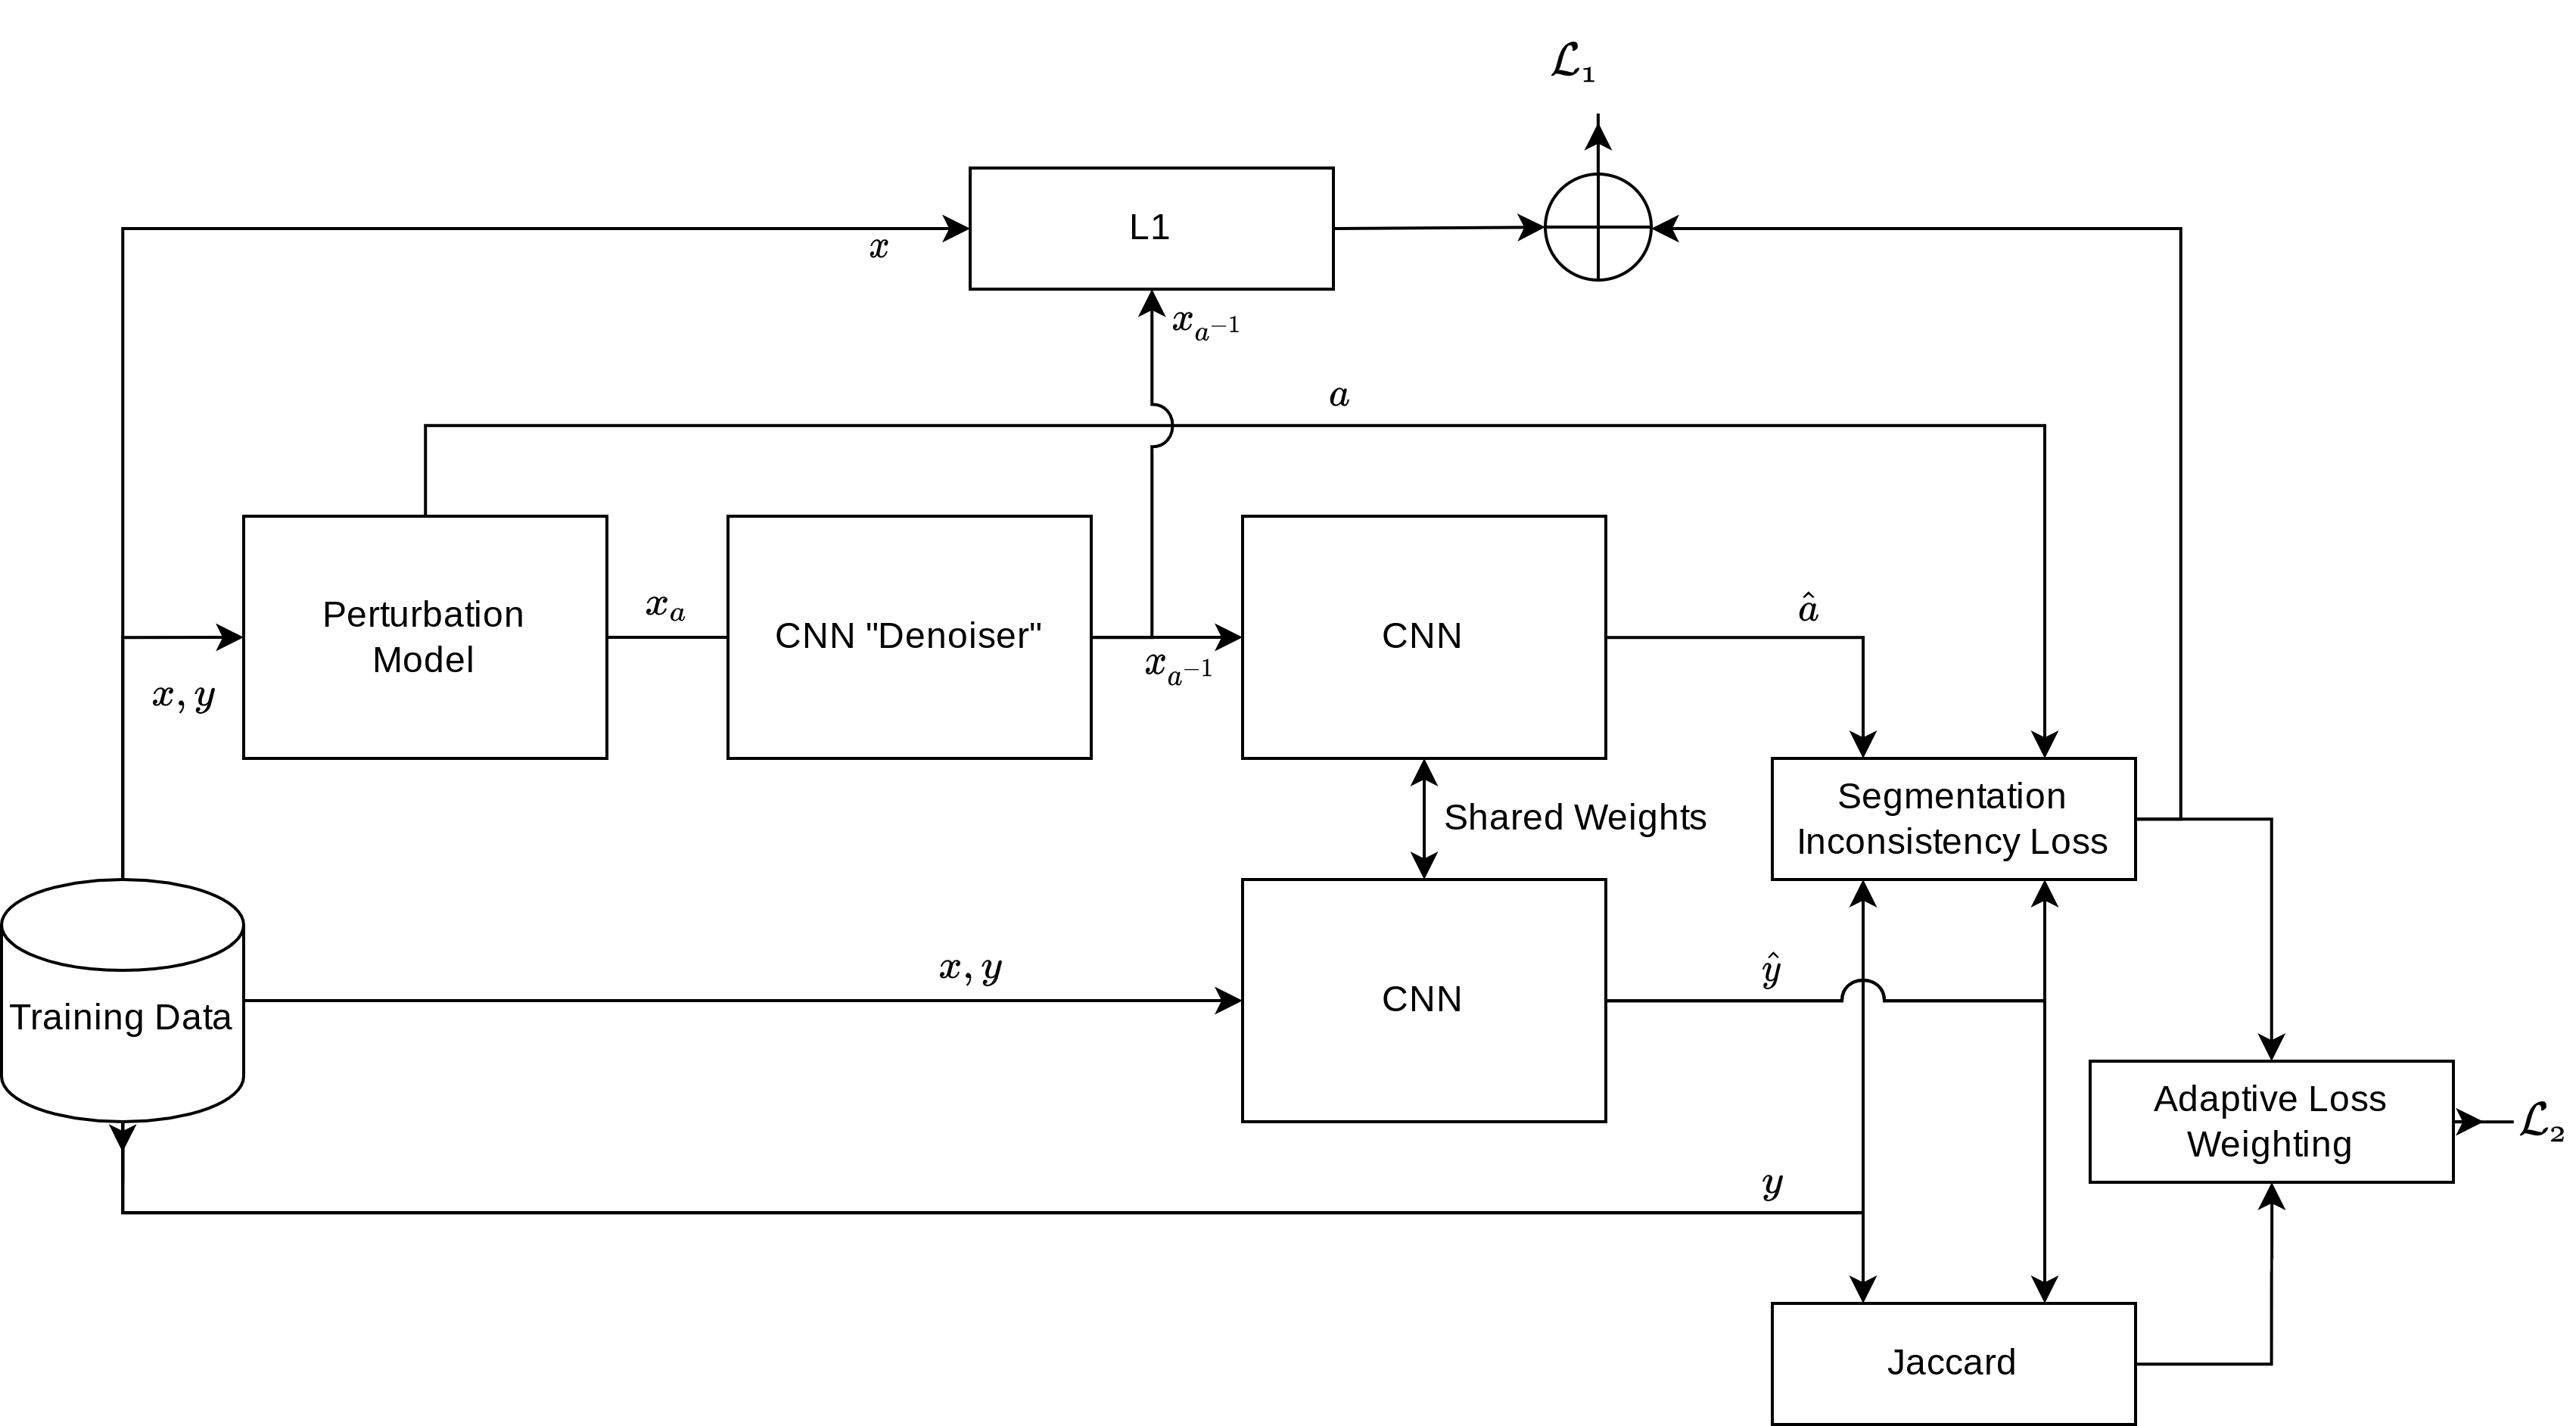
\includegraphics[width=\linewidth]{illustrations/deep_preprocessing.png}
            \caption{Consistency Preprocessing Pipeline}
            \label{fig:preproc}
        \end{figure}
        
        There are two main differences between this pipelines and more conventional deep denoising pipelines. First, the segmentation models are trained using Consistency Training. Second, the denoising network is incorporating inconsistency loss as a component of the loss function. There would in this case be two separate loss functions, one for each network. In theory, this should result in the denoiser learning to counteract the characteristics of the perturbations being applied that most negatively affect the consistency and thus the generalization of the segmentation models. Moreover, even if the denoiser performs poorly, the segmentation portion should be generalizable due to Consistency Training, which may even be improved as a result of whatever transforms the denoising network is performing.
        
    \subsection{Dual Decoder Models}
        \Cref{methods} introduced the dual-decoder DeepLabV3+, the intent of which was to increase generalization by constraining the space of latent representations that the model could leverage, thus in theory mitigating underspecification. As the results in~\Cref{dd-deeplab} showed, however, the effect of this additional encoder was fairly limited when compared to the regular DeepLabV3+. Though it was argued that the reduced performance variability of the dual-decoder model could be interpreted as evidence for a reduction in underspecification, the performance in terms of mean IoU was identical across both models for practical purposes. It was hypothesized that this may be due to the encoder learning principally dataset-agnostic features and consequently primarily performing image compression regardless of what object the model is intended to segment. 
        


        This was to some extent was corroborated by the analysis performed in~\Cref{dd-deeplab}, which showed equivalent image reconstruction performance across datasets in terms of L1 distance. Further research is however required, as these findings are only representative of one specific model trained in a limited number configurations. One possible direction is to implement a wide range of encoder-decoder models trained across multiple decoder tasks and datasets, and then investigate the latent spaces of the resulting predictors. If the predictor encoders indeed do encode primarily dataset-agnostic features independent of the decoder function, one would expect that one could simply switch encoders between predictors trained on different datasets, domains and tasks without significant performance degradation, at least after a few epochs of fine-tuning if for some reason the encoders have learned functionally different but practically comparable compression methods. 

        As discussed in \Cref{pretraining}, this behaviour might also be attributed to pretraining. Since the models used throughout this thesis were at least partially pretrained on Imagenet, it might simply be the case that the encoders have learned to perform image compression as a direct consequence of the fact that this likely is the most conducive configuration to minimizing risk on the Imagenet dataset. In this case, the encoder may be in such a wide minimum that actually learning domain-specific features is unlikely even after training to segment polyps. 

    \subsection{Further investigations of multitask learning}
        Multitask learning was only briefly investigated in this thesis through the dual-decoder DeepLabV3+, which as a reminder performed image reconstruction as an auxiliary tasks. Though this was shown to have negligible effects, which was hypothesized may be the result of segmentation encoders learning task-agnostic features - the results are by no means sufficiently conclusive to discredit multitask learning altogether. 
    
        Further investigating the impact of multitask learning on generalization is as such warranted. One could for instance perform a study on the impact of different tasks; perhaps image reconstruction is less conducive to generalization than something more task-adjacent, such as dimming the background or simple object detection. Depending on the results of this study, one could then also experiment with adding multiple auxiliary tasks. Investigating the variance of the latent representation in these models across multiple runs of training and comparing these to the variance in single-task models may be interesting and further the understanding of what \glspl{dnn} actually learn.
        
        Modifying the models to a greater extent than merely adding additional decoders would in this case also be warranted. One may for instance investigate whether the segmentation task could be decoupled into a series of multiple stages consisting of simpler tasks.
    
  
\subsection{Further Investigations on Inpainting and Generative Modelling}
The experiments in~\Cref{augmentations} showed that the use of an inpainter as implemented in this thesis harmed generalization when used in conjunction with conventional augmentations. Two hypotheses for why this is the case were suggested - either the inpainter simply does not perform to a sufficient standard conducive for use as augmentation, or the inpainter learned the distribution to such an extent that it increased the models' dataset bias. 

To investigate this, it is possible to implement one of the more state-of-the-art inpainting architectures, for instance an inpainting generative multi-column network \cite{inpainter_better}. Additionally, analyzing the generated polyps via statistical means may also have some merit. The development of distance metrics to facilitate easier comparison between synthetic images to real images may for instance be worth looking into, as this might shed some light on the hypotheses as presented above.

    \subsection{Improving Ensembles through Diversity Search}
    Though ensembles as implemented in this thesis exhibit somewhat limited returns, leveraging a diversity of interpretations of the input data may have considerable merit towards increasing generalization and clinical utility. As the analysis in~\Cref{fig:ensemble_var} shows, there appears to be a positive relationship between generalizability and model-diversity that warrants further investigation. In particular, it may be the case that ensembles consisting of predictors that are trained to explicitly encode differing features are more conducive to generalization than conventionally implemented ensembles. By explicitly optimizing for weight diversity, one might mitigate the tendency of typical ensembles to primarily consider weight configurations that exhibit higher posterior likelihoods. 
    
    This could for instance be achieved by training multiple instances of the same model concurrently, and incorporating some measure of the diversity of the learned feature maps across models into the loss function. A naive approach to this end could be to simply calculate the variance of each activation across every predictor. This is computationally expensive, however. A better approach is to select a subset of activations  - such as encoder outputs - and calculate the standard deviation across the predictors just for this subset.  An illustration of such a pipeline is provided in~\Cref{fig:diversity}.
    
    \begin{figure}[htb]
        \centering
        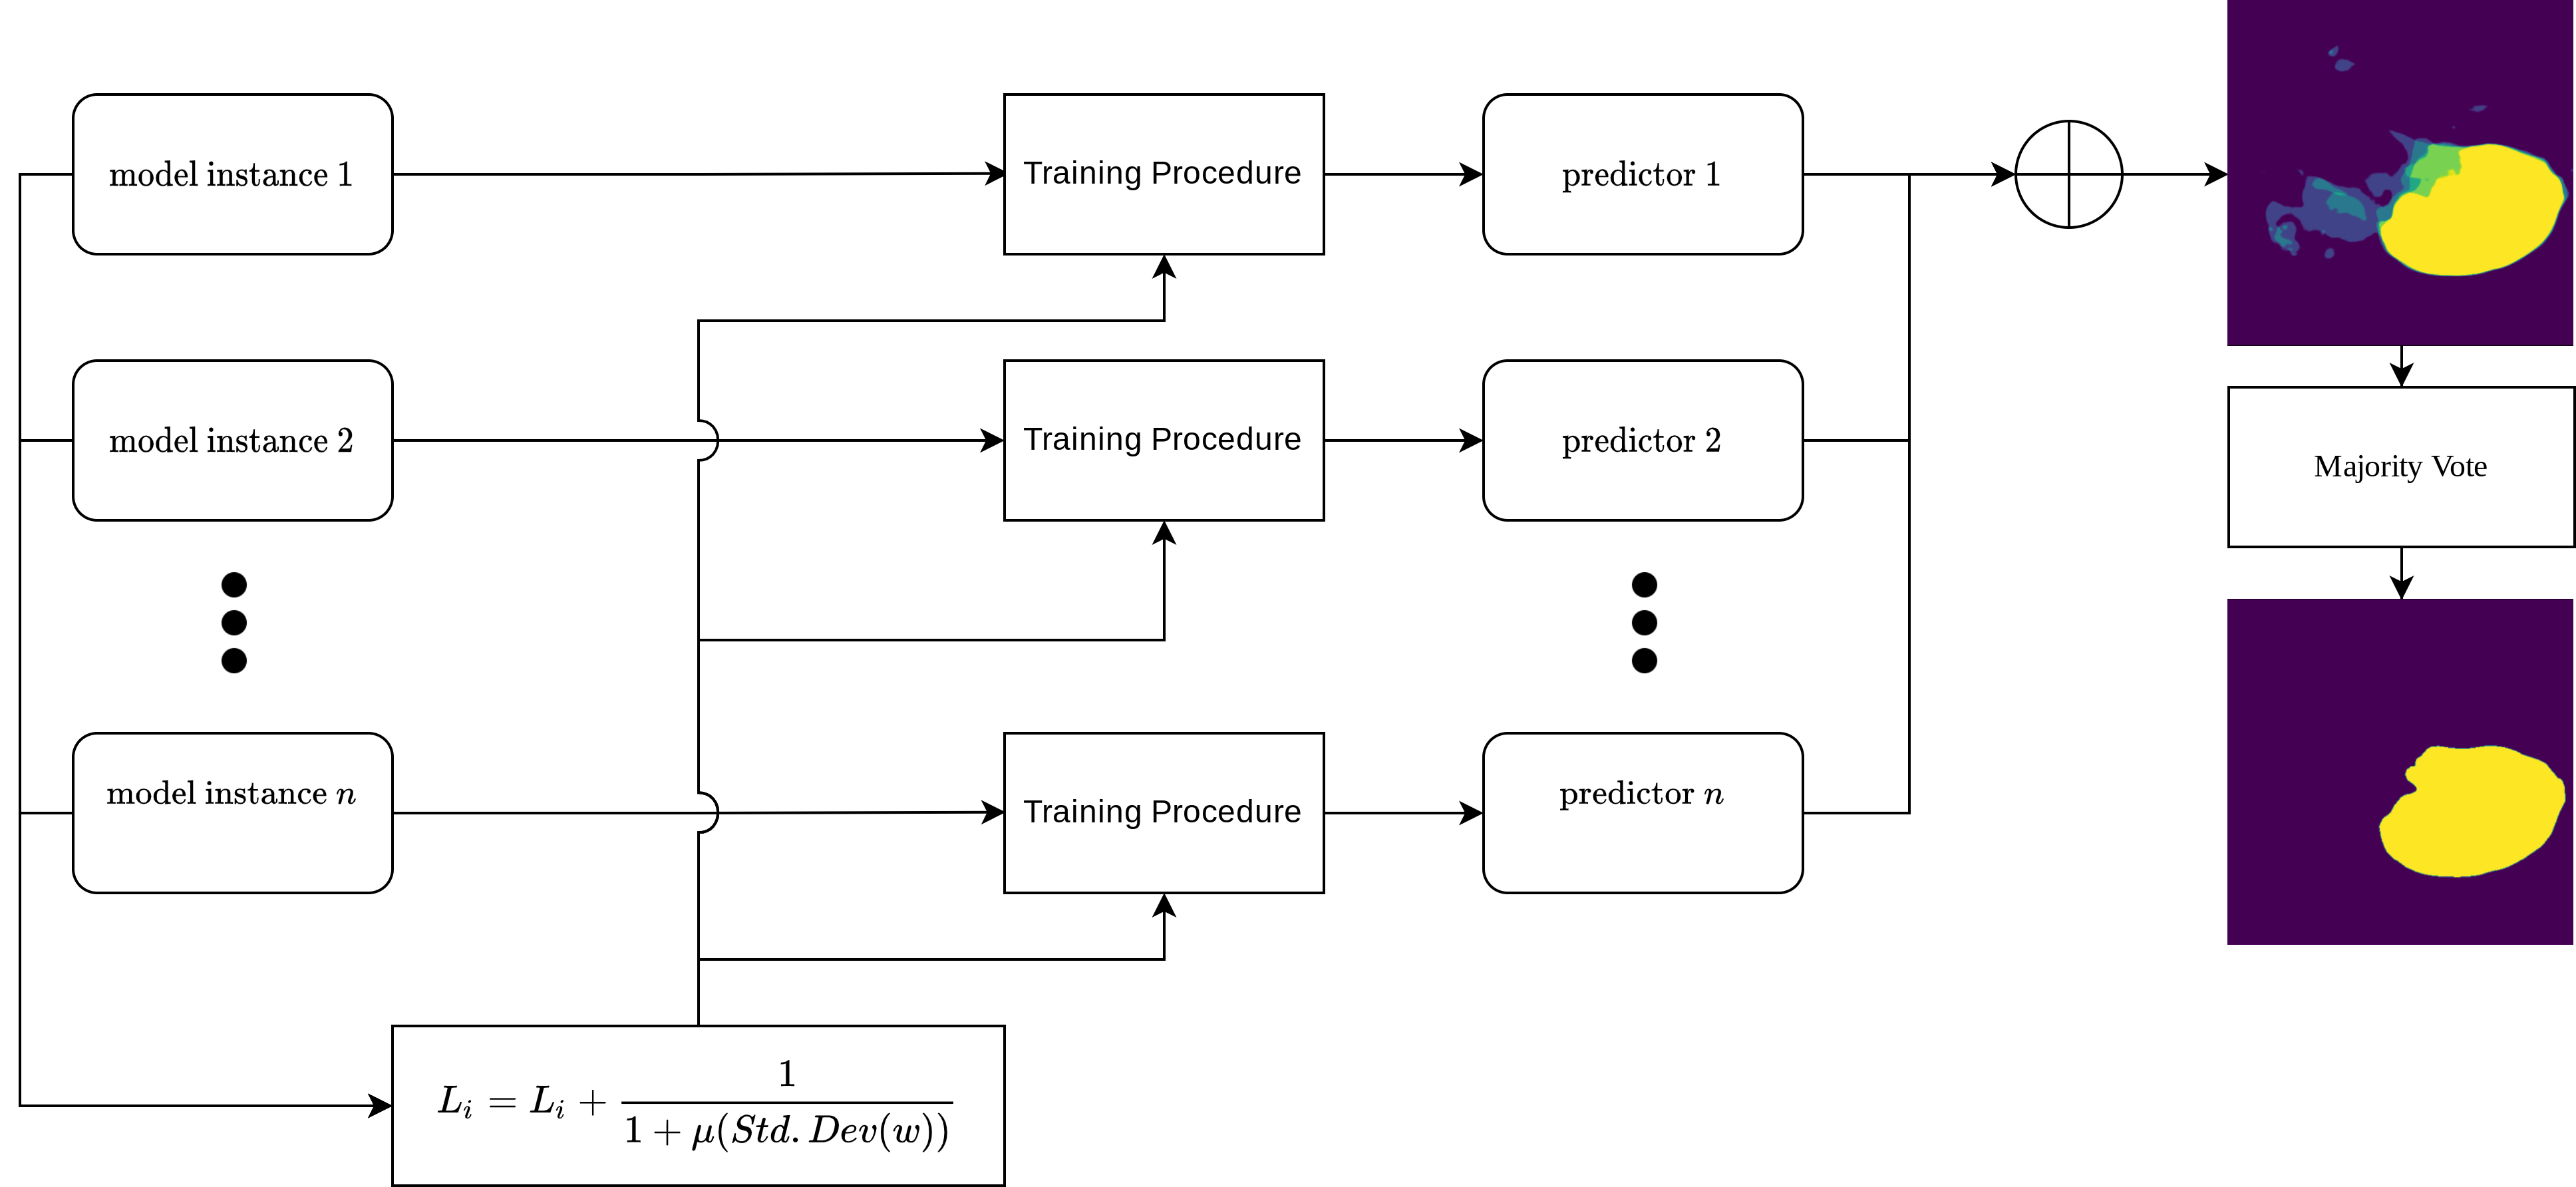
\includegraphics[width=\linewidth]{illustrations/diversity_search.png}
        \caption[Deep Diversity Search]{By adding a term corresponding to the mean standard deviation of weights, the models will learn maximally independent representations, and hence result in predictors with a larger diversity of learned features. This may mitigate underspecification to a greater extent, since this search would be less biased towards regions of the search landscape with high posterior probability.}
        \label{fig:diversity}
    \end{figure}
    
    This way, the ensemble will consist of predictors that encode a wider diversity of interpretations of the data than the predictors in conventional ensembles. This in turn provides a more complete perspective of the many possible interpretations a given model can learn. If this is proven to be the case, using the heatmaps from such an ensemble during screening may also actually be viable, as the clinician could then take all of these possible interpretations into account instead of trusting that a single predictor is encoding the right inductive biases.  

    \backmatter{}
    \printbibliography
    \chapter*{Appendix A: Code Access} \label{code_data}
\addcontentsline{toc}{chapter}{Appendix A}
All relevant code and data can be found on the GitHub repository: https://github.com/BirkTorpmannHagen/Master

\chapter*{Appendix B: p-values}\label{p-values}
\addcontentsline{toc}{chapter}{Appendix B: p-values}

\begin{figure}[hbt]
    \centering
    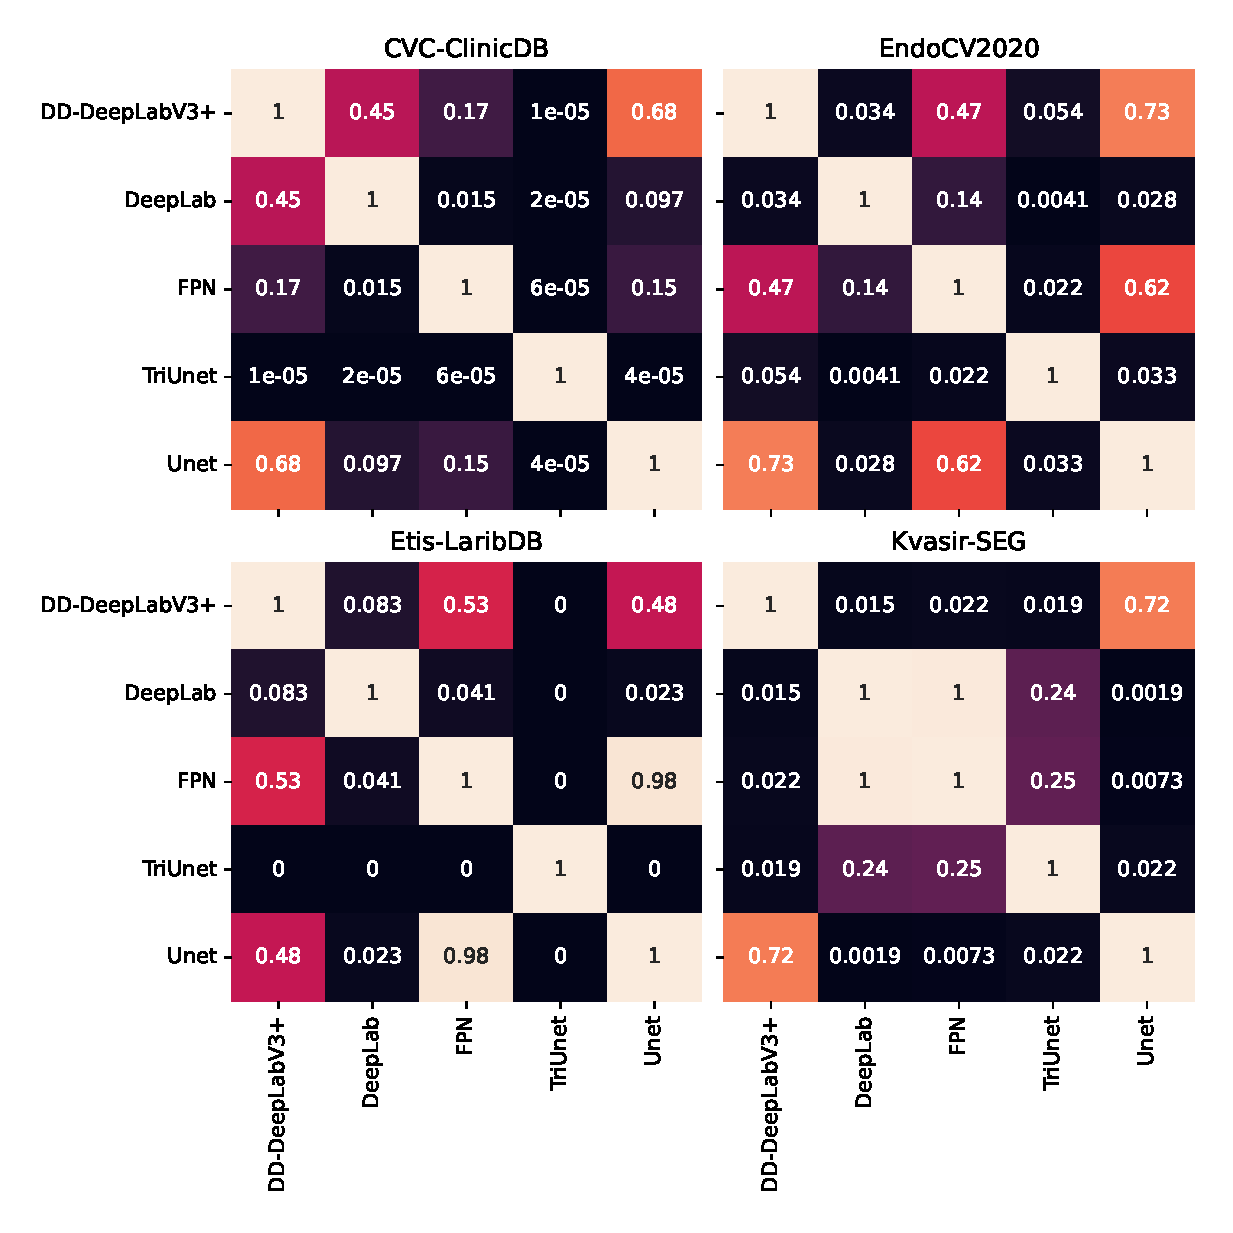
\includegraphics[width=\linewidth]{illustrations/model_pvals.eps}
    \caption{Two-sided independent t-test p-values between models for all datasets}
    \label{models_pvalues}
\end{figure}
% inpainter
\begin{table}[htb]
    \centering
    \begin{tabularx}{\linewidth}{lXXXX}
    \toprule
     Model & CVC-ClinicDB & EndoCV2020 & Etis-LaribDB & Kvasir-SEG\\
    \midrule
    DD-DeepLabV3+ & 0.04454 & 0.95857 & 0.12809 & 0.30201\\ 
    DeepLab & \textbf{0.0096} & 0.08898 & 0.11401 & 0.31065\\ 
    FPN & 0.13769 & 0.95284 & 0.17806 & 0.16613\\ 
    TriUnet & 0.13412 & 0.31111 & 0.19913 & 0.91489\\ 
    Unet & 0.01069 & 0.15406 & 0.02715 & 0.36489\\ 
      \bottomrule
    \end{tabularx}
    \caption[T-test results inpainting]{p-values for each model and dataset between the IoUs of the given models trained with  versus when trained with conventional data augmentation versus models trained with the inpainter as a component of the data augmentation strategy}
    \label{tab:ttest_per_dataset_inpainter}
\end{table}
\begin{table}[htb]
    \centering
    \begin{tabularx}{\linewidth}{lXr}
        \toprule
        Dataset & U-Statistic & p-Value \\
        \midrule
            Kvasir-SEG & 763.0, p=0.15972 \\ 
            Etis-LaribDB & 545.0, p=0.00163 \\ 
            EndoCV2020 & 851.0, p=0.4169 \\ 
            CVC-ClinicDB & 520.0, p=0.00077 \\ 
        \bottomrule
    \end{tabularx}
    \caption[Mann-Whitney U-test results inpainter averaged across models]{Results from Mann-Whitney U-test for each dataset when comparing the average \glspl{iou} of all models trained with conventional data augmentation versus models trained with the inpainter as a component of the data augmentation strategy}
    \label{tab:ttest_avgs_inpainter}
\end{table}

% consistency training
\begin{table}[htb]
    \centering
    \begin{tabularx}{\linewidth}{lXXXX}
    \toprule
      Model & CVC-ClinicDB & EndoCV2020 & Etis-LaribDB & Kvasir-SEG\\
      \midrule
      DD-DeepLabV3+ & 0.014 & 0.985 & 0.083 & 0.170\\
      DeepLab       & 0.029 & 0.901 & \textbf{0.003} & 0.444\\
      FPN           & \textbf{0.004} & 0.038 & \textbf{0.005} & 0.939\\
      TriUnet       & 0.211 & 0.024 & 0.141 & 0.330\\
      Unet          & \textbf{0.000} & \textbf{0.001} & \textbf{0.006} & 0.899\\
      \bottomrule
    \end{tabularx}
    \caption[T-test results consistency training]{p-values for each model and dataset between the IoUs of the given models trained with consistency training versus when trained with data augmentaion}
    \label{tab:ttest_per_dataset_consistency}
\end{table}
\begin{table}[htb]
    \centering
    \begin{tabularx}{\linewidth}{lXr}
            \toprule
            Dataset & U-Statistic & p-Value \\
            \midrule
            Kvasir-SEG & 1066.0 & 0.10293 \\
            Etis-LaribDB & 624.0 & 0.00001\\
            CVC-ClinicDB & 751.0& p=0.00029 \\
            EndoCV2020 & 774.0 & 0.00052    \\
            \bottomrule
        \end{tabularx}
        \caption[Mann-Whitney U-test results consistency training averaged across models]{Results from a Mann-Whitney U-test for each dataset when comparing the average \glspl{iou} across models for Consistency Training vs conventional data augmentation}
        \label{tab:ttest_avgs_consistency}
    \end{table}
    
% Ensembles
\begin{table}[]
    \centering
  \begin{tabularx}{\linewidth}{lXXXX}
    \toprule
    Training method & CVC-ClinicDB & EndoCV2020 & Etis-LaribDB& Kvasir-SEG \\
    \midrule
    No Augmentation             & 0.000 & 0.000 & 0.006 & 0.000 \\ 
    Conventional Augmentation   & 0.000 & 0.000 & 0.003 & 0.000 \\ 
    Consistency Training        & 0.000 & 0.000 & 0.003 & 0.000 \\
    \bottomrule
\end{tabularx}
    \caption{p-values from a Mann-Whitney U-test for each dataset and training method when comparing the mean \gls{iou} of ensembles vs. the mean \gls{iou} across its constituent models.}
    \label{tab:ensemble_v_singular}
\end{table}


\begin{figure}[htb]
    \centering
    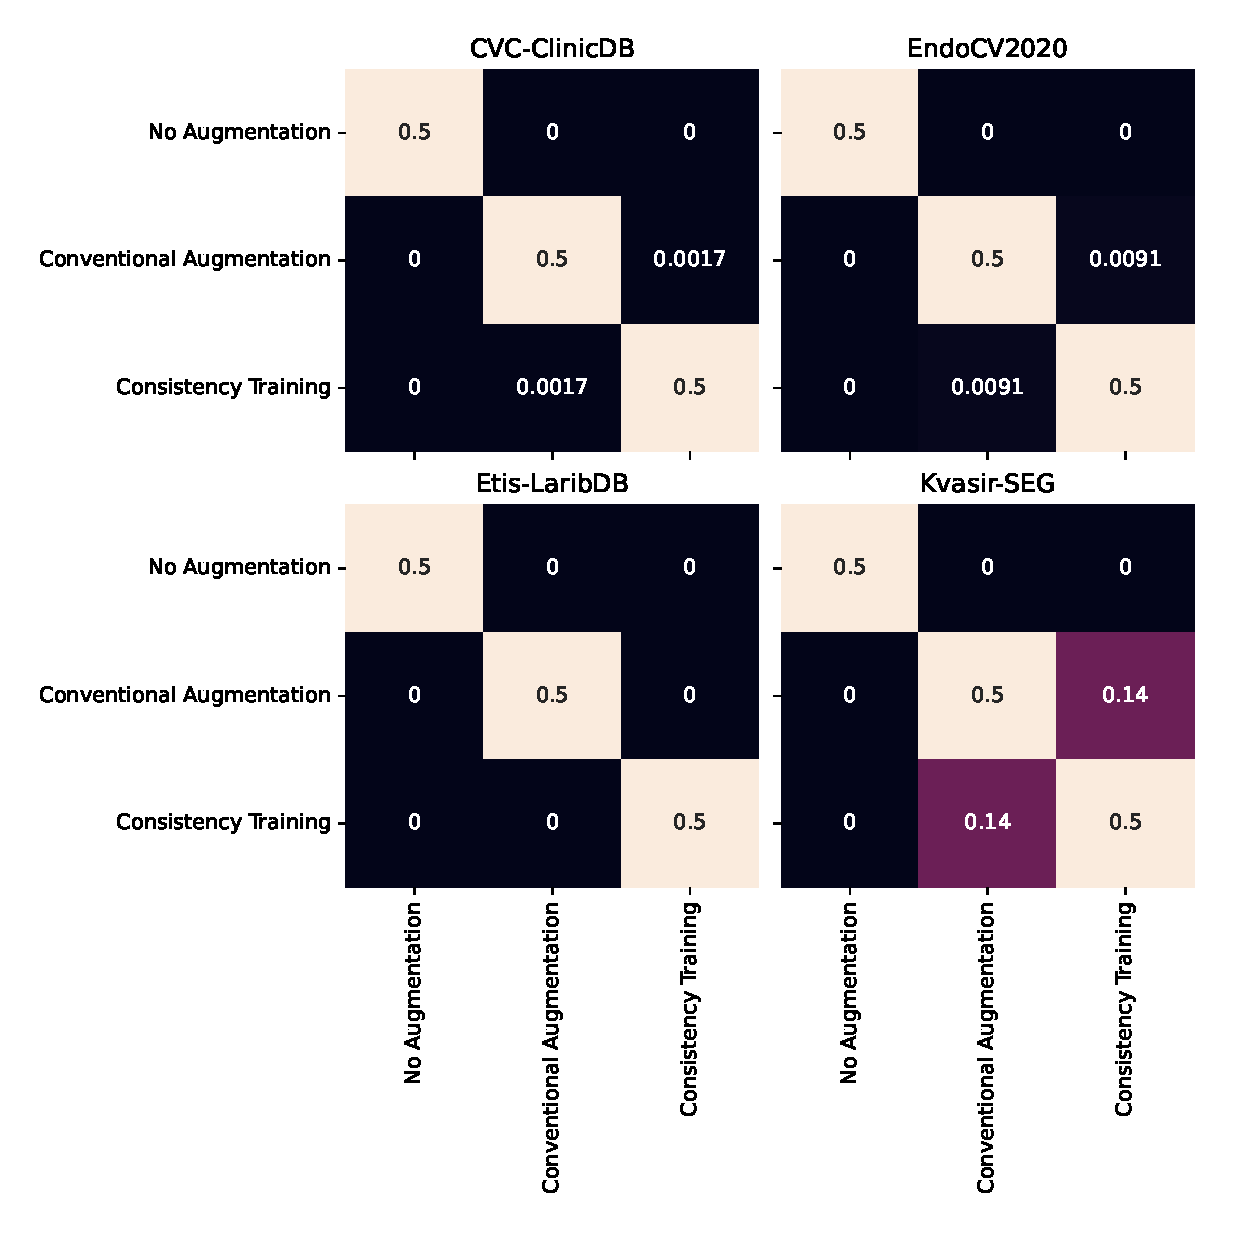
\includegraphics[width=\linewidth]{illustrations/ensemble_relative_pvals.eps}
    \caption[Mann-Whitney U-test results ensembles]{Results from Mann-Whitney U-test for each dataset when comparing the average \glspl{iou} across models for the three training methods. Precision limited to 5 significant figures}
    \label{fig:ttest_training_methods_ensembles}
\end{figure}
    

\newpage
\chapter*{Appendix C: Non-weighted Consistency Training}\label{non_weighted_ctraining}
\addcontentsline{toc}{chapter}{Appendix C: Non-weighted Consistency Training}

\begin{figure}[htb]
    \centering
    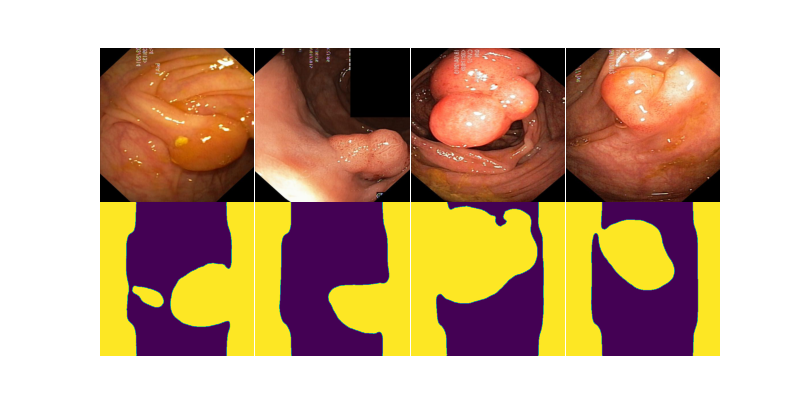
\includegraphics[width=\linewidth]{illustrations/artefacts.png}
    \caption[Unweighted Consistency example]{When the consistency term is not modulated dynamically, the model can quickly learn to predict artifacts around the edges of the image. As polyps can rarely be found in these regions, the consistency term is minimized by predicting consistently wrong predictions where there typically are not polyps. }
    \label{fig:non_weighted_ctraining}
\end{figure}

\chapter*{Appendix D: Paper submitted to NeurIPS2022} \label{Paper}
\addcontentsline{toc}{chapter}{Appendix D: Paper submitted to NeurIPS2022}
\setcounter{chapter}{8}
\setcounter{section}{0}
\setcounter{chapter}{0}
\setcounter{section}{0} 
\includepdf[pages=-]{2022_NIPS_paper_Birk.pdf} 



\end{document}
